\documentclass[a4paper]{scrartcl}

\usepackage{lmodern}
\usepackage[T1]{fontenc}

\usepackage{alltt}
\usepackage[x11names, rgb]{xcolor}
\usepackage{graphicx}
\usepackage{framed}
\usepackage[utf8]{inputenc}
\usepackage{mdwlist}
\usepackage{booktabs}

\usepackage{tikz}
\usetikzlibrary{snakes,arrows,shapes}

\DefineNamedColor{named}{Link}{rgb}{0,0,0.3}
\DefineNamedColor{named}{Cite}{rgb}{0,0.3,0}
\DefineNamedColor{named}{URL}{rgb}{0.3,0,0}

% Platz für Gleitobjekte:
\renewcommand\floatpagefraction{.7}
\renewcommand\topfraction{.8}
\renewcommand\bottomfraction{.5}
\renewcommand\textfraction{.2}



\usepackage[
,colorlinks
,linkcolor=Link
,pagecolor=Link
,citecolor=Cite
,urlcolor=URL
]{hyperref}

\colorlet{cmd}{black!30!red}
\colorlet{rem}{black!60!green}
\colorlet{file}{black!30!blue}
\colorlet{code}{black}
\colorlet{prompt}{black!30}
\colorlet{help}{black!40!red!50!yellow}
\colorlet{bgcolor}{yellow!10}

\newcommand{\textrule}[1]{\par{\noindent\mbox{}\hrulefill #1\hrulefill\par}}
\newcommand{\closerule}{\par\noindent\hrulefill\par}

\newcounter{tcounter}

\newcommand{\tcount}{\makebox[0pt][r]{\tiny\thetcounter~}}

\newenvironment{typed}{\refstepcounter{tcounter}\bgroup\setlength{\topsep}{0pt}\renewcommand{\FrameCommand}[1]{\fcolorbox{black!30}{bgcolor}{##1}\tcount}\MakeFramed{\FrameRestore}\begin{alltt}\small}{\end{alltt}\endMakeFramed\egroup\par\aftergroup\noindent\aftergroup\ignorespaces}
\newenvironment{File}{\bgroup\colorlet{bgcolor}{blue!5}\begin{typed}}{\end{typed}\egroup\aftergroup\ignorespaces}
\newcommand{\file}[1]{\texttt{\color{file}#1}}
\newcommand{\code}[1]{\texttt{\color{code}#1}}
\newcommand{\prompt}{\textcolor{prompt}}
\newcommand{\cmd}[1]{\texttt{\color{cmd}#1}}
\newcommand{\rem}[1]{\texttt{\color{rem}#1}}
\newcommand{\cursor}{\textcolor{black!20!cmd!30}{\raisebox{-.2ex}{\rule{.5em}{2ex}}}}

\newcommand{\rdoc}[1]{\texttt{\color{help}#1}}

\newcommand{\p}{\textcolor{prompt}}
\renewcommand{\c}{\textcolor{cmd}}

\title{WikiExplorator Beginners Tutorial}
\author{Klaus Stein}
\publishers{\vspace{50mm}\par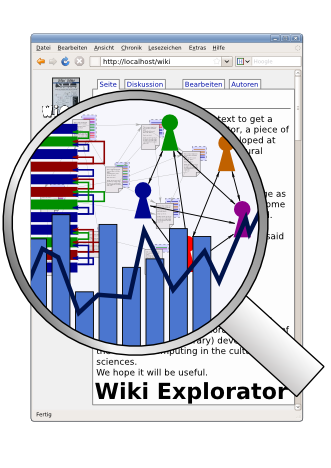
\includegraphics[width=.4\textwidth]{WikiExplorator}\vspace{-1cm}}

\newcounter{fntrdoc}

\begin{document}

\maketitle
\clearpage
\tableofcontents
\clearpage

\section{Introduction}
\label{sec:intro}

WikiExplorator is a ruby toolset and library for wiki exploration. It
allows you to interactively analyse your wiki as well as to generate
nice HTML or PDF reports customized to your needs. This includes
various statistics as well as graph visualizations. The current version
focusses on Mediawiki, other wiki engines can be used with some
tricks.\footnote{If someone wants to contribute a full featured module
for some other wiki engine do not hesitate to contact me, I may be able to
give useful hints.}

In this document I want to give some hints how to use WikiExplorator
in a way that fits your needs. It is a tutorial, not a manual, this
means that all steps given are examples, you will learn one or two
ways to use a certain method or class, but you will not learn about
every possible set of parameters and every method availible. So feel
encuraged to look up the classes and methods used in this tutorial in the
manual\footnote{\url{http://wiki-explorator.rubyforge.org/doc/}}%
\setcounter{fntrdoc}{\thefootnote} and experiment with different
parameter sets.

\section{Installation}
\label{sec:install}

I unpacked the archive to the directory \file{mwparser} and installed
Ruby\footnote{version 1.8.7, version 1.8.6 should also work, if not
  send me a bug report. I testet WikiExplorator on Ruby1.9, but am not
  sure everything works as expected.}, Graphviz, Gnuplot, R, \LaTeX\ and
some Ruby Gems and R packages without problems on (Debian) Linux. For
detailed installation instructions see the \file{INSTALL} file. 

\section{First Steps}
\label{sec:first}

\subsection{Getting Started}
\label{sec:start}

Enter the \file{mwparser} directory and make a copy of
\file{mywikis.rb}. This file will be the personalized startup and
project file, so all customation can be done inside this file. I
recommend to copy this file and save it under another name as
otherwise it would be overwritten when installing new versions.

\begin{typed}
\p{~/mwparser/>} \c{ls} 
html  mediawiki  mediawiki.rb  mywikis.rb  Rakefile.rb  test  util
\p{~/mwparser/>} \c{cp mywikis.rb wio.rb}
\p{~/mwparser/>} \cursor
\end{typed}
I name the new file \file{wio.rb} as our project and its wiki are
named WiO. Now I open \file{wio.rb} with an editor and change it to fit
my environment, looking for the following lines:
\begin{File}
  def Mediawiki.mywiki(pw, options=\{\})
    Wiki.open("wikidb", "localhost", "wikiuser", pw,
              \{:language => 'de', :name => 'MyWiki'\}.merge(options))
  end
\end{File}
Using the class and method documentation\footnotemark[\thefntrdoc] helps
to understand the parameters. The relevant entry is
\rdoc{Mediawiki::Wiki.open}, where some of the parameters are
described and a reference to \rdoc{Mediawiki::DB.new} is given where
the rest of the parameters is documented. To fit everything to my
environment I change the name of the database to \file{wiodb}, give
the database host, the database user and the name and language of the
wiki\footnote{if our tables have some prefix ``\code{xxx}'', we would
  add \cmd{:prefix => 'xxx'} within the braces.}:\footnote{if you have
to use ODBC to access your database the second example should fit your
needs}
\begin{File}
  def Mediawiki.mywiki(pw, options=\{\})
    Wiki.open("wiodb", "wiowiki.kinf.wiai.uni-bamberg.de", "wiouser", pw,
              \{:language => 'de', :name => 'WiO'\}.merge(options))
  end
\end{File}
All of this information can be found by looking into
\file{LocalSettings.php}\footnote{note that \file{localhost} must be
  replaced by the actual hostname if you want to remotely access the
  database. In this case additionally Mysql must allow remote access
  (globally and for this user).}.

So, let's see if everything works:\footnote{the password can also
be found in \file{Localsettings.php}}
\begin{typed}
\p{~/mwparser/>} \c{ruby wio.rb}
Tools for Social Network Analysis
[\dots]

Connecting to your wiki ...
Password: \c{\textit{secret}}

Connecting to your wiki ...
Password: 
connecting to database wiowiki.kinf.wiai.uni-bamberg.de/wiodb
connected.
Table wio_genres in DB not found
Table wio_roles in DB not found
users: 15
revisions: 1362
timeline length: 1352
firsttime: Di Mär 20 18:23:15 UTC 2007
lasttime: Di Jul 28 13:53:09 UTC 2009
Done.
Avg. # of users: 1.8348623853211
# of pages with more than one user: 57/109 (52.29%)

give "report" as command line parameter to create a pdf report of your wiki.

\p{~/mwparser/>} \cursor
\end{typed}
This looks fine. Our wiki has 15 users and 1352 edits, had the first
edit in March 2007 and the last one in July 2009.

\clearpage

\subsection{Interactive Usage}
\label{sec:interactive}

So let's see what WikiExplorator can tell about our wiki. We use the
interactive ruby shell \file{irb}:\footnote{instead of \cmd{wio} you
  certainly use whatever you called your project file}
\begin{typed}
\p{~/mwparser/>} \c{irb -r wio}
Tools for Social Network Analysis
\dots
\p{irb(main):001:0>} \cursor
\end{typed}
The parameter ``\code{-r wio}'' means: require the library \code{wio}
which is our project file.

The next step is to open our wiki:
\begin{typed}
\p{irb(main):001:0>} \c{wiki = Mediawiki.mywiki('\textit{secret}')}
connecting to database wiowiki.kinf.wiai.uni-bamberg.de/wiodb
connected.
Table wio_genres in DB not found
Table wio_roles in DB not found
users: 15
revisions: 1362
timeline length: 1352
firsttime: Di Mär 20 18:23:15 UTC 2007
lasttime: Di Jul 28 13:53:09 UTC 2009
Done.
=> #<Mediawiki::Wiki WiO: wiowiki.kinf.wiai.uni-bamberg.de/wiodb, 
271 pages, 1362 revisions, 15 users>
\p{irb(main):002:0>} \cursor
\end{typed}
Now the variable \code{wiki} holds the wiki object (see
\rdoc{Mediawiki::Wiki} in the manual) and we can start to investigate:
\begin{typed}
\p{irb(main):002:0>} \c{wiki.users.length}
=> 15
\p{irb(main):003:0>} \c{wiki.pages.length}
=> 109
\p{irb(main):004:0>} \c{wiki.revisions.length}
=> 1125
\end{typed}
We ask the wiki to give us the users and count their length, we have
15 users, fine. Same for the pages, we have 109 pages. And finally for
the revisions: 1125. But wait! Shouldn't this be 1352? There is
something wrong.

This is caused by the fact that by default only namespace 0 (the main
wiki namespace) is taken into account, so we habe 109 pages and 1125
revisions in namespace 0. We will learn soon how to change this by
using filters (section~\ref{sec:filters}).

\bigskip

For the moment we will see what the wiki can tell us using some
ruby. I cannot provide a full-featured Ruby introduction within this
tutorial but I will try to give some hints.\footnote{use
  \url{http://www.ruby-lang.org/} as a starting point for information
  about Ruby. You may at least need some Ruby knowledge when things
start to get more sophisticated.}

We may also be interested in a single user. Let's fetch the first one
from our wiki's user collection:
\cmd{wiki.users} gives a collection of User objects (see
\rdoc{Mediawiki::User}), and the method \cmd{first} gives the first
entry in this collection:
\begin{typed}
\p{irb(main):005:0>} \c{user = wiki.users.first}
=> #<Mediawiki::User id=5 name="Regina">
\end{typed}
In Ruby every method has a return value and irb indicates the returned
object with ``\code{=>}''. Normally a condensed string representation
of the object is given. 

We could also have asked the wiki for user Regina:
\begin{typed}
\p{irb(main):217:0>} \c{user = wiki.user_by_name('Regina')}
=> #<Mediawiki::User id=5 name="Regina">
\end{typed}
This certainly gives us the same object.

Now we can ask this user a lot of neat things:
\begin{typed}
\p{irb(main):006:0>} \c{user.uid}
=> 5
\p{irb(main):007:0>} \c{user.name}
=> "Regina"
\p{irb(main):008:0>} \c{user.real_name}
=> "Regina Meister"
\p{irb(main):009:0>} \c{user.revisions.length}
=> 105
\p{irb(main):010:0>} \c{user.pages.length}
=> 18
\end{typed}
So Regina has 105 edits on 18 pages. Wouldn't it be nice to have a
list of all users with their pages and edits? We only need to ask each
user for his pages and his revisions, count them and collect this
information:
\begin{typed}
\p{irb(main):011:0>} \c{wiki.users.collect \{ |u|
                     [u.name, u.pages.length, u.revisions.length] \}}
=> [["Regina", 18, 105], ["Sissi", 0, 0], ["system", 1, 1], ["August", 1, 1], 
    ["Tom", 17, 63], ["WikiSysop", 0, 0], ["Fritz", 20, 87], ["Olga", 21, 103],
    ["Klaus", 45, 151], ["Carla", 0, 0], ["Sam", 2, 9], ["Caro", 0, 0], 
    ["Dan", 2, 6], ["Steffen", 71, 594], ["Helga", 2, 5]]
\end{typed}

Some words about the syntax: we ask the wiki object about its users
(call the method \cmd{users} on it), this returns a collection of
users on which we now call the method \cmd{collect} which takes a
block as a parameter. A block is a piece of code given in
braces\footnote{you can also use \cmd{do} \dots\,\cmd{end} instead of
  \cmd{\{} \dots\,\cmd{\}}} taking one or more parameters given in
pipes (\cmd{|u|}). \cmd{collect} calls the block given for every member of
the collection and returns the results of the block in a large array.
\bigskip

Fortunately there is an auxiliary method which pretty prints (pp)
these statistics (the columns are explained in the manual: 
\rdoc{Mediawiki::Wiki.pp\_userstats}):
\begin{typed}
\p{irb(main):013:0>} \c{wiki.pp_userstats}
user         realname                 uid    e    p    e/p   se   fe   ke   ie
===============================================================================
August       August Kaiser              6    1    1   1.00    0    1    0    0
Carla        Carla Schach               8    0    0    nan    0    0    0    0
Caro         Carol Heart                9    0    0    nan    0    0    0    0
Dan          Dan Bosco                 15    6    2   3.00    2    4    0    1
Fritz        Fritz Lost                 7   87   20   4.35   55   27    0    1
Helga        Helga Mayer               10    5    2   2.50    3    1    0    0
Klaus        Klaus Stein                2  151   45   3.36   81   42    0    7
Olga         Olga Kranz                13  103   21   4.90   72   18    0    0
Regina       Regina Meister             5  105   18   5.83   73   31    0    0
Sam          Sam Hawkins               14    9    2   4.50    6    3    0    2
Sissi        Sissi Helfer              11    0    0    nan    0    0    0    0
Steffen      Steffen Blaschke           4  594   71   8.37  458   83    0   27
Tom          Tom Toppler               12   63   17   3.71   43   13    0    0
WikiSysop                               1    0    0    nan    0    0    0    0
system       System User                0    1    1   1.00    0    0    0    0
=> nil
\end{typed}
Hm, and the other way around? How many users on each page?
\begin{typed}
\p{irb(main):031:0>} \c{wiki.pages.collect \{ |p| p.users.length \}}
=> [1, 1, 1, 3, 1, 1, 7, 2, 1, 1, 1, 1, 3, 1, 1, 2, 1, 2, 1, 1, 1, 3, 2, 4, 2, 
    5, 1, 2, 3, 1, 4, 1, 2, 3, 1, 2, 1, 2, 2, 2, 1, 3, 2, 1, 1, 2, 2, 4, 2, 2, 
    2, 4, 1, 5, 1, 2, 2, 1, 1, 1, 2, 2, 1, 1, 1, 2, 1, 3, 2, 2, 1, 2, 1, 2, 1, 
    2, 1, 2, 1, 3, 1, 2, 1, 2, 2, 4, 2, 3, 1, 2, 2, 2, 1, 1, 2, 2, 1, 4, 1, 1, 
    1, 1, 4, 1, 1, 1, 1, 1, 2]
\end{typed}
Not very clear. Perhaps a histogram with the number of pages for each user? 
\begin{typed}
\p{irb(main):037:0>} \c{wiki.pages.collect \{ |p| p.users.length \}.stat_histogram}
=> \{5=>2, 1=>52, 7=>1, 2=>38, 3=>9, 4=>7\}
\end{typed}
That's better, but not good. We try some pseudographics:
\begin{typed}\label{typed:pu}
\p{irb(main):047:0>} \c{pu = wiki.pages.collect \{ |p| p.users.length \}.stat_histogram}
=> \{5=>2, 1=>52, 7=>1, 2=>38, 3=>9, 4=>7\}
\p{irb(main):048:0>} \c{pu.keys.min.upto(pu.keys.max) \{ |k|
                     puts(('%2i: ' % k) + ('#' * pu[k])) \}}
 1: ####################################################
 2: ######################################
 3: #########
 4: #######
 5: ##
 6: 
 7: #
=> 1
\end{typed}
The \cmd{'\%2i:\ '} is a printf expression as known from C.

\clearpage

\begin{figure}
  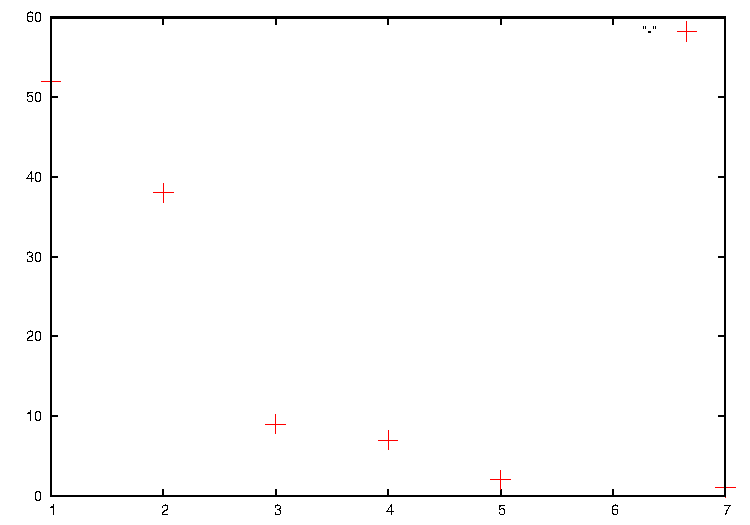
\includegraphics[width=.49\textwidth]{gp_hist_points}\hfill
  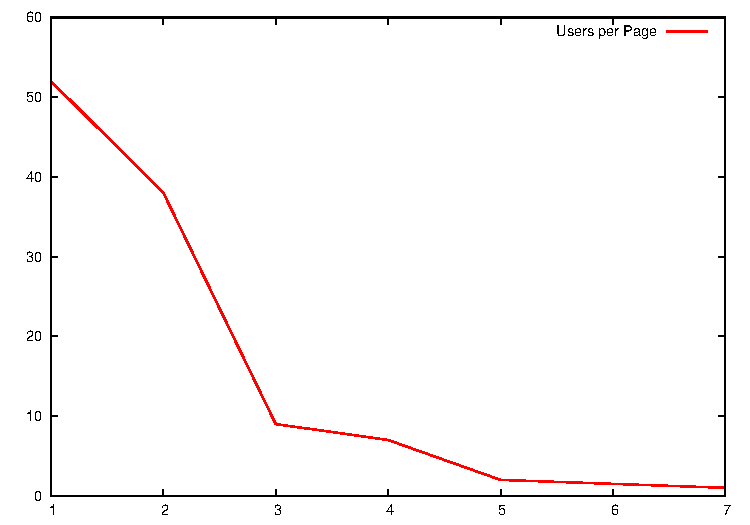
\includegraphics[width=.49\textwidth]{gp_hist_line}\\
  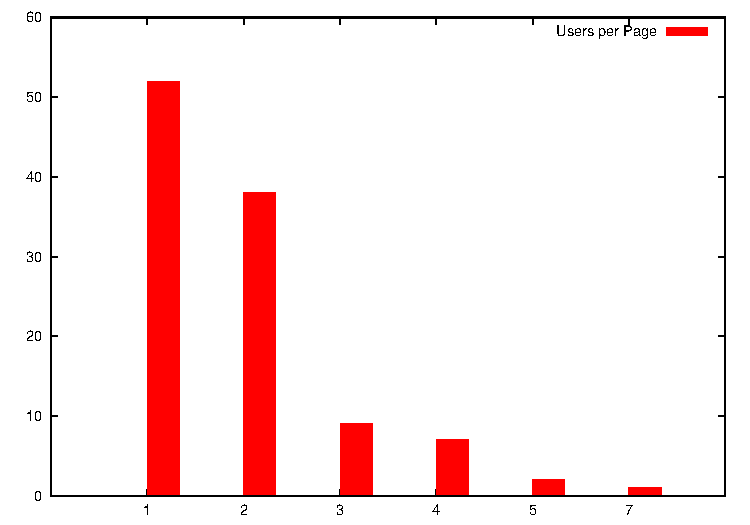
\includegraphics[width=.49\textwidth]{gp_hist_hist0}\hfill
  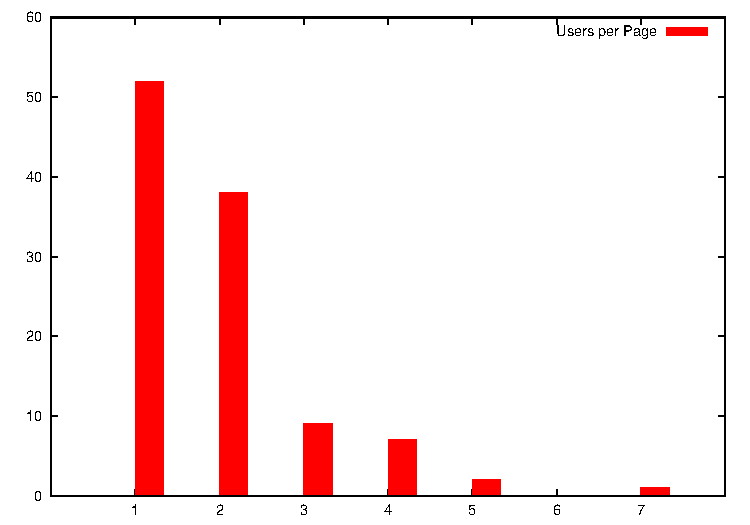
\includegraphics[width=.49\textwidth]{gp_hist_hist}
  \caption{Using Gnuplot for data presentation}
  \label{fig:gp_hist}
\end{figure}

\section{Gnuplot}
\label{sec:gnuplot}

Let's use gnuplot for a graphical representation of this
histogram:\footnote{using \cmd{pu} as defined in session~\ref{typed:pu}}
\begin{typed}
\p{irb(main):051:0>} \c{pu.gp_plot}
=> #<Gnuplot:0xf6733cf4 ... >
\p{irb(main):061:0>} \c{pu.sort.gp_plot(:title => 'Users per Page', :with => 'lines')}
=> #<Gnuplot:0xf66f32a8 ...>
\p{irb(main):070:0>} \c{pu.sort.gp_plot(:title => 'Users per Page',
                     :using => '2:xtic(1)', :with => 'histograms fill solid')}
=> #<Gnuplot:0xf66b60c4 ...>
\end{typed}
First we simply plotted the data using gnuplot
(figure~\ref{fig:gp_hist} top left), then the same using a line and
adding a title (top right). Note that we had to sort the data
before. Try out what happens otherwise. And finally we tried the
histogram (bottom left). It looks fine but has one problem: it would
be nice if we get an empty column with label 6 between 5 and 7. Let's
see how to do this (figure~\ref{fig:gp_hist} bottom right):
\begin{typed}
\p{irb(main):072:0>} \c{(pu.keys.min..pu.keys.max).collect \{ |k| [k, pu[k]]
                      \}.gp_plot(:title => 'Users per Page',
                      :using => '2:xtic(1)', :with => 'histograms fill solid')}
=> #<Gnuplot:0xf66807d0 ...>
\end{typed}
\begin{figure}
  \parbox[b]{.5\textwidth}{%
  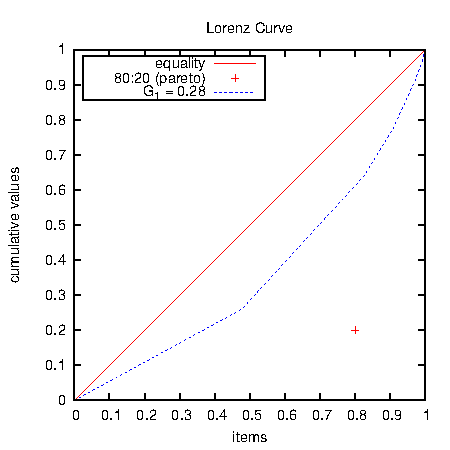
\includegraphics[width=\linewidth]{gp_lorenz}
  \caption{Lorenz curve for users per page}
  \label{fig:gp_lorenz}}\hfill
  \parbox[b]{.485\textwidth}{%
  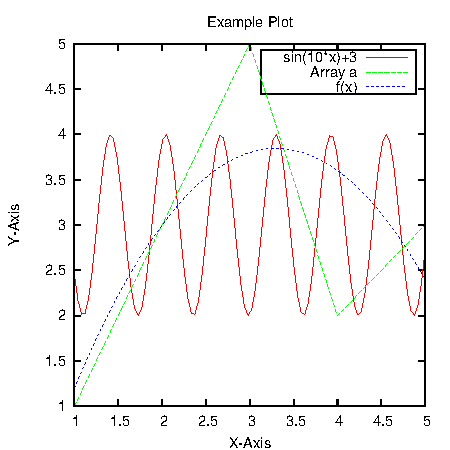
\includegraphics[width=\linewidth]{gp_example}\vspace{1mm}
  \caption{Extended gnuplot example}
  \label{fig:gp_example}}
\end{figure}
On the other hand, the data (users per page) is as if predestined to
be presented as a Lorenz
curve\footnote{\url{http://en.wikipedia.org/wiki/Lorenz_curve}}, so
let's see what we get (figure~\ref{fig:gp_lorenz}):
\begin{typed}
\p{irb(main):107:0>} \c{wiki.pages.collect \{ |p| p.users.length \}.gp_plot_lorenz}
=> #<Gnuplot:0xf64c3258 ...
 ... lines and lines of output ...
 ... >
\end{typed}
Nice picture. But irb disturbed me with printing so many lines of
output for the gnuplot object. We can fix this by adding another
command with less output (we just use nil):
\begin{typed}
\p{irb(main):107:0>} \c{wiki.pages.collect \{ |p| p.users.length \}.gp_plot_lorenz; nil}
=> nil
\end{typed}
Fine. But gnuplot is more. See
\url{http://gnuplot.sourceforge.net/demo_4.2/} for examples about what
gnuplot can do. And certainly all of this is accessible from
WikiExplorator, including function fitting etc. (see also the examples
in \rdoc{Gnuplot.new}, \rdoc{Gnuplot.fit}). I give you a small example
for extended gnuplot usage at figure~\ref{fig:gp_example} using an
array \cmd{a} and the function \cmd{$\sin(10x)+3$}:
\begin{typed}
\p{irb(main):111:0>} \c{a = [[1,1], [2,3], [3,5], [4,2], [5,3]]}
=> [[1, 1], [2, 3], [3, 5], [4, 2], [5, 3]]
\p{irb(main):127:0>} \c{Gnuplot.new do |gp|}
\p{irb(main):128:1*} \c{  gp.add('sin(10*x)+3')}
\p{irb(main):129:1>} \c{  gp.add(a, :with => 'lines', :title => 'Array a')}
\p{irb(main):130:1>} \c{  gp.fit(:function => 'f(x) = a*x**2 + b*x + c', :via => 'a,b,c')}
\p{irb(main):131:1>} \c{  gp.title = 'Example Plot'}
\p{irb(main):132:1>} \c{  gp.set('key','box')}
\p{irb(main):133:1>} \c{  gp.set('xlabel', 'X-Axis', true)}
\p{irb(main):134:1>} \c{  gp.set('ylabel', 'Y-Axis', true)}
\p{irb(main):135:1>} \c{  gp.plot}
\p{irb(main):136:1>} \c{end}
...
=> #<Gnuplot:0xf7a5e3c4 ... >
\end{typed}
So one thing is left: we want the graphics to be saved, either as
bitmap or as vector graphics. So let's plot our example array \cmd{a}
to file\footnote{\label{fnt:pspdf}you may need to use \cmd{:pspdf} instead of
  \cmd{:pdf} if your gnuplot has no native PDF support}:
\begin{typed}
\p{irb(main):184:0>} \c{a.gp_plot(:with => 'lines', :png => 'example.png')}
=> #<Gnuplot:0xf6753400 ...>
\p{irb(main):185:0>} \c{a.gp_plot(:with => 'lines', :svg => 'example.svg')}
=> #<Gnuplot:0xf674c920 ...>
\p{irb(main):186:0>} \c{a.gp_plot(:with => 'lines', :pdf => 'example.pdf')}
=> #<Gnuplot:0xf6745c74 ...>
\end{typed}

\clearpage

\begin{figure}
  \parbox[b]{.5\textwidth}{%
    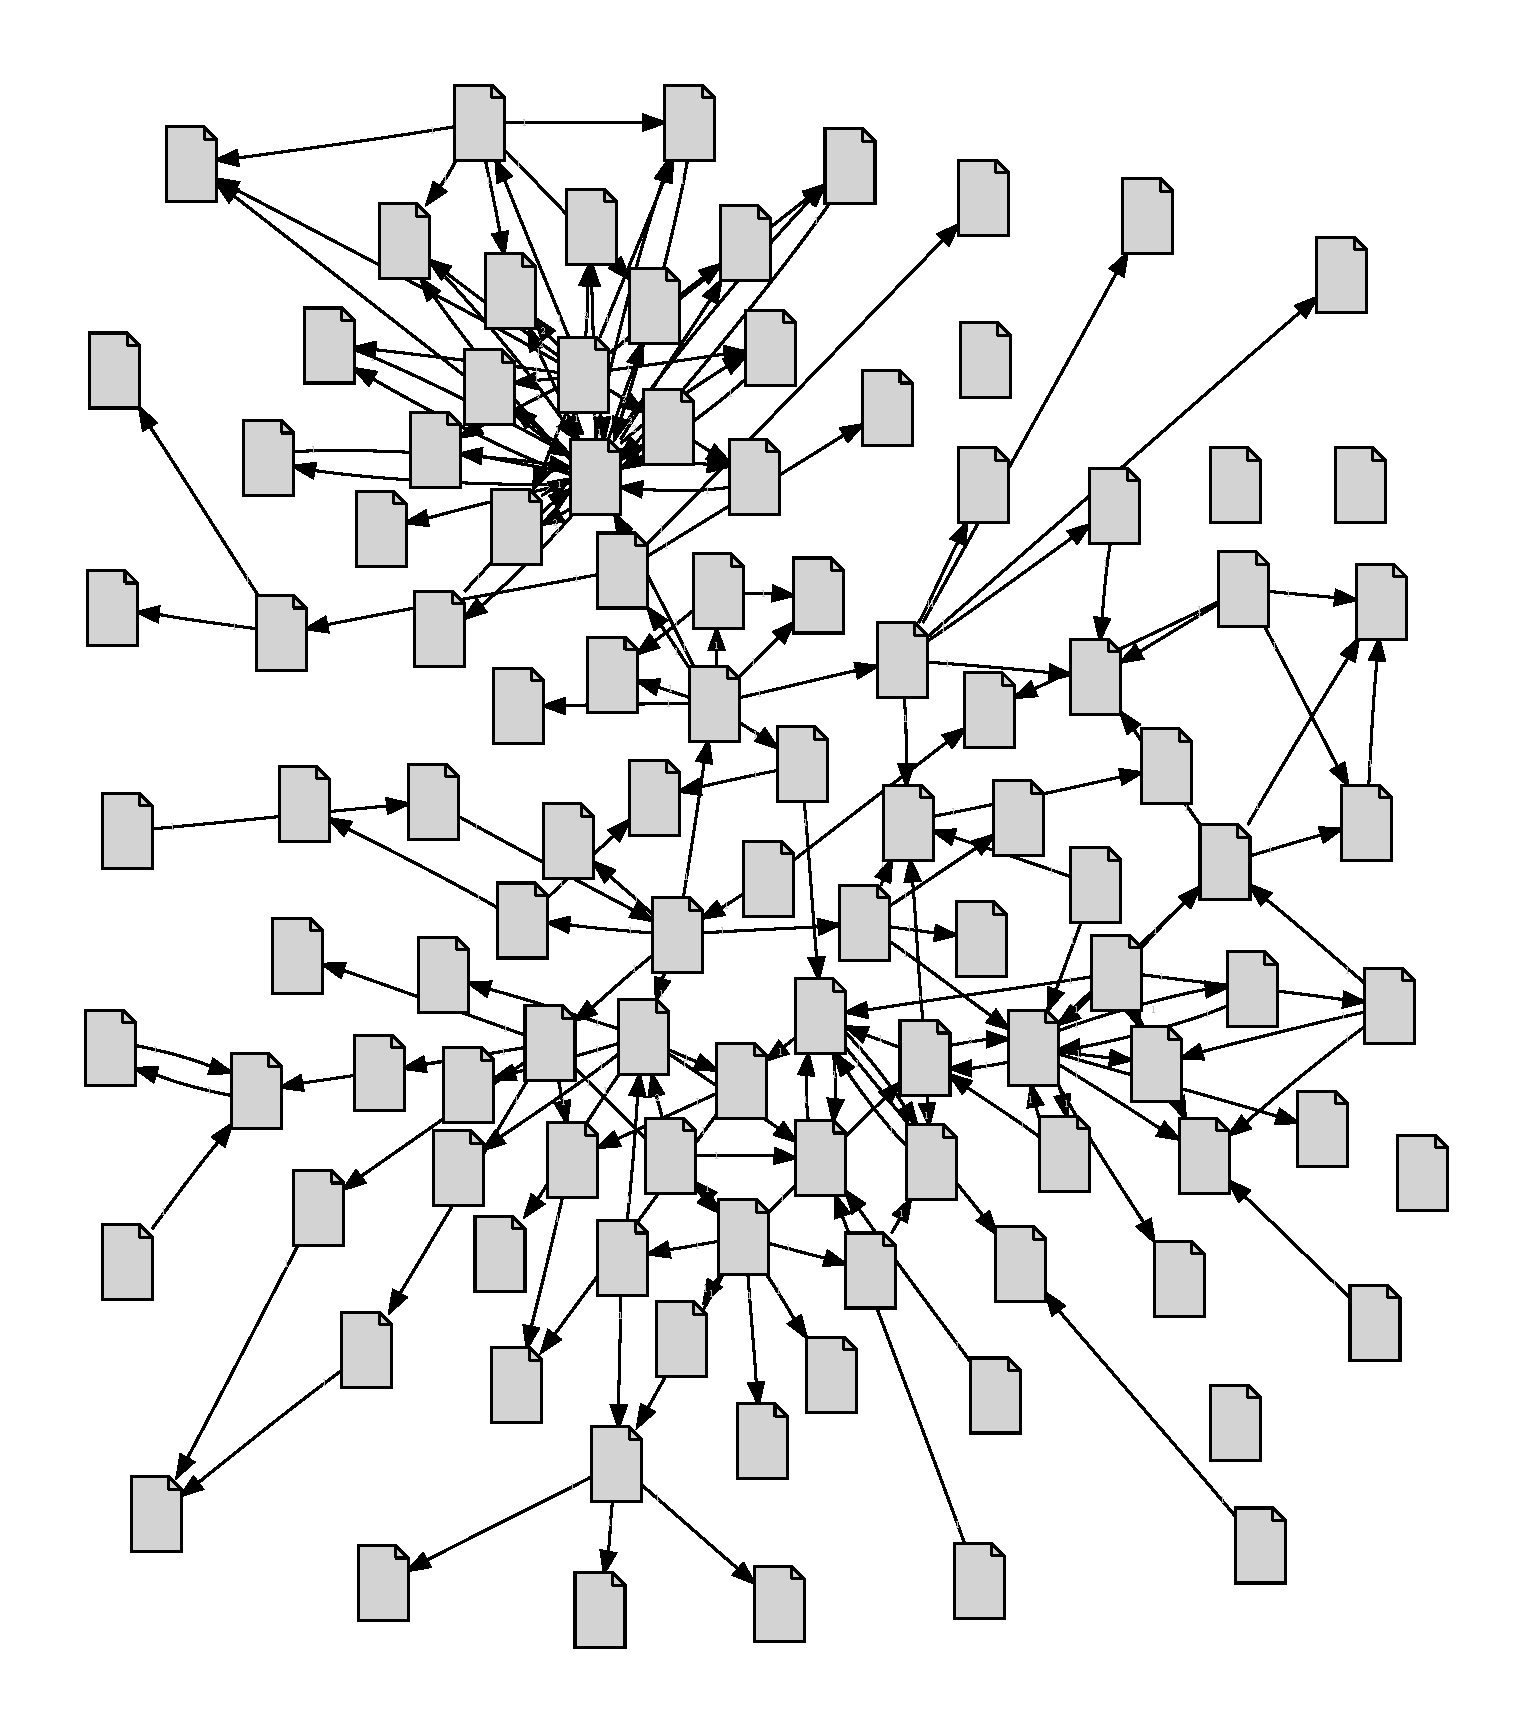
\includegraphics[width=\linewidth]{gv_pagegraph}
    \caption{hyperlink network}
    \label{fig:hyperlink}
  }%
  \parbox[b]{.5\textwidth}{%
    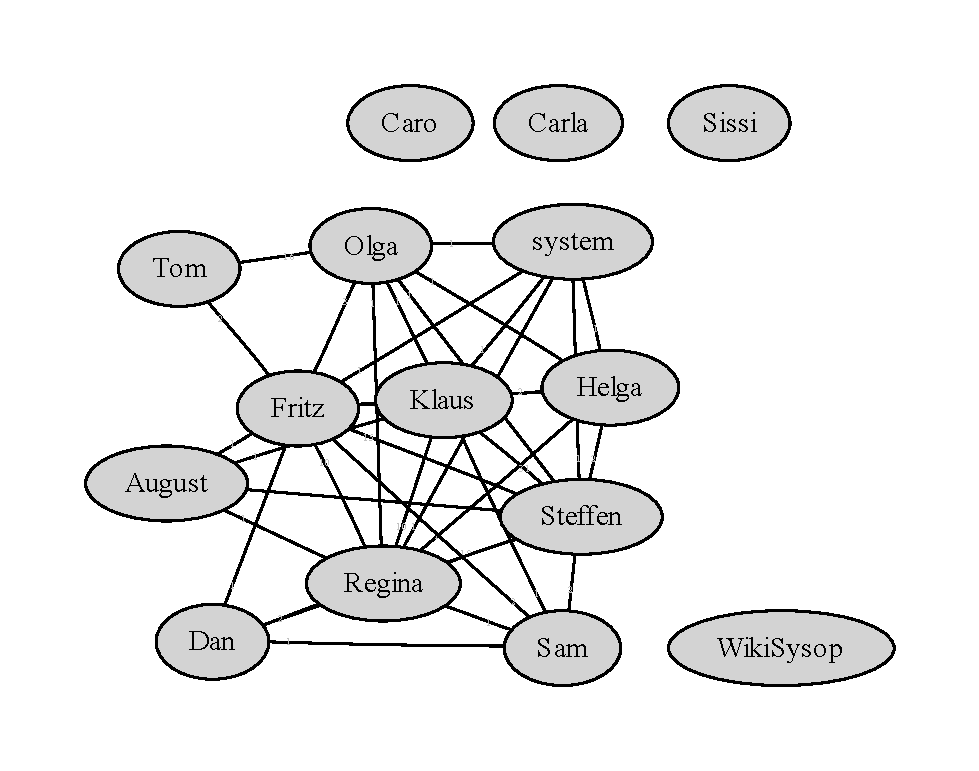
\includegraphics[width=\linewidth]{gv_coauthorgraph-full}\vspace{1cm}
    \caption{coauthorship network}
    \label{fig:coauthor}
  }
\end{figure}

\section{Network Graphs}
\label{sec:network}

Many aspects of a wiki can be represented as networks. The most
obvious networks are the page hyperlink graph
(figure~\ref{fig:hyperlink}) where the nodes represent the wiki pages
and the (directed) edges give the links between the pages, and the
coauthorship network (figure~\ref{fig:coauthor}) where the nodes
represent the wiki authors and two authors are connected with a link
if they edited the same page.\footnote{more precisely: two authors are
  connected by an edge if there exists at least one page both did at
  least edit once.}

As we will see soon a lot of varieties of these as well as different
graphs are available.

\subsection{First Steps}
\label{sec:dotgraphintro}

We start with asking the wiki for the coauthorshipgraph:
\begin{typed}
\p{irb(main):030:0>} \c{cgraph = wiki.coauthorgraph}
=> #<DotGraph:0xf779a2c8 ...>
\end{typed}
This gives us a \cmd{DotGraph} object representing the network. 
This DotGraph object can now be used to compute various network
measures and to visualize the graph in different ways.
Most of the methods work on directed and undirected graphs, some also
respect edge weights.

We start with
some statistics about the degree distribution, sorted by user name
(\rdoc{DotGraph.pp\_degrees}):
\begin{typed}
\p{irb(main):049:0>} \c{cgraph.pp_degrees(:sortby => :node, :up => true)}
Node                          :  deg
August                        :    4
Carla                         :    0
Caro                          :    0
Dan                           :    4
Fritz                         :   10
Helga                         :    6
Klaus                         :    8
Olga                          :    7
Regina                        :    9
Sam                           :    5
Sissi                         :    0
Steffen                       :    9
Tom                           :    2
WikiSysop                     :    0
system                        :    6
=> nil
\end{typed}
So Fritz is connected to most of the others, directly followed by
Regina and Steffen. On a second thought, we are not interested on
nodes not connected to others, so we remove them, and then we print
our list again, now with user real names and sorted by degree:
\begin{typed}\label{typed:remove_lonely_nodes}
\p{irb(main):065:0>} \c{cgraph.remove_lonely_nodes; nil}\footnotemark
=> nil
\p{irb(main):066:0>} \c{cgraph.pp_degrees(:sortby => :degree) \{ |u| u.real_name \}}
Node                          :  deg
Fritz Lost                    :   10
Steffen Blaschke              :    9
Regina Meister                :    9
Klaus Stein                   :    8
Olga Kranz                    :    7
Helga Mayer                   :    6
System User                   :    6
Sam Hawkins                   :    5
August Kaiser                 :    4
Dan Bosco                     :    4
Tom Toppler                   :    2
=> nil
\end{typed}
That's better. Now the ranking is obvious.%
\footnotetext{You remember: the \cmd{nil} is only given to suppress
  the (rather lengthy) return output}
We used the \code{pp\_degrees} method in the example to get pretty
output (\code{pp} stands for ``pretty print''). For further processing
we could have used \code{degrees} which gives the raw data. Some but
not all methods have \code{pp\_} counterparts for convenience. So when
I use a \code{pp\_} method in the following examples have a look at
the pure method.

\subsection{R}
\label{sec:Rintro}

If \file{R} and \file{rsruby} are installed and working (and the
required \file{R} libraries are installed) we can access all of the
network measures \file{R} (or rather the \file{R} library \file{sna})
provides using ruby. The method documentation states which
\code{DotGraph} methods are based on \file{R}. So we can
e.\,g. compute betweenness, closeness and others (for full
\file{R} access see \rdoc{util/r.rb} in the manual):
\begin{typed}
\p{irb(main):093:0>} \c{cgraph.pp_betweenness(:sortby => :value)}
Node                          :          betweenness
============================================================
Fritz                         :         8.8333333333
Steffen                       :         3.3333333333
Regina                        :         3.3333333333
Olga                          :         2.5000000000
Klaus                         :         1.7500000000
Sam                           :         0.2500000000
Helga                         :         0.0000000000
Dan                           :         0.0000000000
August                        :         0.0000000000
Tom                           :         0.0000000000
system                        :         0.0000000000
=> nil
\p{irb(main):094:0>} \c{cgraph.pp_closeness(:sortby => :value)}
Node                          :            closeness
============================================================
Fritz                         :         1.0000000000
Steffen                       :         0.9090909091
Regina                        :         0.9090909091
Klaus                         :         0.8333333333
Olga                          :         0.7692307692
Helga                         :         0.7142857143
system                        :         0.7142857143
Sam                           :         0.6666666667
August                        :         0.6250000000
Dan                           :         0.6250000000
Tom                           :         0.5555555556
=> nil
\end{typed}

\subsection{Graph Visualization}
\label{sec:gvis}

\begin{figure}
\parbox[b]{0.7\textwidth}{
  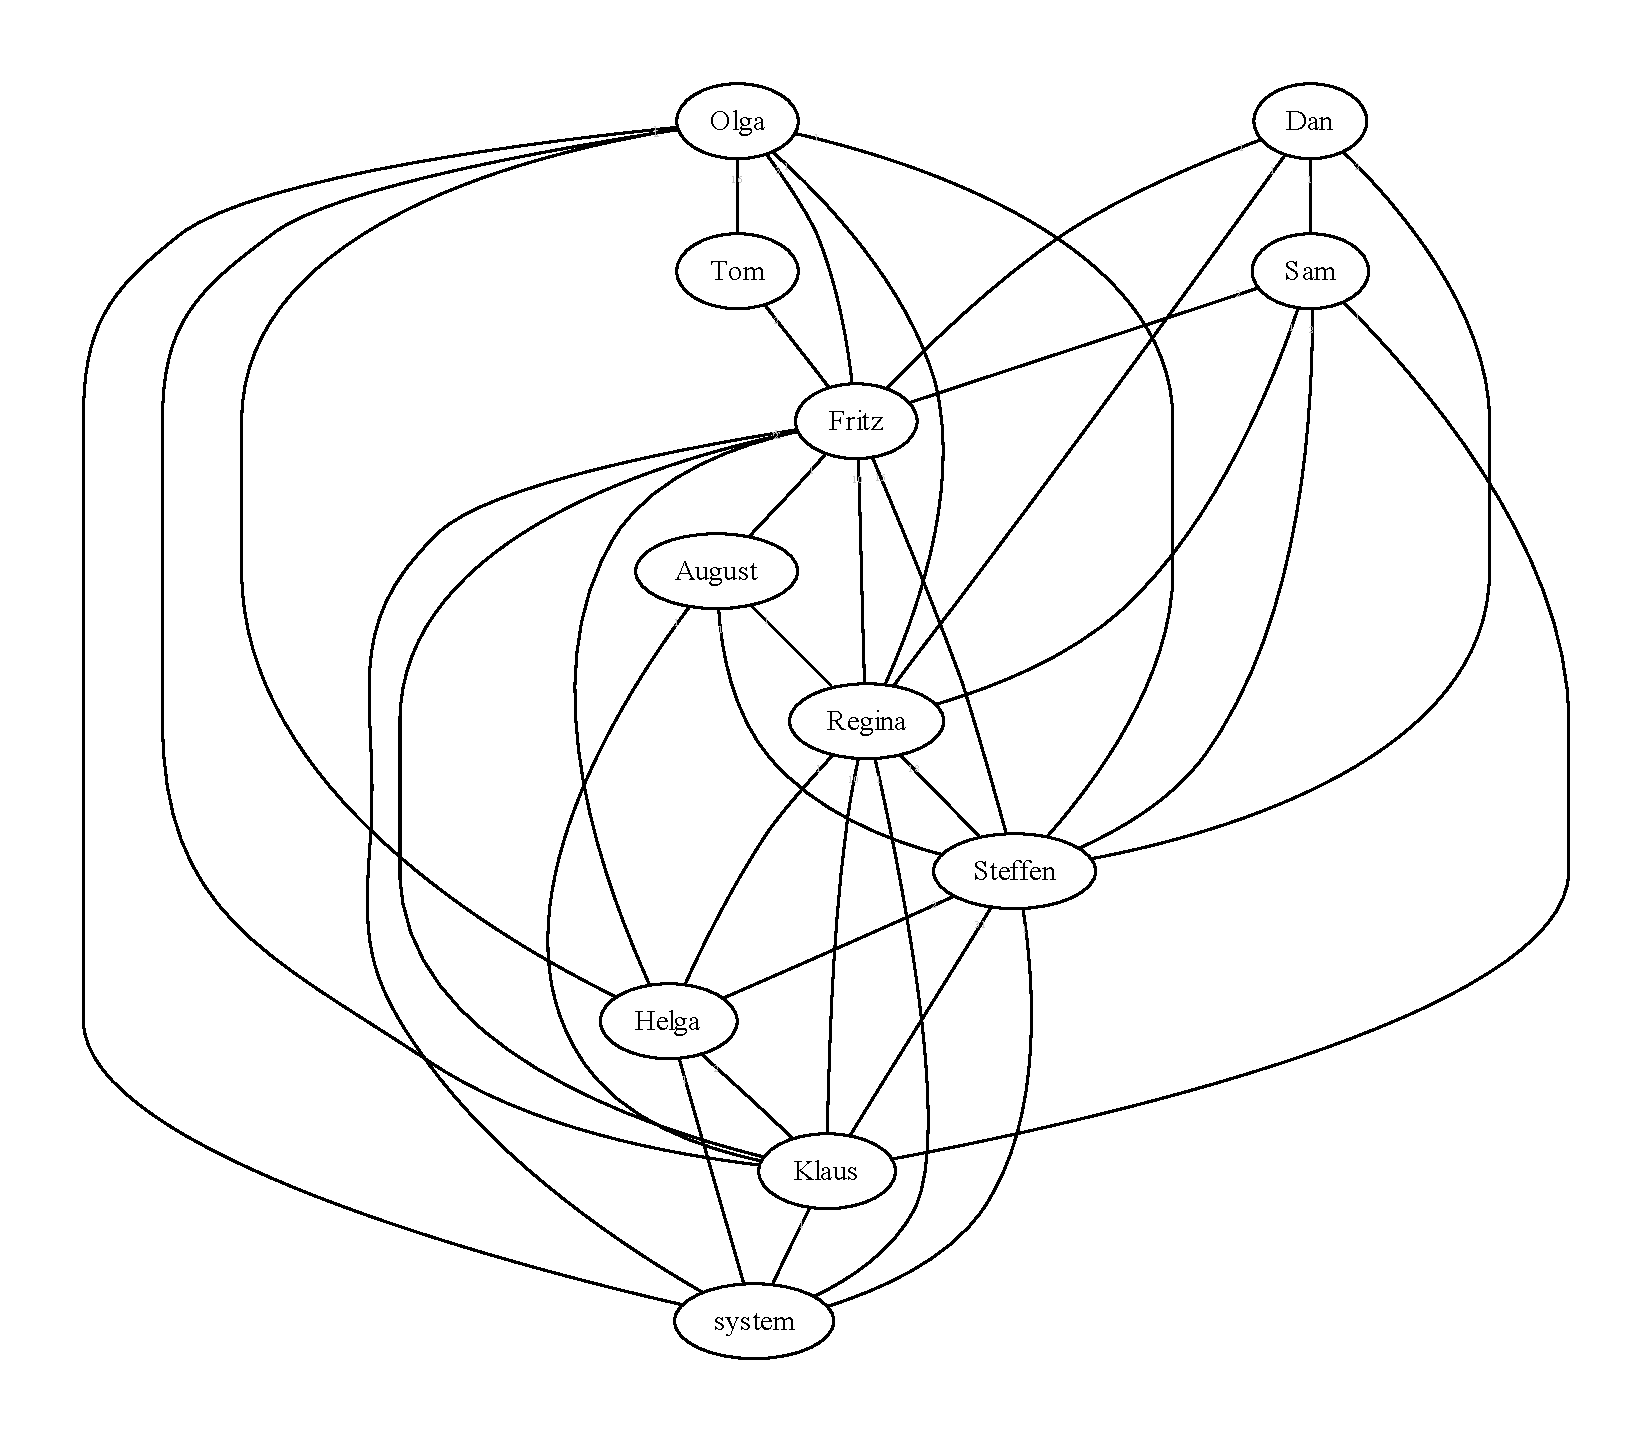
\includegraphics[width=\linewidth]{gv_ca-dot}\vspace{-7mm}
  \caption{\code{dot} layout}
  \label{fig:gv-cadot}}%
\parbox[b]{0.3\textwidth}{\centering
  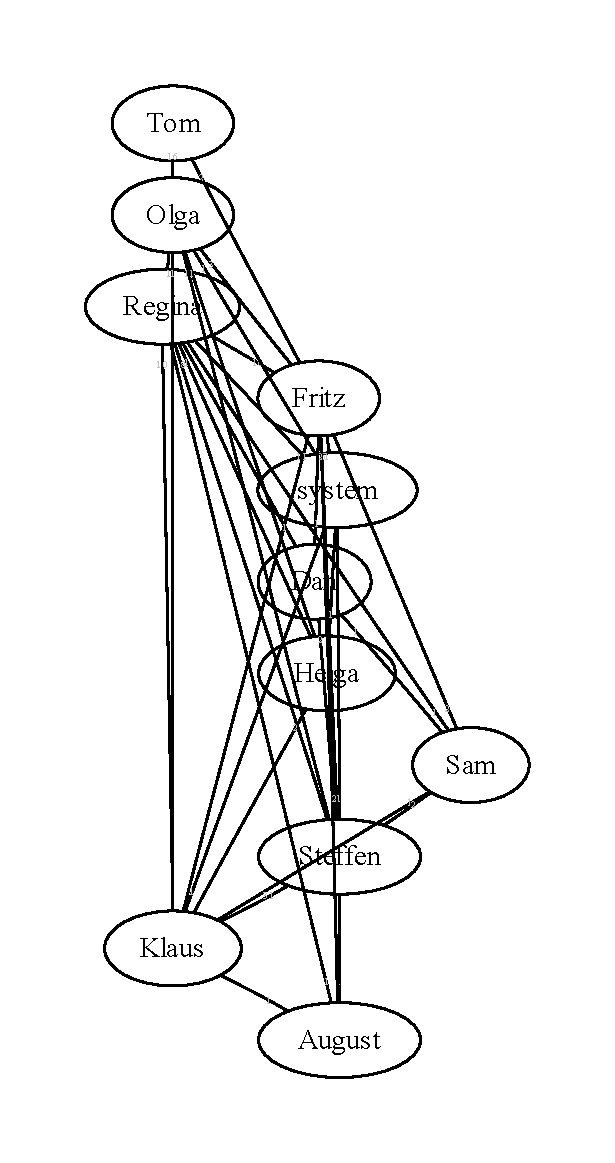
\includegraphics[width=\linewidth]{gv_ca-fdp}
  \caption{\code{fdp} layout}
  \label{fig:gv-cafdp}}\\
\parbox[b]{0.7\textwidth}{\centering
  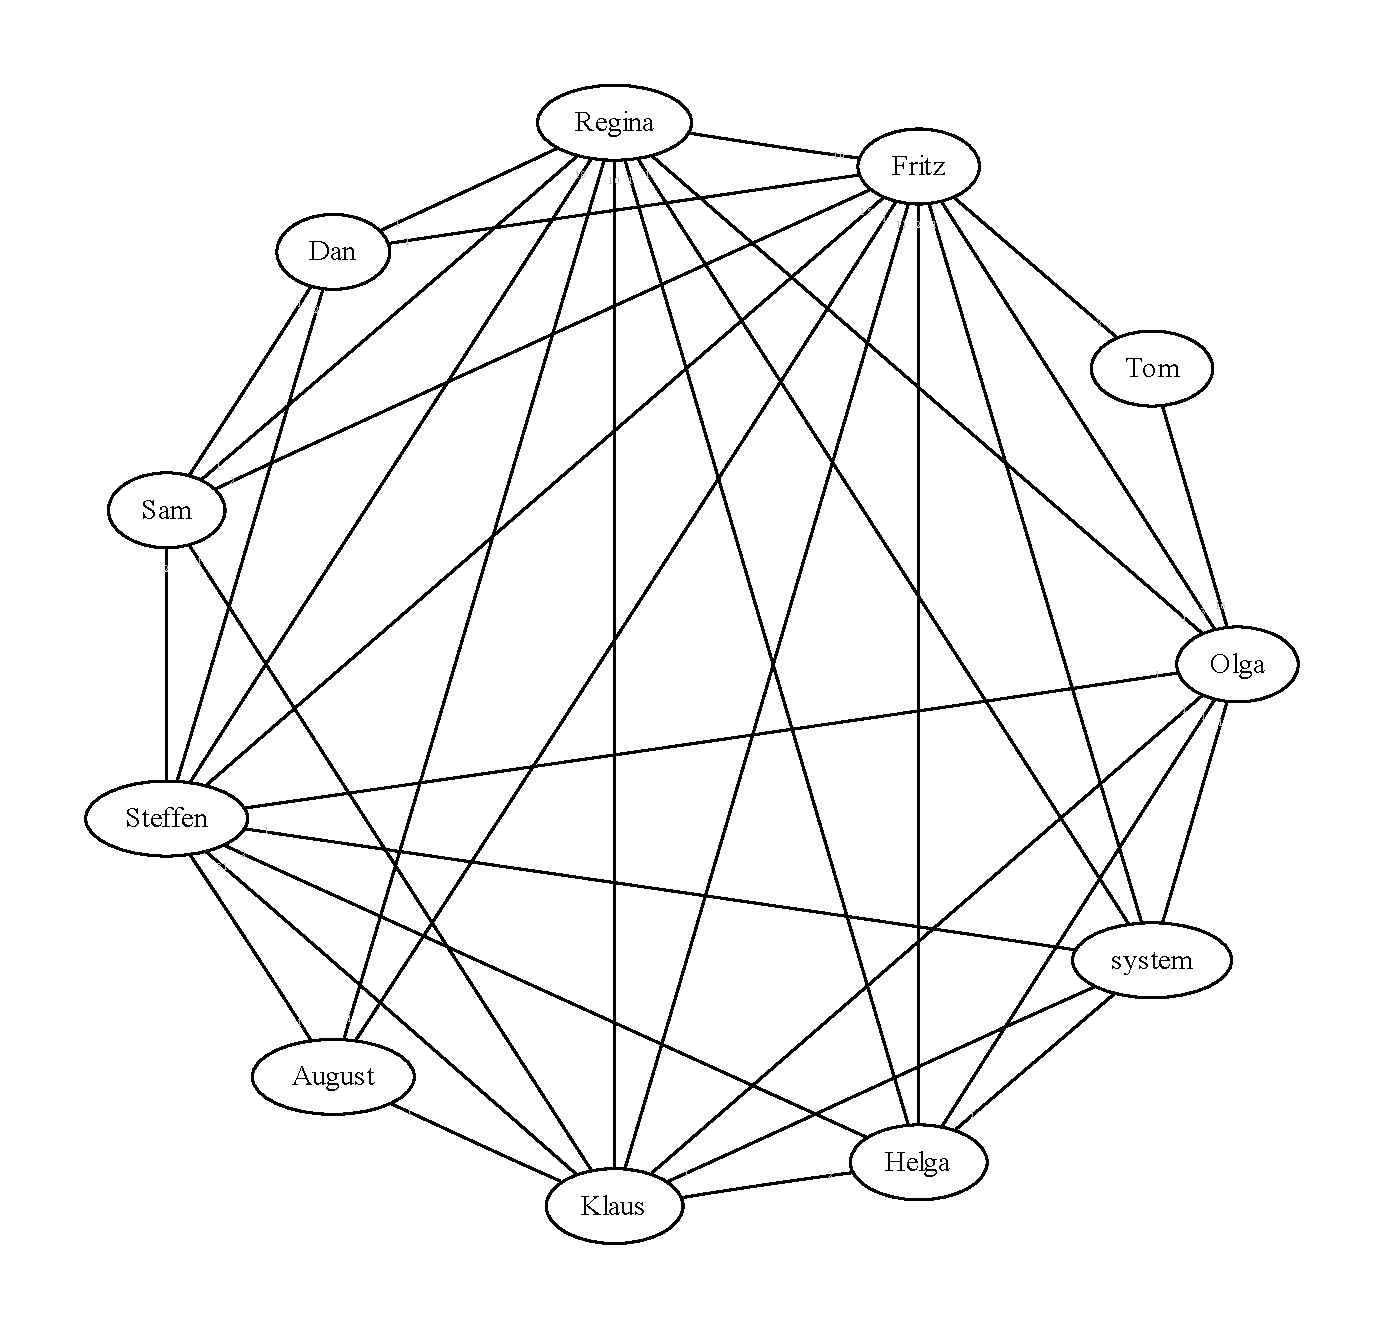
\includegraphics[width=\linewidth]{gv_ca-circo}\vspace{-7mm}
  \caption{\code{circo} layout}
  \label{fig:gv-cacirco}}%
\parbox[b]{0.3\textwidth}{\centering
  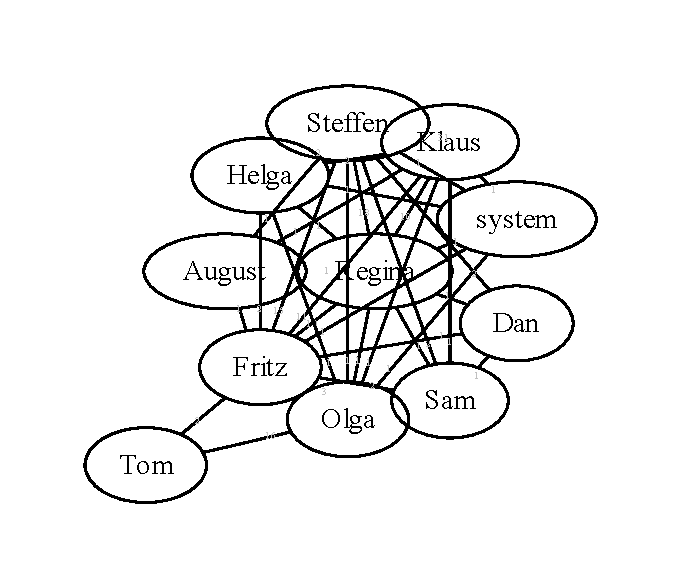
\includegraphics[width=\linewidth]{gv_ca-twopi}\vspace{-7mm}
  \caption{\code{twopi} layout}
  \label{fig:gv-catwopi}
  \vspace{8mm}

  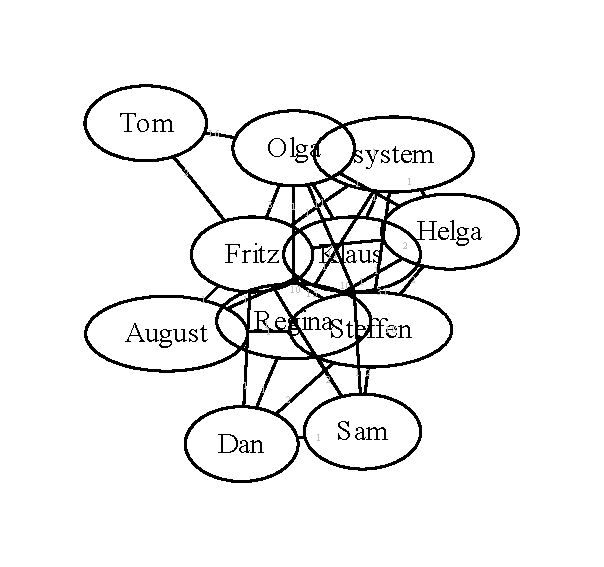
\includegraphics[width=\linewidth]{gv_ca-neato}\vspace{-7mm}
  \caption{\code{neato} layout}
  \label{fig:gv-caneato}}
\end{figure}

Network statistics are fine but we would rather be interested to see
some nice graphics. WikiExplorator can create graph visualizations in
different ways and with different layout algorithms using either
\file{graphviz} or \file{R}.

\subsubsection{Graphviz}
\label{sec:graphviz}

\file{graphviz} can be used in two ways: by default the graphviz
executables are called from ruby.\footnote{If you have the ruby gv library
installed you could require \file{util/dotgraph-gv.rb} for direct
library access. This is not done by default because of a graphviz bug
(reported and fixed since 2009-8-7).}
We start by using
different graphviz layout engines\footnote{see the \file{graphviz} manpage and
\url{http://www.graphviz.org/} for details} and create some PDFs:\footnote{(you may need to use \cmd{:pspdf} instead, see
  footnote~\ref{fnt:pspdf}, Sec.\,\ref{sec:gnuplot}), others
  (SVG, PNG, \dots) are available.}
\begin{typed}
\p{irb(main):107:0>} \c{cgraph.to_graphviz('gv_ca-dot.pdf','dot', :pdf)}
=> true
\p{irb(main):108:0>} \c{cgraph.to_graphviz('gv_ca-fdp.pdf','fdp', :pdf)}
=> true
\p{irb(main):109:0>} \c{cgraph.to_graphviz('gv_ca-circo.pdf','circo', :pdf)}
=> true
\p{irb(main):110:0>} \c{cgraph.to_graphviz('gv_ca-twopi.pdf','twopi', :pdf)}
=> true
\p{irb(main):111:0>} \c{cgraph.to_graphviz('gv_ca-neato.pdf','neato', :pdf)}
=> true
\end{typed}
This gives the graphs in figures~\ref{fig:gv-cadot}
to~\ref{fig:gv-caneato}.\footnote{These graphs as well as the
  statistics before do not include the unconnected nodes visible in
  figure~\ref{fig:coauthor} as we removed them in session~\ref{typed:remove_lonely_nodes}.}  These graphs obviously need some
finetuning. For the \code{twopi} (fig.\,\ref{fig:gv-catwopi}) and
\code{neato} (fig.\,\ref{fig:gv-caneato}) layout the nodes overlap,
and for \code{fdp}, \code{twopi} and \code{neato}
(fig.\,\ref{fig:gv-cafdp}--\ref{fig:gv-caneato}) the edges go across
the nodes. By passing additional parameters to graphviz we can solve
this (see the graphviz documentation for available options):

\begin{figure}
\parbox[b]{0.5\textwidth}{\centering
  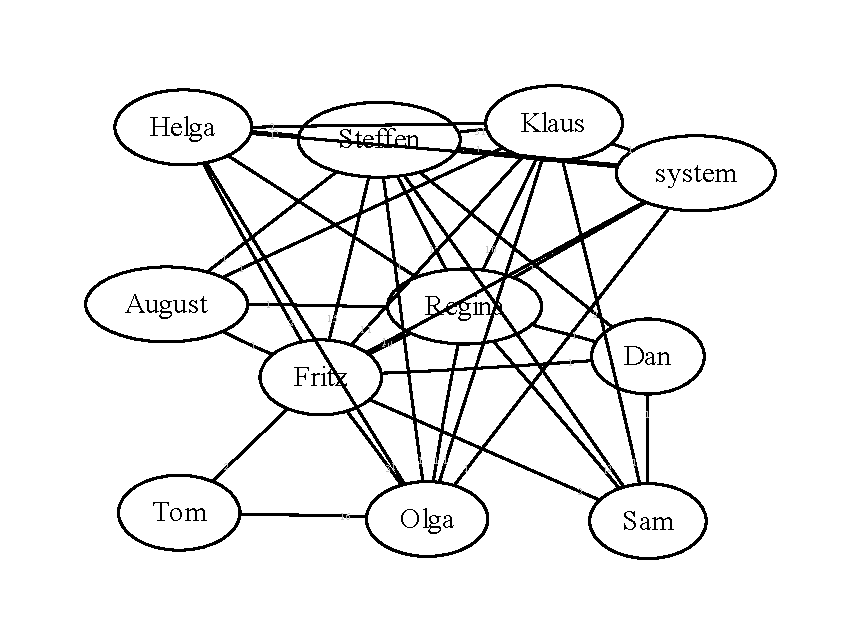
\includegraphics[width=\linewidth]{gv_ca-twopi-ol}\vspace{-1cm}
  \caption{\code{twopi} without overlap}
  \label{fig:gv-catwopi2}}%
\parbox[b]{0.5\textwidth}{\centering
  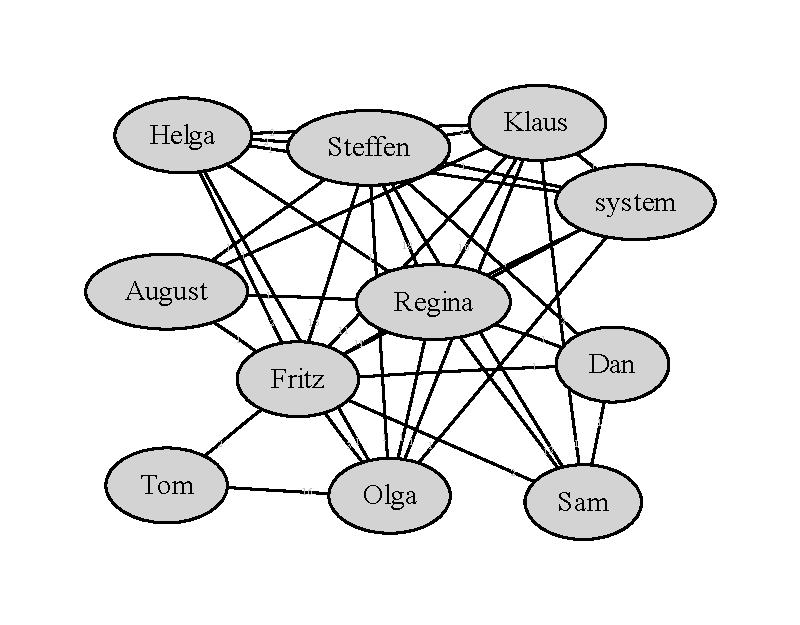
\includegraphics[width=\linewidth]{gv_ca-twopi-olf}\vspace{-1cm}
  \caption{\code{twopi}: nodes in front of edges}
  \label{fig:gv-catwopi3}}
\end{figure}

\begin{typed}
\p{irb(main):112:0>} \c{cgraph.to_graphviz('gv_ca-twopi-ol.pdf', 'twopi', :pdf, 
                                    'overlap=false')}
=> true
\p{irb(main):113:0>} \c{cgraph.to_graphviz('gv_ca-twopi-olf.pdf', 'twopi', :pdf, 
                                    'overlap=false', 'outputorder=edgesfirst', 
                                    'node [style=filled]')}
=> true
\end{typed}
The first call\footnote{\cmd{'overlap=false'} tells graphviz to shift
  the nodes apart from each other} gives figure~\ref{fig:gv-catwopi2},
the second\footnote{\cmd{'outputorder=edgesfirst'} tells graphviz to
  first draw the edges, so the nodes are printed over the edges. This
  only has an effect if the nodes are solid, so we add \cmd{'node
    [style=filled]'}} figure~\ref{fig:gv-catwopi3}. Try the same for
\code{fdp} and \code{neato}!
\begin{figure}
\parbox[b]{0.5\textwidth}{\centering
  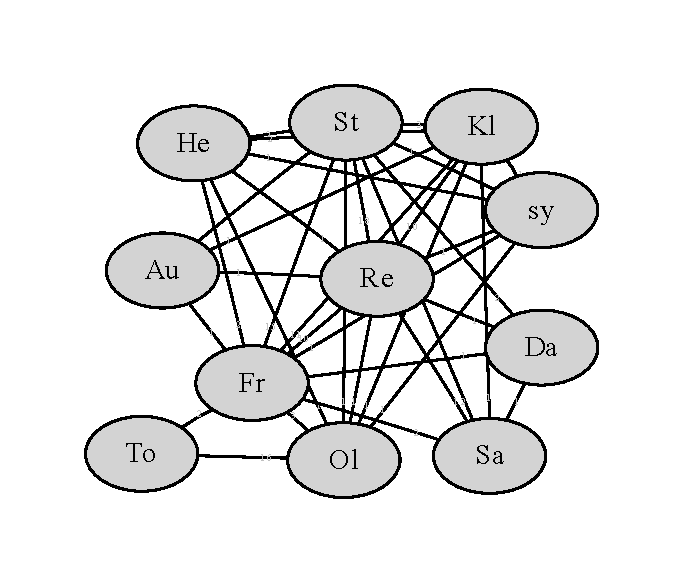
\includegraphics[width=\linewidth]{gv_ca-twopi-olf-short}
  \caption{\code{twopi}: short labels}
  \label{fig:gv-catwopi4}}%
\parbox[b]{0.5\textwidth}{\centering
  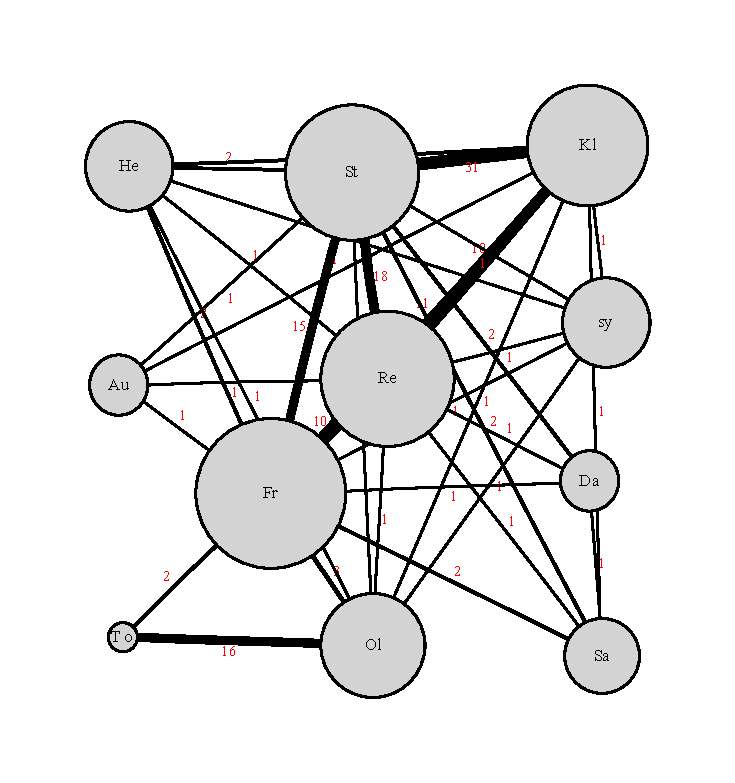
\includegraphics[width=\linewidth]{gv_ca-twopi-degwidth}\vspace{-1cm}
  \caption{\code{twopi}: weighted sizes}
  \label{fig:gv-catwopi5}}
\end{figure}
Currently the nodes have different size as the names (node labels) are
of different length. Perhaps we should abbreviate all labels to two
characters: 
\begin{typed}
\p{irb(main):115:0>} \c{cgraph.nodeblock \{ |node| node.name[0..1] \}}
=> #<Proc:0xf5ecf748@(irb):115>
\p{irb(main):116:0>} \c{cgraph.to_graphviz('gv_ca-twopi-olf-short.pdf', 'twopi', :pdf, 
                                    'overlap=false', 'outputorder=edgesfirst', 
                                    'node [style=filled]')}
=> true  
\end{typed}
In the first line we set the \code{nodeblock} of this graph. The
nodeblock is called for each node to create its label and should
either return a string (used as label) or an array (used as node
parameters). See \rdoc{DotGraph.nodeblock} for details.

I used this to create the hyperlink graph
(figure~\ref{fig:hyperlink}):
\begin{typed}
\p{irb(main):018:0>} \c{wiki.pagegraph \{''\}.to_graphviz('pagegraph.pdf', 'neato', :pdf, 
                     'outputorder=edgesfirst', 'overlap=false', 
                     'node [shape=note, style=filled, width=.34]')}
=> #<IO:0xf765e454>
\end{typed}
Here the nodeblock is given on creation and returns an empty string
for any node. By adding some width and shape directives I got these
nice paper icons as node shapes to represent our wiki pages.

And for completeness, here is figure~\ref{fig:coauthor} (we create a
new coauthorgraph from the wiki, so here the unconnected nodes are not
removed and therefore displayed in the graph):
\begin{typed}
\p{irb(main):028:0>} \c{wiki.coauthorgraph.to_graphviz('gv_coauthorgraph-full.pdf',
                     'neato', :pdf, "outputorder=edgesfirst", "overlap=false", 
                     "node [style=filled]")}
=> #<IO:0xf7a7554c>
\end{typed}

Finally, we want to compute node sizes dependent on node degrees and
edge width dependent on link weights\footnote{\cmd{coauthorgraph}
  weights edges between authors with the number of pages they are
  coauthors on.}:
\begin{typed}
\p{irb(main):161:0>} \c{cgraph.nodeblock \{ |node| 
                                    size = (cgraph.n_degree(node)/10.0).to_s; 
                                    ["label=#\{node.name[0..1]\}", 
                                     'width=' + size, 'height=' + size] \}}
=> #<Proc:0xf5c80dd4@(irb):161>
\p{irb(main):173:0>} \c{cgraph.to_graphviz('gv_ca-twopi-degwidth.pdf', 'twopi', :pdf, 
                     'overlap=false', 'outputorder=edgesfirst',
                     'node [fontsize=8, style=filled, fixedsize]') \{ |weight| 
                        ["penwidth=#\{weight**0.5\}", "label=#\{weight\}", 
                         'fontsize=7', 'fontcolor=red' ] \}}
Warning: node 'u6', graph 'G' size too small for label
Warning: node 'u12', graph 'G' size too small for label
Warning: node 'u15', graph 'G' size too small for label
=> #<IO:0xf5bb9950>
\end{typed}
We first set the nodeblock. We use the degree of the node to compute
the \cmd{size}: we ask \cmd{cgraph} for the degree of the node and
divide it by 10.0.\footnote{the divisor has to be a Float, otherwise
  ruby would use Integer division} The method \cmd{to\_s} converts the
result to string. Now we asseble an array with three entries: the node
label set to the first two characters of the user name, the node width
and the node height, both set to \cmd{size}.\footnote{You may notice
  usage of single (\cmd{'}) and double (\cmd{"}) quotes. This is
  similar to shells like sh or bash: strings in double quotes
  (\cmd{"}) are subject to substitution, in our example this means
  that the result of the ruby code given in \cmd{\#\{\dots\}} is
  inserted in the string.}  And finally we ask \cmd{cgraph} to create
the graph. You may notice that we appended an additional block to this
call. This block is called for each edge with the edge weight as
parameter, similar to nodeblock.

Graphviz allows much more than the few examples shown
here,\footnote{see the gallery at
  \url{http://www.graphviz.org/Gallery.php}}, if you find expressive
and impressive visualizations feel free to send me examples (source
code and graphics). The parameters are described at
\url{http://www.graphviz.org/doc/info/attrs.html}, the graphviz
homepage provides elaborate user manuals for all layout
algorithms. Use \cmd{to\_dotfile} to see the outcome of the parameters:
\begin{typed}
\p{irb(main):218:0>} \c{cgraph.to_dotfile('cgraph.dot', 'outputorder=edgesfirst',
                     'overlap=false', 'node [style=filled]')  \{ |weight| 
                            ["penwidth=#\{weight**0.5\}", "label=#\{weight\}"] \}}
=> #<File:~/mwparser/cgraph.dot (closed)>
\end{typed}
The resulting file \file{cgraph.dot} can be opened with any text editor.

%WikiExplorator may write graphs in \code{dot} format you can also
%use these to directly experiment with the graphviz toolbox.

Lets close with one final example. We use (nearly) the same parameters
as before and just change the layout engine (figure~\ref{fig:gv-catcirco}):
\begin{figure}[t]
  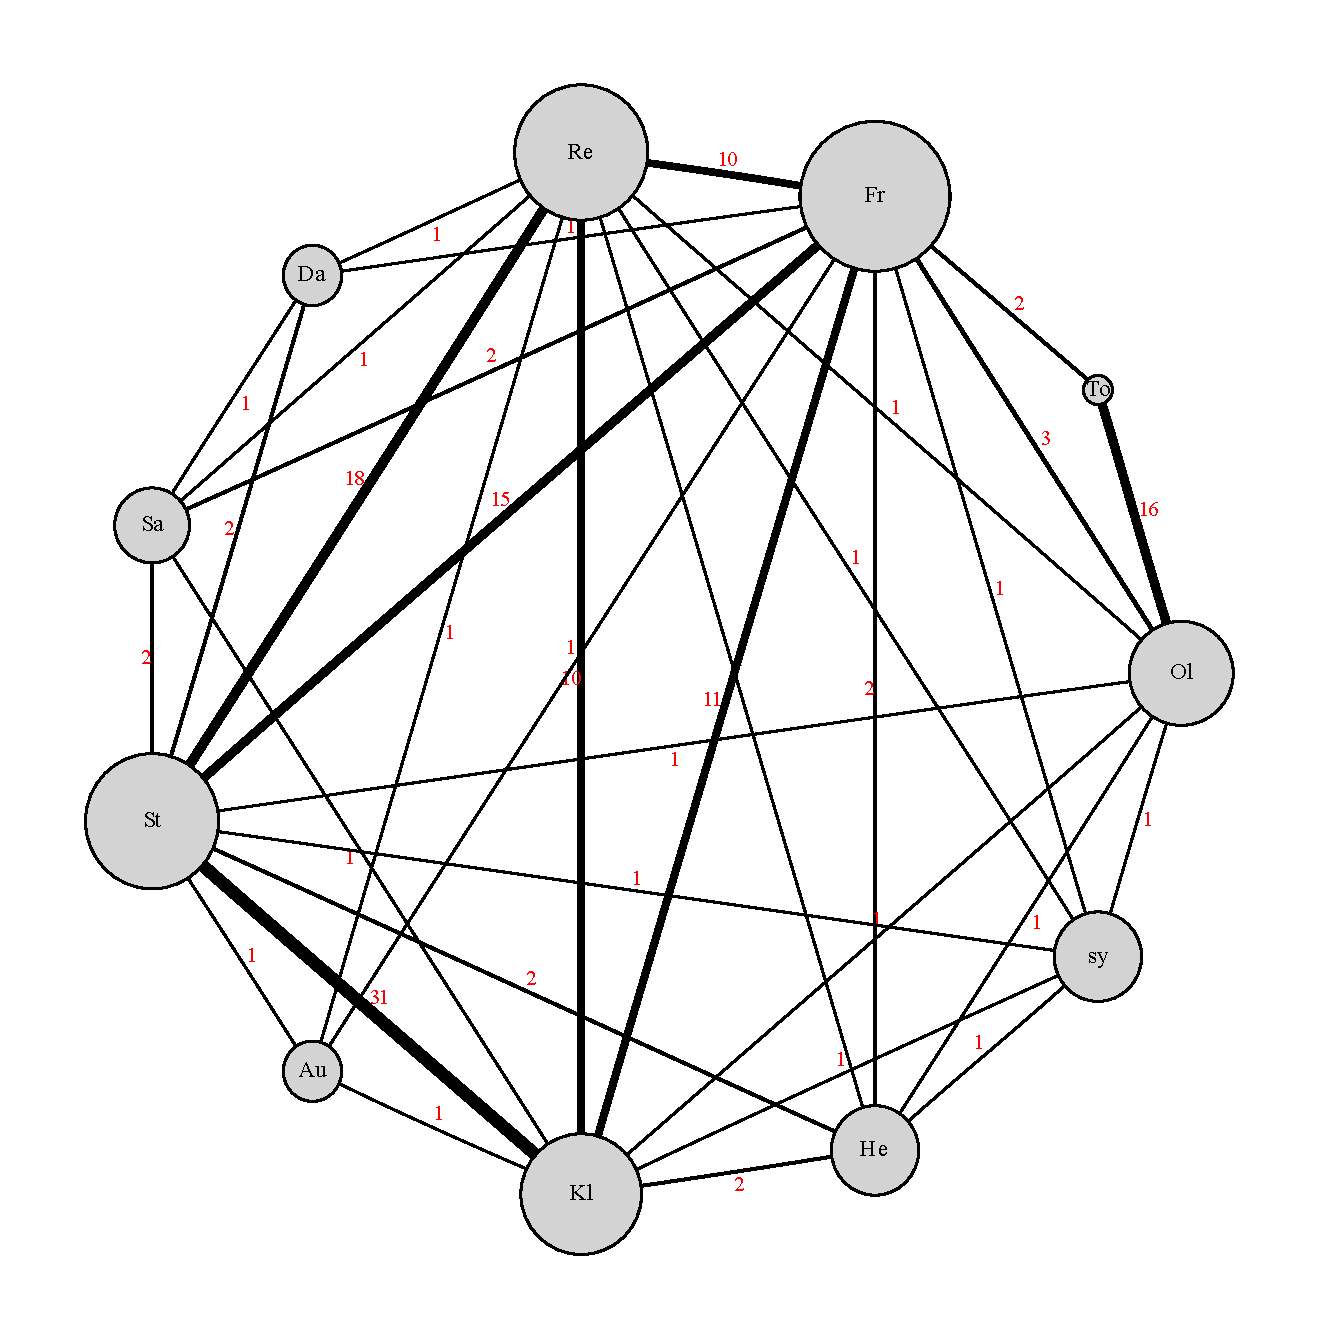
\includegraphics[width=\linewidth]{gv_ca-circo-degwidth}\vspace{-1cm}
  \caption{\code{circo}: weighted sizes}
  \label{fig:gv-catcirco}
\end{figure}
\begin{typed}
\p{irb(main):180:0>} \c{cgraph.to_graphviz('gv_ca-circo-degwidth.pdf', 'circo', :pdf, 
                     'overlap=false', 'outputorder=edgesfirst', 
                     'node [fontsize=11, style=filled, fixedsize]')  \{ |weight|
                        ["penwidth=#\{weight**0.5\}", "label=#\{weight\}", 
                         'fontsize=10', 'fontcolor=red' ] \}}
Warning: node 'u6', graph 'G' size too small for label
Warning: node 'u12', graph 'G' size too small for label
Warning: node 'u15', graph 'G' size too small for label
=> #<IO:0xf5b7fc00>
\end{typed}

\subsubsection{R}
\label{sec:vizR}

Graphviz allows for rather pretty and sophisticated graph prints, but
has the drawback not to display graphs on screen (which was rather
convenient with gnuplot). Thankfully we can use \code{R} for this
(figure~\ref{fig:r_coauthor}):
\begin{typed}
\p{irb(main):182:0>} \c{dev = cgraph.r_plot}
=> 2
\p{irb(main):183:0>} \c{cgraph.r_plot_close(dev)}
=> {"null device"=>1}
\end{typed}
\begin{figure}
  \parbox[b]{0.37\textwidth}{%
    \centering
    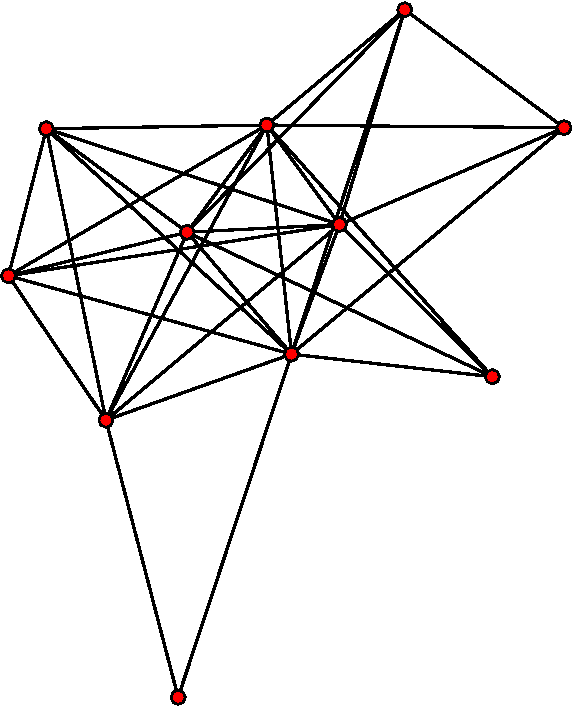
\includegraphics[width=\linewidth]{r_coauthor}
    \caption{Plotting using \code{R}}
    \label{fig:r_coauthor}
  }
  \parbox[b]{0.63\textwidth}{%
    \centering
    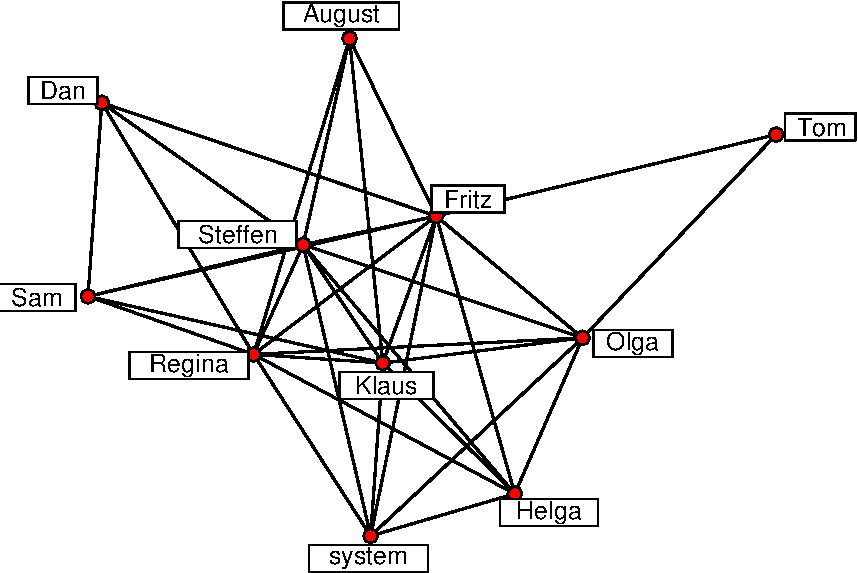
\includegraphics[width=\linewidth]{r_coauthor2}
    \caption{Plotting with labels using \code{R}}
    \label{fig:r_coauthor2}
  }
\end{figure}
As you can see \cmd{cgraph.r\_plot} returns a number which indicates
the \code{R} plot device and which can be used to close the graph
window. On some OS you may just close the window using its close
button, on others this does not work, there you have to use
\cmd{r\_plot\_close}.

Unfortunately changing attributes can get somehow cumbersome using
\code{R} syntax, well, at least for me, if you know \code{R} from
heart things may be different for you
(figure~\ref{fig:r_coauthor2}):\footnote{this example uses
  \cmd{DotGraph.r\_plot\_close} which works as well and ist independent
  of a certain graph object.}
\begin{typed}
\p{irb(main):190:0>} \c{cgraph.r_plot(:displaylabels => TRUE,
                     :label => lambda \{ |nw,r| 
                        r.get_vertex_attribute(nw, "attr")\}) \{ |u| u.name \}}
=> 2
\p{irb(main):191:0>} \c{DotGraph.r_plot_close(2)}
=> {"null device"=>1}
\end{typed}
So I use \cmd{r\_plot} for a fast interactive graph overview and stay
with graphviz for prints.

\section{Using Filters}
\label{sec:filters}

Enough of playing with graphs and networks, back to the wiki.

As stated before the wiki is not seen raw but through a view which is
customized by a filter. Filters are the way to see cutouts of a wiki,
including or excluding certain users, namespaces, and to go back in
time, to see how the wiki looked like years ago or what happened
within a certain timespan.

\subsection{First steps}
\label{sec:filters-first}

When asking the wiki for the number of pages by default I only get
pages from the main namespace (0). But we certainly can change this:
\begin{typed}
\p{irb(main):199:0>} \c{wiki.pages.length}
=> 109
\p{irb(main):200:0>} \c{wiki.filter.include_all_namespaces}
=> #<Set: {0, 6, 1, 2, 8, 14, 3, 4, 10}>
\p{irb(main):201:0>} \c{wiki.pages.length}
=> 271
\end{typed}
We first ask the wiki for its pages. After that \cmd{wiki.filter}
gives us the active filter of the wiki on which we call the method
\cmd{include\_all\_namespaces}. As we can see from the return value
this automagically collects all namespaces found in the wiki. And
finally we ask the wiki again for its pages, and suddenly their number
raises from 109 to 271.
\bigskip

We have two users in our wiki who are not part of our normal staff:
``system'' and ``WikiSysop''.\footnote{While the ``WikiSysop'' is an
  ordinary wiki user with special rights, the ``system'' user is
  special. It does not show up in the user database and you cannot
  login as ``system'' user, but it is owner of all revisions done
  internally by Mediawiki (e.\,g. as result of mass uploads etc.).  }
Perhaps we should exclude them from our statistics:
\begin{typed}
\p{irb(main):230:0>} \c{f = wiki.filter}
=> #<Mediawiki::Filter:0xf7669e6c ...>
\p{irb(main):231:0>} \c{wiki.revisions.length}
=> 1362
\p{irb(main):232:0>} \c{wiki.user_by_name('system').revisions.length}
=> 2
\p{irb(main):233:0>} \c{wiki.user_by_name('WikiSysop').revisions.length}
=> 1
\p{irb(main):234:0>} \c{f.deny_user('system', 'WikiSysop')}
=> ["system", "WikiSysop"]
\p{irb(main):235:0>} \c{wiki.revisions.length}
=> 1359
\end{typed}
We ask the wiki for its filter and save it in \cmd{f}. The wiki
currently has 1362 revisions, the ``system'' user has two revisions
and ``WikiSysop'' has one. Now we tell the filter to exclude these two
users and the wiki shows us 1359 ($=1362-2-1$) revisions, so this
looks fine.

\bigskip

How does this work? Well, when we ask the wiki for its users, we get a
UsersView of the wiki which uses the given filter:
\begin{typed}
\p{irb(main):240:0>} \c{users = wiki.users}
=> #<Mediawiki::UsersView:0xf5d4dba4 ...>
\p{irb(main):241:0>} \c{users.length}
=> 13
\p{irb(main):242:0>} \c{f.undeny_user('WikiSysop')}
=> ["WikiSysop"]
\p{irb(main):243:0>} \c{users.length}
=> 14
\end{typed}
What we see here is that changing the filter affects the corresponding
view.


\subsection{Multiple Filters}
\label{sec:filter-dup}

In the last section we changed the current filter of the wiki to get
different views. This does not work if we want to deal with different
views in parallel: we need more than one filter. So let's copy our
current filter and see what we can do with it:
\begin{typed}
\p{irb(main):244:0>} \c{f2 = f.clone}
=> #<Mediawiki::Filter:0xf5d43618 ...>
\p{irb(main):245:0>} \c{f2.namespace = 0}
=> 0
\p{irb(main):246:0>} \c{wiki.revisions(f2).length}
=> 1124
\p{irb(main):247:0>} \c{wiki.revisions.length}
=> 1360
\end{typed}
We use \cmd{clone} to get a real copy of the filter \cmd{f} and save
it in \cmd{f2},\footnote{cloning is important, otherwise both
  varfiables would point to the \emph{same} object!} after that we
restrict the namespace of \cmd{f2} to 0 and then we use \cmd{f2} for
the \cmd{revisions} view. Many Wiki methods\footnote{i.\,e. graph
  generation and statistics methods} take a filter as optional
parameter.\footnote{send a bug report if I missed a method.}

A cloned filter inherits the attributes of the original
one. Alternatively we can create a clean filter for our wiki:
\begin{typed}
\p{irb(main):249:0>} \c{f3 = Mediawiki::Filter.new(wiki)}
=> #<Mediawiki::Filter:0xf5cf2628 ...>
\end{typed}
So \cmd{f3} has all attributes set to start values (namespace 0, no
excluded users, \dots).

See \rdoc{Mediawiki::Filter} to learn about filter attributes.

\subsection{Back and Forth in Time}
\label{sec:filter-time}

One nice feature of a wiki is the page history. We can reconstruct how
the wiki looked like months or years ago,\footnote{WikiExplorator
  currently does not handle deleted pages, this is considered a bug.}
and we do this using filters.

So let's see how the wiki looked like a year ago:
\begin{typed}
\p{irb(main):260:0>} \c{f3.revision_timespan}
=> Di Mär 20 18:23:15 UTC 2007..Di Jul 28 13:53:09 UTC 2009
\p{irb(main):261:0>} \c{f3.endtime = '2008-8-1'}
=> "2008-8-1"
\p{irb(main):262:0>} \c{f3.revision_timespan}
=> Di Mär 20 18:23:15 UTC 2007..Fr Aug 01 00:00:00 +0200 2008
\p{irb(main):266:0>} \c{wiki.pages(f3).length}
=> 84
\p{irb(main):268:0>} \c{wiki.pages(f2).length}
=> 109
\end{typed}
Initially \cmd{f3} includes the whole timespan from March 20, 2007 to
July 28, 2009. We set the endtime to August 1, 2008 and ask again for
the timespan, fine, worked like expected.

Now we ask the wiki for the pages within this timespam (84) and
compare it to the number of pages until now (109). So obviously we got
25 ($=109-84$) new pages added in the last year.

Ok, how many revisions within the last four weeks?
\begin{typed}
\p{irb(main):270:0>} \c{f3.full_timespan}
=> Di Mär 20 18:23:15 UTC 2007..Di Jul 28 13:53:09 UTC 2009
\p{irb(main):271:0>} \c{f3.starttime = f3.endtime - 60*60*24*7*4}
=> Di Jun 30 13:53:09 UTC 2009
\p{irb(main):272:0>} \c{f3.revision_timespan}
=> Di Jun 30 13:53:09 UTC 2009..Di Jul 28 13:53:09 UTC 2009
\p{irb(main):273:0>} \c{wiki.revisions(f3).length}
=> 10
\end{typed}
We first set \cmd{f3} to full timespan, set the new starttime by
subtracting four weeks in seconds from the endtime, controlled that it
worked and asked for the number of revisions. Not much traffic in our
example wiki the last four weeks.

Wouldn't it be nice to have this for the whole timeline? That's easy
as the wiki helps us generating a custom timeraster:
\begin{typed}\label{typed:revtr}
\p{irb(main):270:0>} \c{f3.full_timespan}
=> Di Mär 20 18:23:15 UTC 2007..Di Jul 28 13:53:09 UTC 2009
\p{irb(main):275:0>} \c{tr = wiki.timeraster(:step => :week, :zero => :week)}
=> [So Mär 18 00:00:00 +0100 2007, So Mär 25 00:00:00 +0100 2007, ...,
                                     ..., So Aug 02 01:00:00 +0200 2009]
\p{irb(main):279:0>} \c{ r1 = tr.collect \{ |t| f3.endtime = t; 
                                        [t, wiki.revisions(f3).length] \}}
=> [[So Mär 18 00:00:00 +0100 2007, 0], [So Mär 25 00:00:00 +0100 2007, 18], ...,
                                     ..., [So Aug 02 01:00:00 +0200 2009, 1125]]
\p{irb(main):284:0>} \c{r1.gp_plot(:with => 'lines'); nil}
=> nil
\end{typed}
First we reset \cmd{f3} to full timespan (again). Then we ask the wiki
to generate a weekly timeraster and use this timeraster to compile an
array of arrays with the endtime as first and the number of revisions
up to this time as second entry. And finally we use gnuplot to plot
the revision growth in time (figure~\ref{fig:gp_revtr}).

\begin{figure}
  \parbox[b]{.5\textwidth}{%
  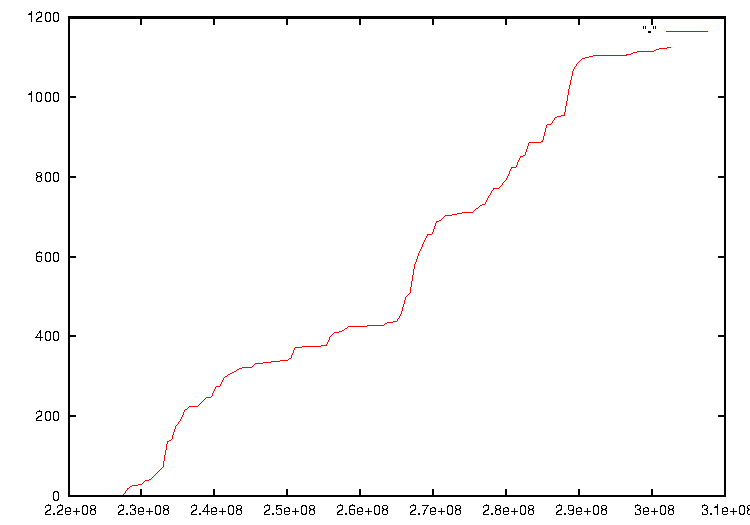
\includegraphics[width=\linewidth]{gp_revtr}
  \caption{weekly revisions (cumulative)}
  \label{fig:gp_revtr}}
  \parbox[b]{.5\textwidth}{%
  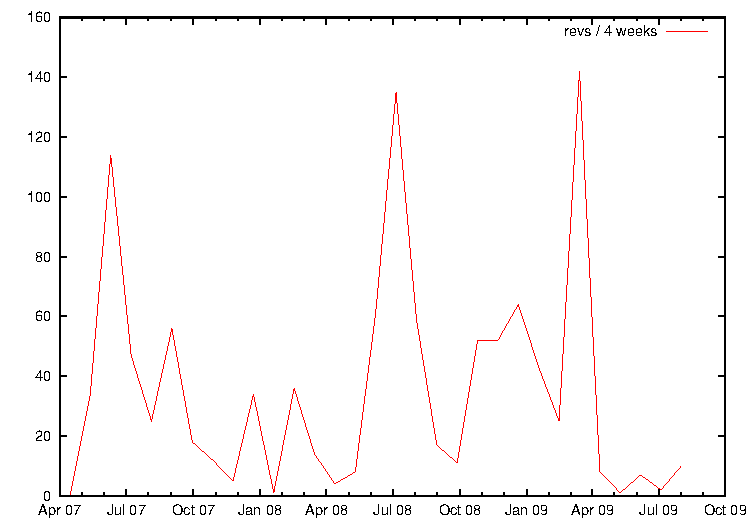
\includegraphics[width=\linewidth]{gp_revtr2}
  \caption{monthly revisions}
  \label{fig:gp_revtr2}}
\end{figure}

In the last example we only changed endtime, so the number of
revisions grew. Now we want to see how the number of new revisions
changes in time. The following example could be written slightly more
simple when using the \file{enumerator} module available in ruby 1.8.7
and later (see \rdoc{Mediawiki::Wiki.timeraster} for an example using
enumerator). We use a time raster of four weeks:
\begin{typed}
\p{irb(main):339:0>} \c{tr = wiki.timeraster(:step => 60*60*24*7*4, :zero => :week)}
=> [So Mär 18 00:00:00 +0100 2007, So Apr 15 01:00:00 +0200 2007, ...]
\p{irb(main):340:0>} \c{start = tr.shift}
=> So Mär 18 00:00:00 +0100 2007
\p{irb(main):341:0>} \c{r2 = tr.collect \{ |t| f3.revision_timespan = (start..t); 
                                       start = t; 
                                       [t, wiki.revisions(f3).length] \}}
=> [[So Apr 15 01:00:00 +0200 2007, 0], ... ]
\p{irb(main):381:0>} \c{Gnuplot.new do |gp|}
\p{irb(main):382:1*} \c{  gp.set('xdata', 'time')}
\p{irb(main):383:1>} \c{  gp.set('timefmt', '%Y-%m-%d', true)}
\p{irb(main):384:1>} \c{  gp.set('format x', '%b %y', true)}
\p{irb(main):385:1>} \c{  gp.add(r2, :with => 'lines', :title => 'revs / 4 weeks',
                              :timefmt => '%Y-%m-%d')}
\p{irb(main):386:1>} \c{  gp.plot}
\p{irb(main):387:1>} \c{end}
=> #<Gnuplot:0xf5d8a61c ...>
\end{typed}
As you can see I put some efforts in gnuplot to get nice formatted output.
So I hope you got an idea about what filters can do for you, even if
sometimes the direct way is faster (this results in a graph very close
to session~\ref{typed:revtr} (figure~\ref{fig:gp_revtr})):
\begin{typed}
\p{irb(main):416:0>} \c{c = 0; wiki.revisions.sort_by \{ |r| r.timestamp \}.collect \{ |r| 
                             [r.timestamp, c += 1] \}.gp_plot(:with => 'lines')}
\end{typed}
Here we directly use the revision timespans to generate the graph.

\section{Load and Save}
\label{sec:load}

Until now we played with a wiki we loaded directly from the database
(we come back to this at the end of this section,
see~\ref{sec:Wiki.open}). 

\subsection{Loading and Dumping}
\label{sec:loaddump}

Sometimes it would be nice to take the wiki with us to be able to do some
statistics, reporting, working through this tutorial etc. on our
laptop while sitting in the train without internet access. To support
this we can dump the wiki on disk to load it later.

\subsubsection{Remove Sensible Data}
\label{sec:obliterate}

Taking a wiki with us means dumping wiki contents on our hard
disk. You may want to analyze the wiki of your customer containing
sensible data, and you may want to take it with you on your laptop,
but your customer would not like to see sensible data leaving the
intranet.

As we nearly do not need the contents of the wiki pages for most
analyses the \cmd{obliterate} method is our friend. This method
removes page contents, user names, page titles etc. from the wiki and
keeps only the structure which is enough to do nearly anything we want
(except for text corpus and text size analysis):
\begin{typed}
\p{irb(main):471:0>} \c{page = wiki.page_by_id(1)}
=> #<Mediawiki::Page id=1 title="Hauptseite">
\p{irb(main):472:0>} \c{page.content}
=> "'''Wikis in Organizations''' ..."
\p{irb(main):473:0>} \c{wiki.obliterate}
=> #<Mediawiki::Wiki WiO: wiowiki.kinf.wiai.uni-bamberg.de/wiodb,
\hfill 271 pages, 1362 revisions, 15 users>
\p{irb(main):474:0>} \c{page.content}
=> ""
\p{irb(main):475:0>} \c{page}
=> #<Mediawiki::Page id=1 title="p1">
\end{typed}
What exactly is removed/kept by \cmd{obliterate} is freely selectable
by the user (see \rdoc{Mediawiki::Wiki.obliterate} for details).

\subsubsection{Marshal Dump and Load}
\label{sec:marshal}

Now we can dump our wiki to disk for later usage:
\begin{typed}
\p{irb(main):478:0>} \c{wiki.marshal_save('wio.marshal')}
=> #<File:~/mwparser/wio.marshal (closed)>
\p{irb(main):479:0>} \c{exit}
\end{typed}%
We leave irb, have a break, meet people and do real world stuff, you
know, things that really matter, thinks you don't need a computer for, and
later we come back and start again, now loading our wiki from
file:\footnote{``\cmd{-r wio}'' is needed to pull in the
  WikiExplorator library. As we do not need a customized database
  connector we could also have used ``\cmd{-r mediawiki/full}'' instead.}
\begin{typed}
\p{~/mwparser/>} \c{irb -r wio}
...
\p{irb(main):001:0>} \c{wiki = Mediawiki::Wiki.marshal_load('wio.marshal')}
MARSHAL load...
done
=> #<Mediawiki::Wiki WiO: wiowiki.kinf.wiai.uni-bamberg.de/wiodb,
\hfill 271 pages, 1362 revisions, 15 users>\quad
\end{typed}

I have obliterated marshal dumps of all of the wikis I am working on
and use only these for daily work.\footnote{this has the nice
  side effect that it works on platforms where installing a
  Mysql connector gets laborious.}

\subsubsection{YAML Dump and Load}
\label{sec:yaml}

Marshalling is fast and reliable, but it dumps the wiki to some binary
format, so your customer cannot control what data you want to take
with you. YAML is much slower than marshal but writes human readable
files so you can show them what you want to take away:
\begin{typed}
\p{irb(main):002:0>} \c{wiki.yaml_save('wio.yaml')}
preprocessing (detach links)...
YAML save (may take some time)...
postprocessing (attach links)...
done
=> #<Mediawiki::Wiki WiO: wiowiki.kinf.wiai.uni-bamberg.de/wiodb, 
\hfill 271 pages, 1362 revisions, 15 users>
\p{irb(main):004:0>} \c{exit}
\end{typed}
This time we do some sports before we come back. Oh, and have a look
into ``\file{wio.yaml}'' to see what's inside (figure~\ref{fig:yaml})
\begin{typed}
\p{~/mwparser/>} \c{irb -r wio}
...
\p{irb(main):001:0>} \c{wiki = Mediawiki::Wiki.yaml_load('wio.yaml')}
YAML load...
postprocessing (attach links)...
done
=> #<Mediawiki::Wiki WiO: wiowiki.kinf.wiai.uni-bamberg.de/wiodb,
\hfill 271 pages, 1362 revisions, 15 users>\quad
\end{typed}
YAML is an ordinary ruby library, but as you can see by the messages
above I had to provide a customized version as yaml has problems with
large nested cyclic structures. So please only use the methods given
above to YAML save and load your wiki and not the original ones
privided by the YAML lib.

\begin{figure}
  \centering
  \begin{File}\footnotesize
--- &id001 !ruby/object:Mediawiki::Wiki 
dburl: wiowiki.kinf.wiai.uni-bamberg.de/wiodb
filter: !ruby/object:Mediawiki::Filter 
  revision_timespan: !ruby/range 
    begin: &id002 2007-03-20 19:23:15 +01:00
    end: &id003 2009-07-28 15:53:09 +02:00
    excl: false
  ...
language: de
name: WiO
...
pages_id: 
  1440: !ruby/object:Mediawiki::Page 
    len: 864
    namespace: 0
    pid: 1440
    ...
  1641: !ruby/object:Mediawiki::Page 
    ...
  ...
pages_title: 
  ...
revisions_id: 
  1556: !ruby/object:Mediawiki::Revision 
    page: 1425
    rid: 1556
    text: 1556
    timestamp: &id156 2007-05-23 13:26:52 +02:00
    user: 5
    ...
  2405: !ruby/object:Mediawiki::Revision 
    ...
  ...
texts_id: 
  1823: !ruby/object:Mediawiki::Text 
    text: ""
    tid: 1823
    ...
  ...
users_id: 
  5: !ruby/object:Mediawiki::User 
    name: u5
    revisions: 
      ...
    uid: 5
    ...
  0: !ruby/object:Mediawiki::User 
    ...
  ...
users_name: 
  ...
version: 1.8
\end{File}\vspace{-\topskip}
  \caption{YAML dump of the wiki (excerpt)}
  \label{fig:yaml}
\end{figure}

\subsection{Wiki.open}
\label{sec:Wiki.open}

At the beginning of this tutorial (section~\ref{sec:start}) we
created our Wiki object by adapting some values in \file{mywikis.rb}. 
We could have done this directly:
\begin{typed}
\p{~/mwparser/>} \c{irb -r mediawiki/full}
...
\p{irb(main):001:0>} \c{wiki = Mediawiki::Wiki.open("wiodb", 
\hfill "wiowiki.kinf.wiai.uni-bamberg.de", "wiouser", 'secret',
\hfill :language => 'de', :name => 'WiO')}
connecting to database wiowiki.kinf.wiai.uni-bamberg.de/wiodb
...
Done.
=> #<Mediawiki::Wiki WiO: wiowiki.kinf.wiai.uni-bamberg.de/wiodb, 
\hfill 271 pages, 1362 revisions, 15 users>\quad
\end{typed}
Using a startup file is just convenient. 

Please have a detailed look at \rdoc{Mediawiki::Wiki.open} (and
\rdoc{Mediawiki::DB.new}) in the manual for the various parameters. It
is important to set the right wiki name, the right language and give
mappings for additional namespaces to get correct link structures.

Mediawiki unfortunately does not put everything into the database,
the correct interpretation of various data depends on the values in
\file{Localsettings.php}, so I had no choice than to give these as
parameter. 

Two of the parameters allow special customation: \cmd{:ips} and
\cmd{:uid\_aliases}.

\subsubsection{:ips}
\label{sec:ips}

If a wiki allows anonymous edits the IP address of the editing
anonymous user is saved for each revision. Normally it is not useful
to distinguish between different IPs as the same user may come back
with a different IP the next day (at least if he has a dialup
connection to the internet), so all anonymous edits are mapped to one
default IP user.

Within an intranet things may different as the workstations of the
staff may have fixed IP addresses. In this case simply add ``\cmd{:ips
=> true}'' to the parameters and a new user is created for each IP.

\subsubsection{:uid\_aliases}
\label{sec:uid_aliases}

On many of the wiki we analyzed we found users with more than one
login, either because login name policy of the company changed after
the wiki started or users sometimes logged in and sometimes forgot and
did anonymous edits from a fixed IP address etc.\footnote{we even had
  a company where we could map sets of IP addresses to certain roles
  but not one IP address to one user.}

To deal with these situations WikiExplorator allows to merge
users. For example, in our example wiki I know that ``WikiSysop'' and
``Klaus'' are the same person, so we may want to merge
them\footnote{on the other hand it may be a bad idea, but, well, we do
  it to have an example.}:
\begin{typed}
\p{irb(main):002:0>} \c{wiki.user_by_name('Klaus')}
=> #<Mediawiki::User id=2 name="Klaus">
\p{irb(main):003:0>} \c{wiki.user_by_name('WikiSysop')}
=> #<Mediawiki::User id=1 name="WikiSysop">
\p{irb(main):004:0>} \c{wiki = Mediawiki::Wiki.open("wiodb", 
                    "wiowiki.kinf.wiai.uni-bamberg.de", "wiouser", 'secret',
                    :language => 'de', :name => 'WiO', :uid_aliases => \{1 => 2\})}
connecting to database wiowiki.kinf.wiai.uni-bamberg.de/wiodb
connected.
Table wio_genres in DB not found
Table wio_roles in DB not found
...
Done.
=> #<Mediawiki::Wiki WiO: wiowiki.kinf.wiai.uni-bamberg.de/wiodb, 
\hfill 271 pages, 1362 revisions, 14 users>
\p{irb(main):017:0>} \c{wiki.user_by_id(1)}
=> nil
\end{typed}
It worked. We first looked up the ids of ``Klaus'' and ``WikiSysop''
and then opened the wiki aliasing 1 to 2. All revisions of user 1 now
belong to user 2.

\subsubsection{wio\_roles and wio\_genres}
\label{sec:wioroles}

\begin{figure}
  \parbox[b]{.5\textwidth}{\centering
  \begin{tabular}{rll}\toprule
    \multicolumn{2}{l}{\code{page\_id}} & \code{genres}\\\midrule
    1 && portal\\
    1410 && description>project\\
    1424 && list>todo\\
    1471 && list>collection, article\\
    1477 && howto, article\\
    1554 && description>project\\
    1623 && calendar, event\\
    && \dots\\
    \bottomrule
  \end{tabular}
  \caption{\code{wio\_genres} table}
  \label{fig:wio_genres}}
  \parbox[b]{.5\textwidth}{\centering
  \begin{tabular}{rll}\toprule
    \multicolumn{2}{l}{\code{user\_id}} & \code{roles}\\\midrule
     2 && Support\\
     4 && Staff\\
     5 && ProjectManagement\\
     6 && ProjectManagement\\
     7 && Staff\\
     8 && Interns\\
    10 && Interns\\
    && \dots\\
    \bottomrule
  \end{tabular}
  \caption{\code{wio\_roles} table}
  \label{fig:wio_roles}}

\end{figure}

Every time we open the wiki it claims that it did not find the tables
\code{wio\_genres} and \code{wio\_roles} in the database. These tables
are an add-on by us and do normally not exist in a Mediawiki
installation. We use them to map each page to its genres (this is
\emph{not} the same than its category) and each user to its roles. So
if you know the role of every user in the company (manager,
programmer, culprit, \dots) you can create a \code{wio\_roles} table
and later you can use filters to get different statistics for
different roles (to prove the managers do all the work or whatever).

\code{wio\_genres} \code{(page\_id, genres}) maps
page ids to lists of genres seperated by ``,''. \code{wio\_roles}
\code{(user\_id, roles)} maps user ids to lists of roles also
separated by ``,'' (see figures~\ref{fig:wio_genres}
and~\ref{fig:wio_roles}).

In figure~\ref{fig:wio_genres} you see strings connected with
``>''. This is output from
TAMS/GTAMS\footnote{\url{http://tamsys.sourceforge.net}}, the tool we
used to do text analysis of the wiki pages. No splitting is done at
``>'', so ``list>collection'' is taken as one word. We can
nevertheless filter all pages of genre ``list'' using a regular
expression: \cmd{filter.genregexp = /\^{}list\textbackslash b/}.

So feel free to use these tables if they seem useful to
you.\footnote{I know I should provide a way to give these tables as
  text files.}

\subsubsection{wio\_user}
\label{sec:wio_user}

Accessing a wiki database remotely means that the database
administrator has to provide a database user with read access for at
least the tables ``\code{user}'', ``\code{user\_groups}'',
``\code{text}'', ``\code{page}'' and ``\code{revision}''.

The user table contains various sensible data, especially user
passwords. While WikiExplorator denies to read this fields it would be
better if it had no access at all. This can be accomplished by
creating a view called ``\code{wio\_user}'' which exposes only some of
the fields from the ``\code{user}'' table. If ``\code{wio\_user}'' is
found, ``\code{user}'' is not read at all.

\bigskip

Wiki farms often have one common user table for all wikis. This is a
problem for Wiki Analysis as most users only belong to one or two
wikis. ``\code{wio\_user}'' can also help here: simply create this
table for each of the wikis to be analyzed by copying the users which
show up in at least one revision.\footnote{ask your local SQL guru how
to do this.}

\subsection{Wiki.open\_XML}
\label{sec:Wiki.open_XML}

Reading the database directly is fine if we can connect to it from our
machine which is not always true.  If we do not have database
access at all from the computer where WikiExplorator is installed on
we can do an XML dump of the database and load this using
\cmd{Wiki.open\_XML} (see \rdoc{Mediawiki::Wiki.open\_XML} for
details).\footnote{this requires \file{libxml} to be installed which
  may not be available on Windows.} Besides reading from a file
instead of connecting to the database \cmd{Wiki.open\_XML} is very
similar to \cmd{Wiki.open}, all the parameters also apply here.

\bigskip

WikiExplorator tries to be very tolerant regarding missing fields in
the database/XML file. As long as the XML file has the right structure
and the most important fields are present everything will work
fine. See \rdoc{mediawiki/db\_libxml.rb} in the manual for a
description of the file format.

So if you are working with a different wiki engine and can provide an
XML output following this structure\footnote{or create a database} you
will be able to analyze it using WikiExplorator. We even tested this
with data from other domains not connected to wikis at all. As long as
there is something you can call a page, something you can call an user
and something you can call a revision which connects pages to users
and has a creation time chances are good that it will work.

\clearpage
\section{More Graphs}
\label{sec:moregraphs}

Until now we only used two simple graphs, the coauthorgraph and the
pagegraph. In this section we will have a deeper look on different
graphs. 

\subsection{Edge Weights}
\label{sec:edgeweights}

\begin{figure}
  \centering
  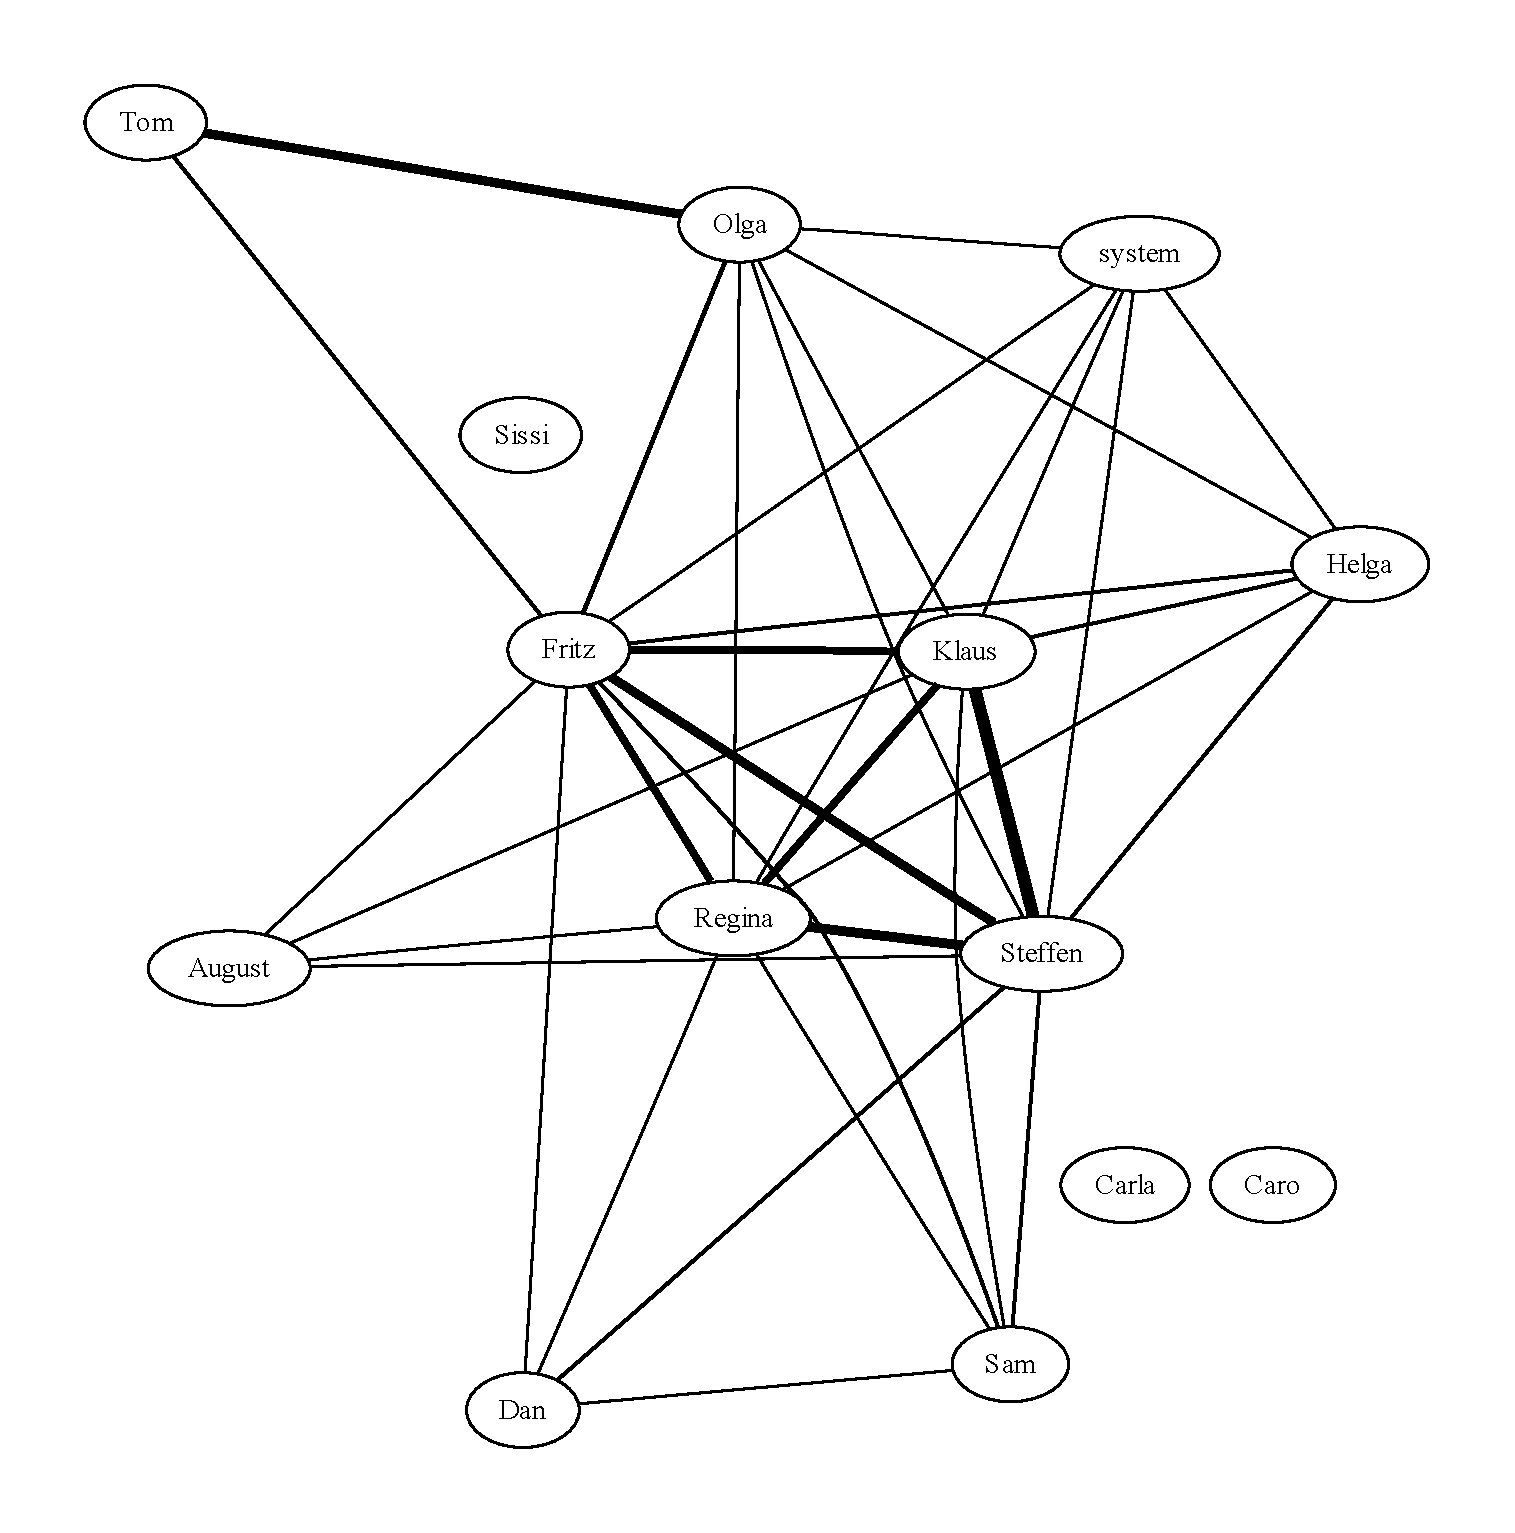
\includegraphics[width=.5\linewidth]{gv_ca-noweights}\hfill
  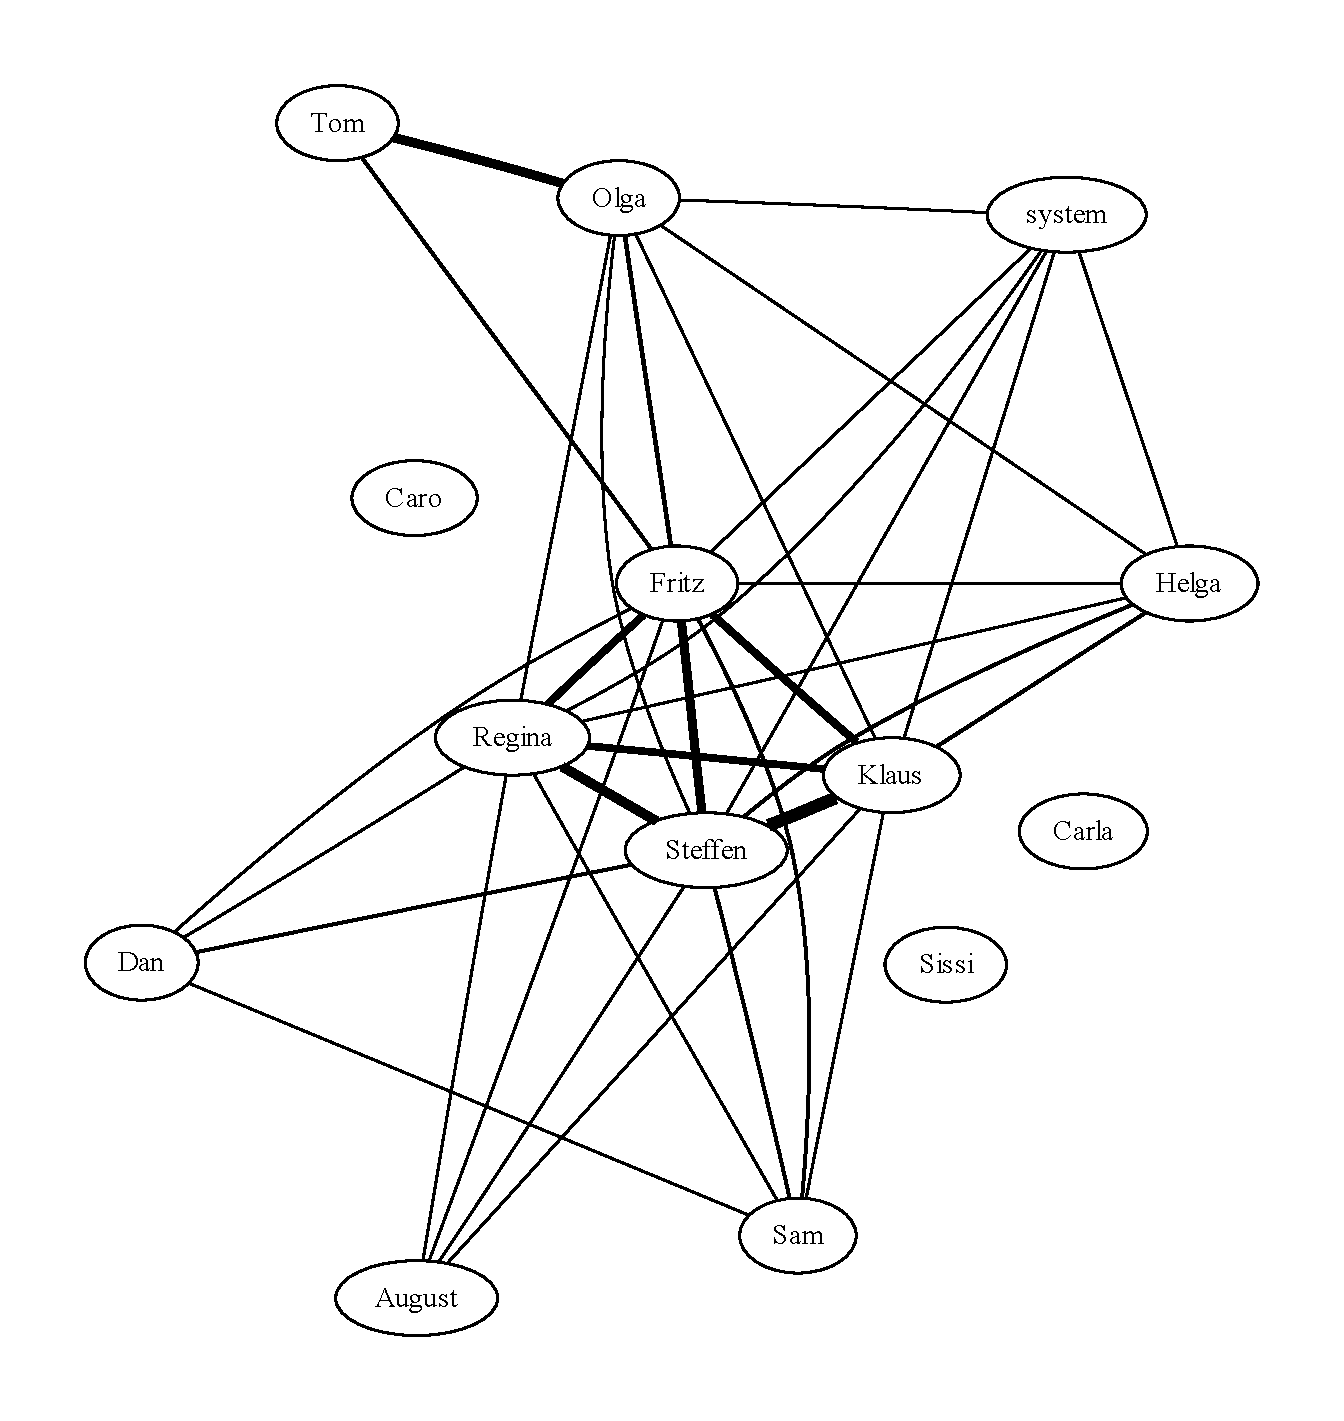
\includegraphics[width=.45\linewidth]{gv_ca-weights}
  \caption{coauthorgraphs without and with edge weights used for
    layout}
  \label{fig:gv_ca-weights}
\end{figure}

As we could see in figures~\ref{fig:gv-catwopi5}
and~\ref{fig:gv-catcirco} graphs are by default created with weighted
edges. We can use these edge weights in different ways. Some of the
graphviz layout engines can use weight information to compute node
positions:
\begin{typed}
\p{irb(main):034:0>} \c{cgraph = wiki.coauthorgraph; nil}
=> nil
\p{irb(main):117:0>} \c{cgraph.to_graphviz('gv_ca-noweights.pdf', 'neato', :pdf,
                     'overlap=false', 'splines=true') \{ |weight| 
\hfill ["penwidth=#\{weight**0.5\}", "len=4"] \}}
=> #<IO:0xf655be7c>
\p{irb(main):118:0>} \c{cgraph.to_graphviz('gv_ca-weights.pdf', 'neato', :pdf,
                     'overlap=false', 'splines=true') \{ |weight| 
\hfill ["penwidth=#\{weight**0.5\}", "len=#\{4/weight**0.25\}"] \}}
=> #<IO:0xf654cb20>
\end{typed}
The \code{neato} layout engine takes ``\code{len}'' as an edge
attribute and tries to lay out the nodes in a way that all edges are
close to these lengths. We used this here to drag intense coauthors
close together, as you can see in figure~\ref{fig:gv_ca-weights} (right).
Additionally we exposed the edge weights by changing the pen
width. We could have accomplished a similar effect by changing the
edge color from grey to black using the weight.

\subsection{Graph Generation Methods}
\label{sec:graphmethods}

\begin{figure}
  \centering
  \parbox[b]{.33\textwidth}{\vspace{-5ex}
  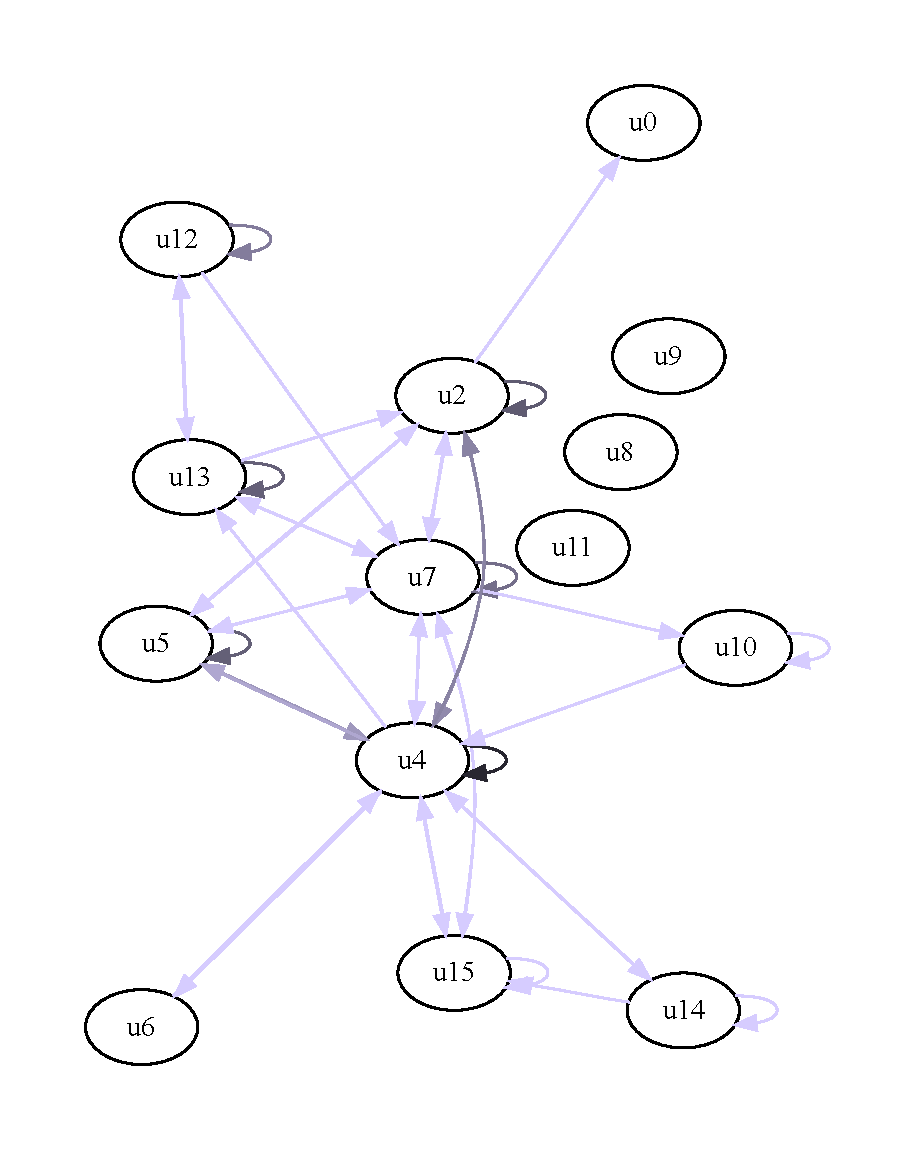
\includegraphics[width=\linewidth]{gv_drg}\vspace{-5ex}
  \caption{directresponse}
  \label{fig:gv_drg}}\hfill
  \parbox[b]{.33\textwidth}{
  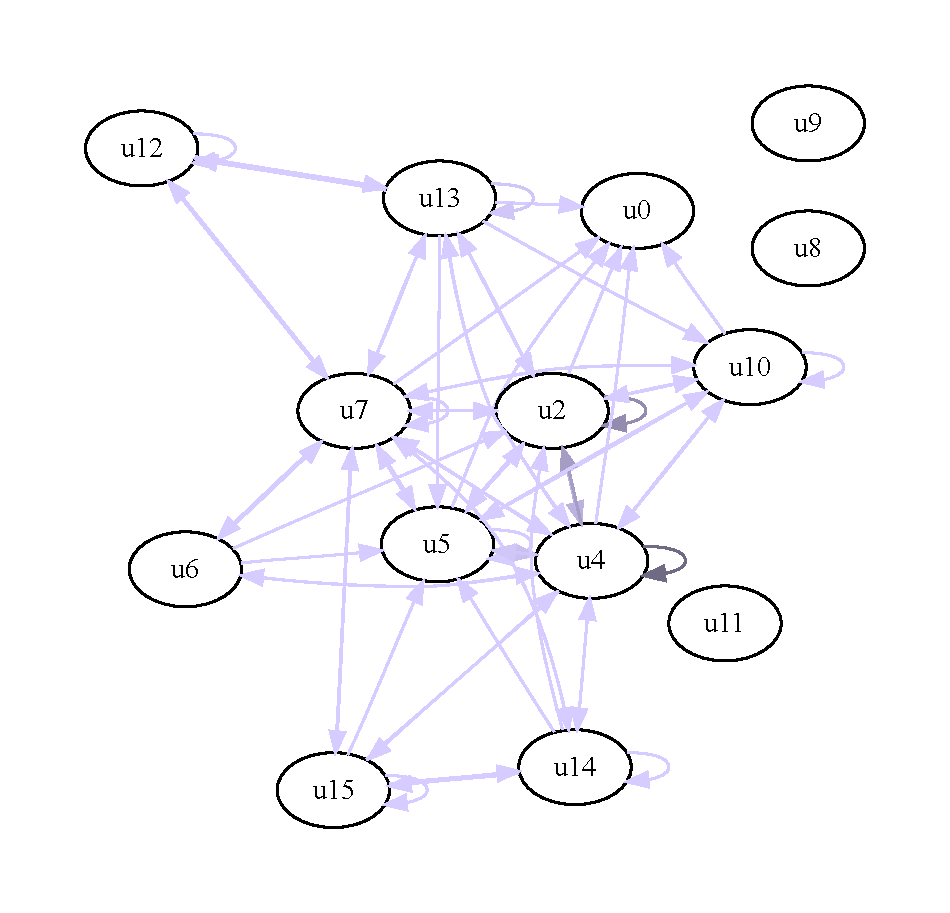
\includegraphics[width=\linewidth]{gv_grg}\vspace{-3ex}
  \caption{groupresponse}
  \label{fig:gv_grg}}\hfill
  \parbox[b]{.33\textwidth}{
  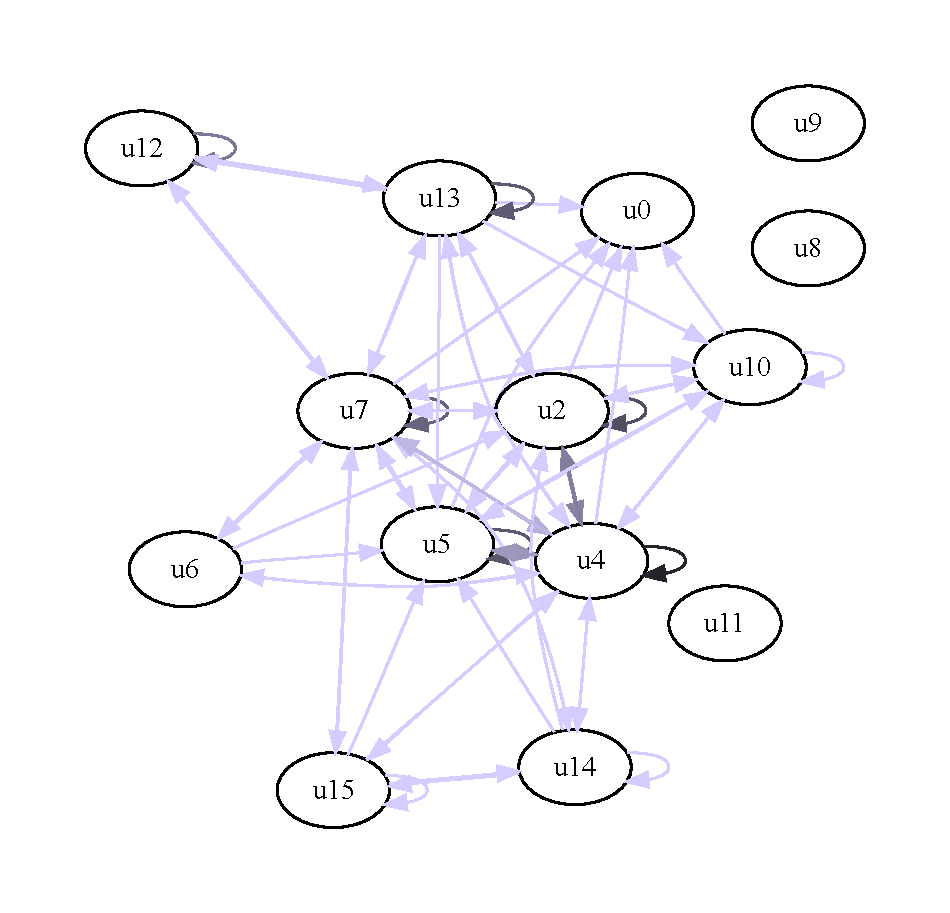
\includegraphics[width=\linewidth]{gv_ilrg}\vspace{-3ex}
  \caption{interlocking}
  \label{fig:gv_ilrg}}
\end{figure}

You may have noticed by reading \rdoc{Mediawiki::Wiki.coauthorgraph}
in the method documentation that the edge weights can be computed in
two different ways. By default coauthorship edges are weighted by the
number of pages two users share, but you may prefer the Newman measure
(see \cite{Newman:2001zr,Newman:2001mz}).

The copagesgraph connects users by the pages they edit but does not
use the linear structure of the page history for more detailed
measures. You may interpret the edit history of a page as a kind of
dialogue between users: each edit is an answer to the edit
before. This is done by the
\rdoc{Mediawiki::Wiki.directresponsegraph}.  It gives a rather sparse
graph with directed edges, as two users are only connected if they
have successive edits on a page.  Alternatively we can use
\rdoc{Mediawiki::Wiki.groupresponsegraph}. Here an edit is considered
as answer to all precedent edits, which gives a directed graph similar
to the coauthorgraph.

The direct response graph is too picky and the group response graph
is too coarse and both do not reflect the page history structure very
well. So we developed the interlocking response graph which lays kind of
in between (see \cite{Stein/Blaschke:2009a,Blaschke/Stein:2007} for a
detailed discussion).

\begin{typed}
\p{irb(main):241:0>} \c{wiki.directresponsegraph \{ |n| n.uid \}.to_graphviz('gv_drg.pdf', 
                                'neato', 'pdf', 'overlap=false', 'splines=true',
                                'edge [len=2]') \{ |w| 
\hfill ["color=\textbackslash"0.7 0.2 #\{4/w**0.5\}\textbackslash""] \}}
=> #<IO:0xf65fcc3c>
\p{irb(main):242:0>} \c{wiki.groupresponsegraph \{ |n| n.uid \}.to_graphviz('gv_grg.pdf', 
                                'neato', 'pdf', 'overlap=false', 'splines=true',
                                'edge [len=2]') \{ |w|
\hfill ["color=\textbackslash"0.7 0.2 #\{4/w**0.5\}\textbackslash""] \}}
=> #<IO:0xf655f52c>
\p{irb(main):245:0>} \c{wiki.interlockingresponsegraph \{ |n| n.uid \}.to_graphviz(
                 'gv_ilrg.pdf', 'neato', 'pdf', 'overlap=false', 'splines=true',
                                'edge [len=2]') \{ |w|
\hfill ["color=\textbackslash"0.7 0.2 #\{4/w**0.5\}\textbackslash""] \}}
=> #<IO:0xf64e0074>
\end{typed}
Group response and interlocking have the same links but different link
weights.\footnote{You may have to adapt color computation for your
  wiki. To get best results we could have asked the graph for the
  maximum link weight.}

All three methods take various parameters to finetune how exactly the
link weights are computed (see the given citations for a discussion of
these). interlocking can also be used to create animations using
\rdoc{Mediawiki::Wiki.timedinterlockingresponsegraph}. We will discuss
this in section~\ref{sec:sonia}.

The group response graph and the interlocking graph visually do not
differ much from the coauthorship graph. Their strength lies in the
statistical measures as the following example shows:
\begin{typed}
\p{irb(main):256:0>} \c{wiki.interlockingresponsegraph(:counts => :max).
\hfill pp_degrees(:counts => true, :sortby => 1)}
Node                          :  deg  out   in
Steffen                       :  145   71   74
Regina                        :   84   40   44
Fritz                         :   73   38   35
Klaus                         :   66   33   33
Olga                          :   48   25   23
Tom                           :   39   20   19
Sam                           :   22   13    9
Dan                           :   17    9    8
Helga                         :   16    8    8
...
=> nil
\p{irb(main):257:0>} \c{wiki.interlockingresponsegraph(:counts => :page).
\hfill pp_degrees(:counts => true, :sortby => 1)}
Node                          :  deg  out   in
Steffen                       :  241  123  118
Klaus                         :  156   74   82
Fritz                         :  111   56   55
Regina                        :  100   49   51
Olga                          :   71   41   30
Tom                           :   54   24   30
Helga                         :   15    6    9
Sam                           :   14    9    5
Dan                           :   10    6    4
...
=> nil
\end{typed}
While Regina has a higher collaborative depth Klaus wins for
collaborative breadth (ok, Steffen outperforms all others). 

\bigskip

The reverse concept to coauthorship is the copages graph. While the
former connects authors by pages the latter connects pages by authors,
i.\,e., two pages are linked if they have at least one common author. 

We now have two page graphs: the hyperlink pagegraph showing which
pages are explicitly linked by the users and the copages graph
connecting pages which have at least one common author:

\begin{figure}
  \parbox[b]{.6\textwidth}{
  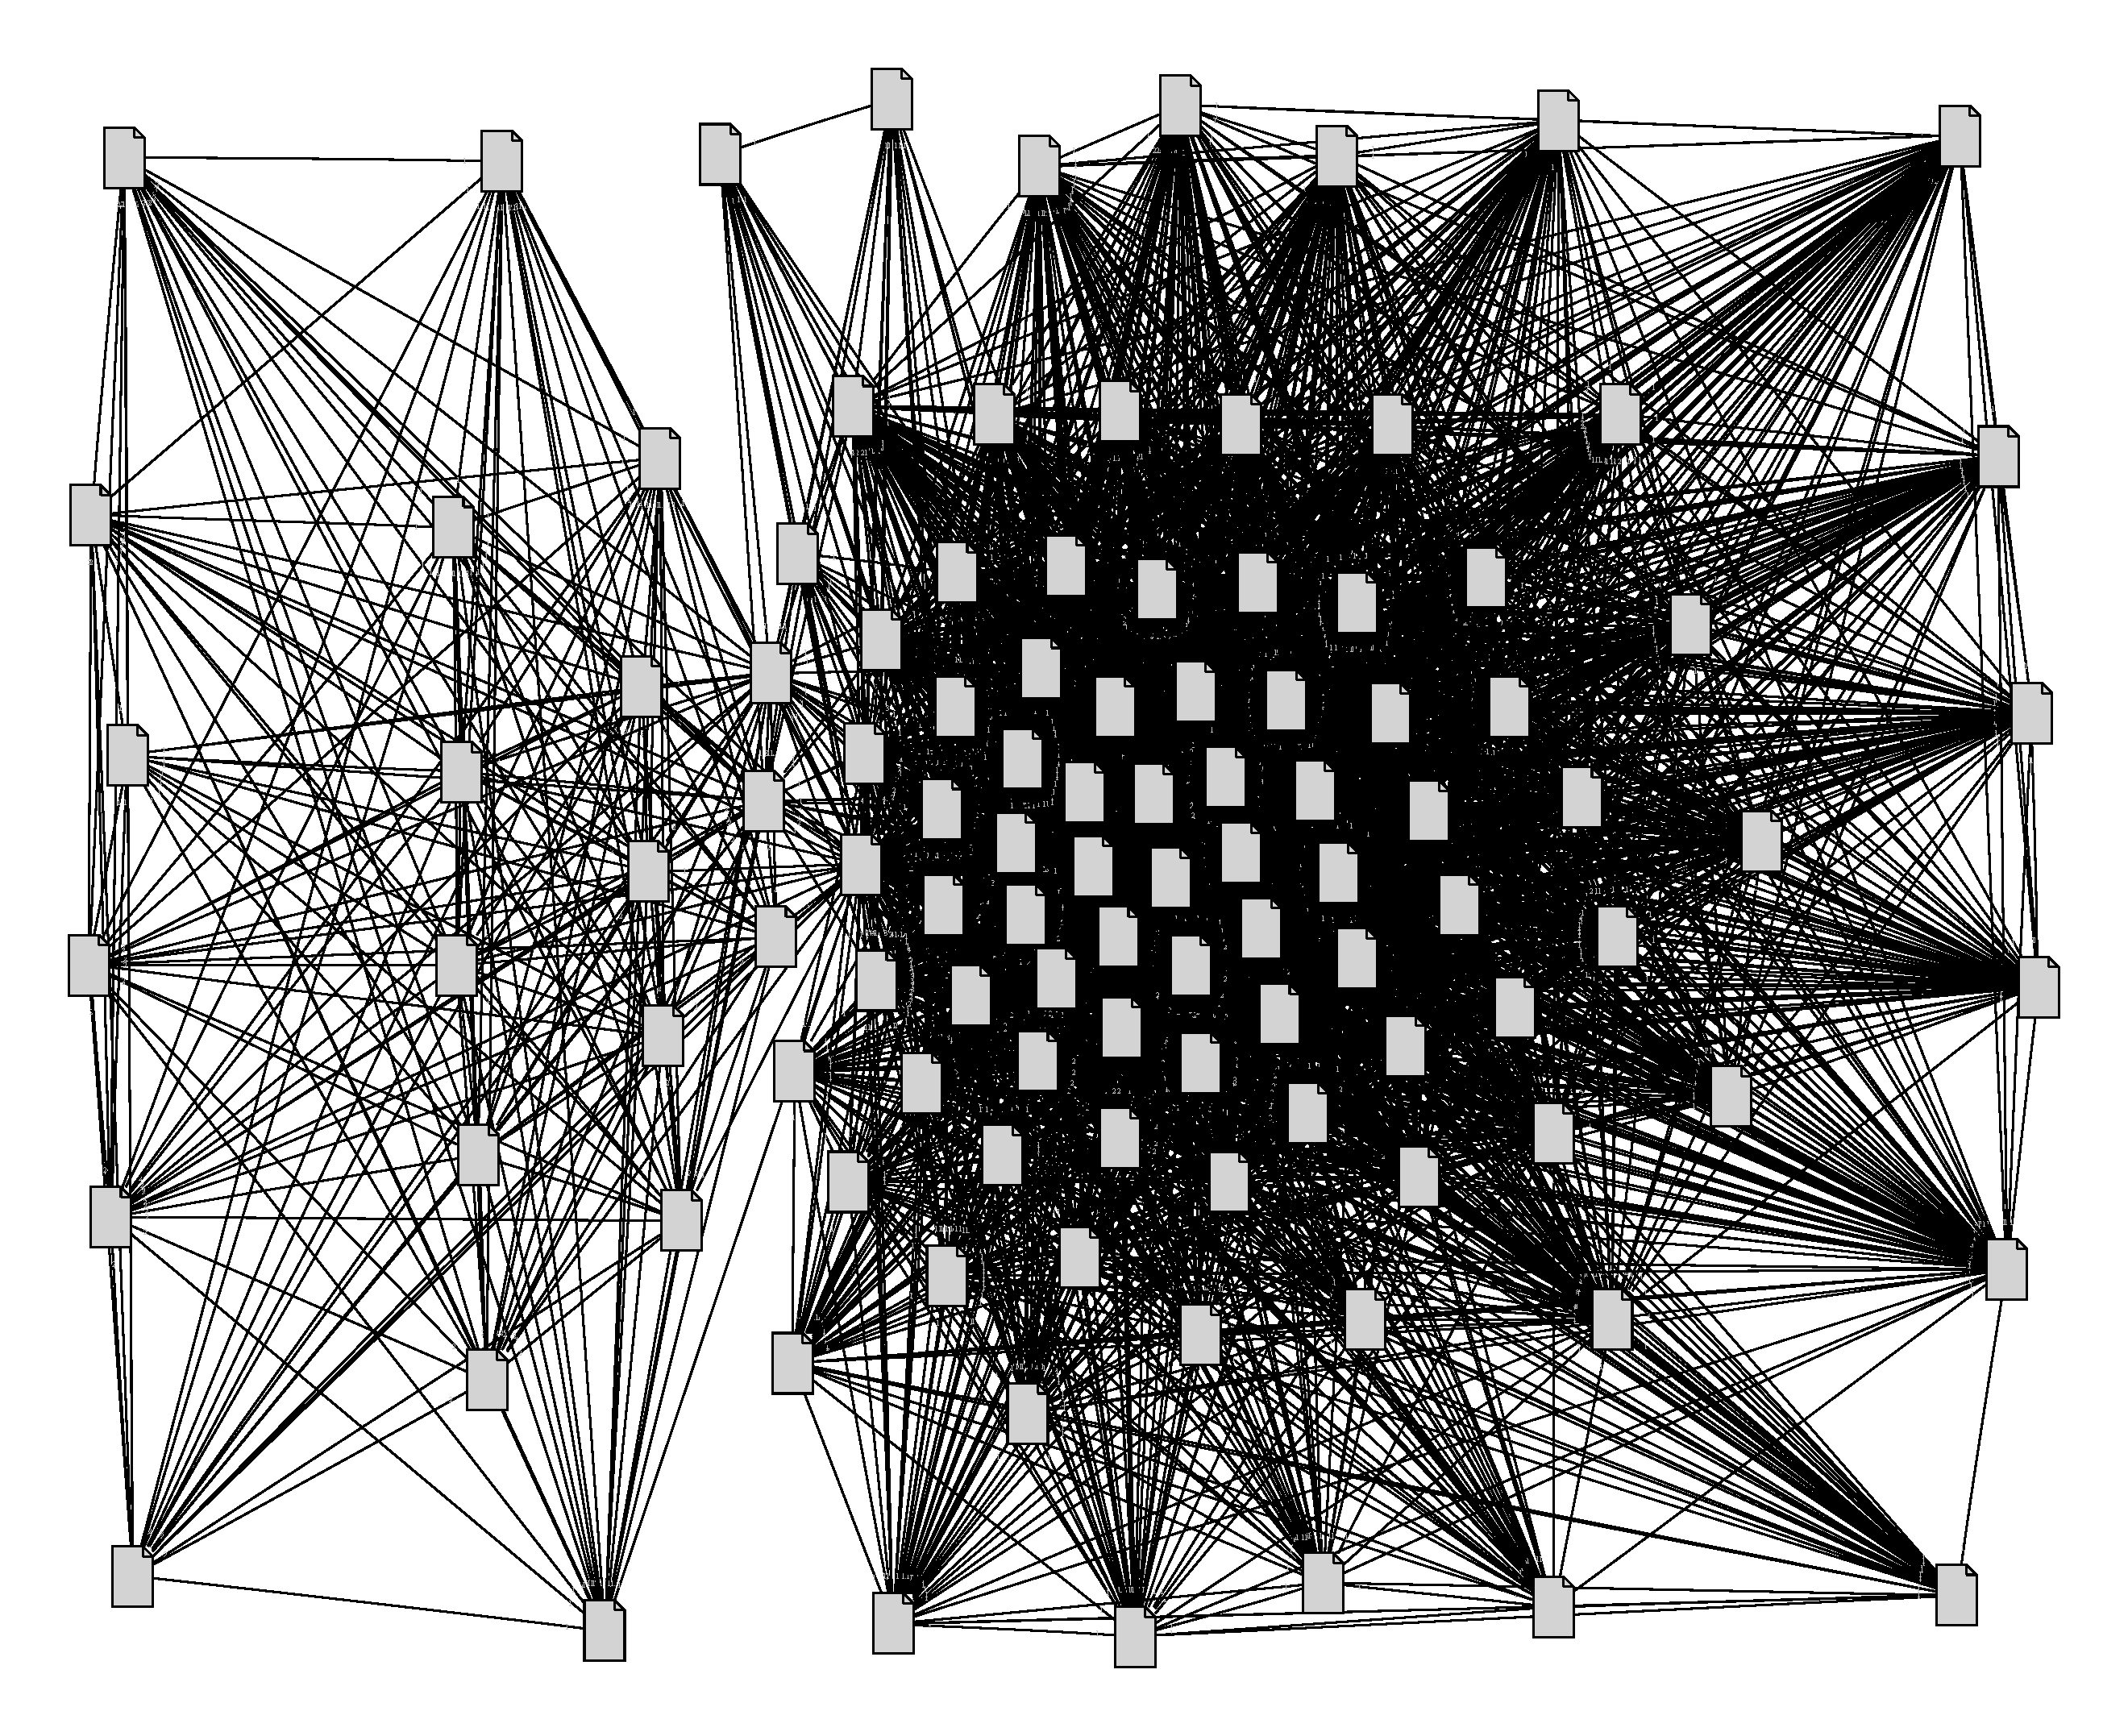
\includegraphics[width=\linewidth]{copages}\vspace{-2ex}
  \caption{copages graph}
  \label{fig:copages}}%
\parbox[b]{.4\textwidth}{
  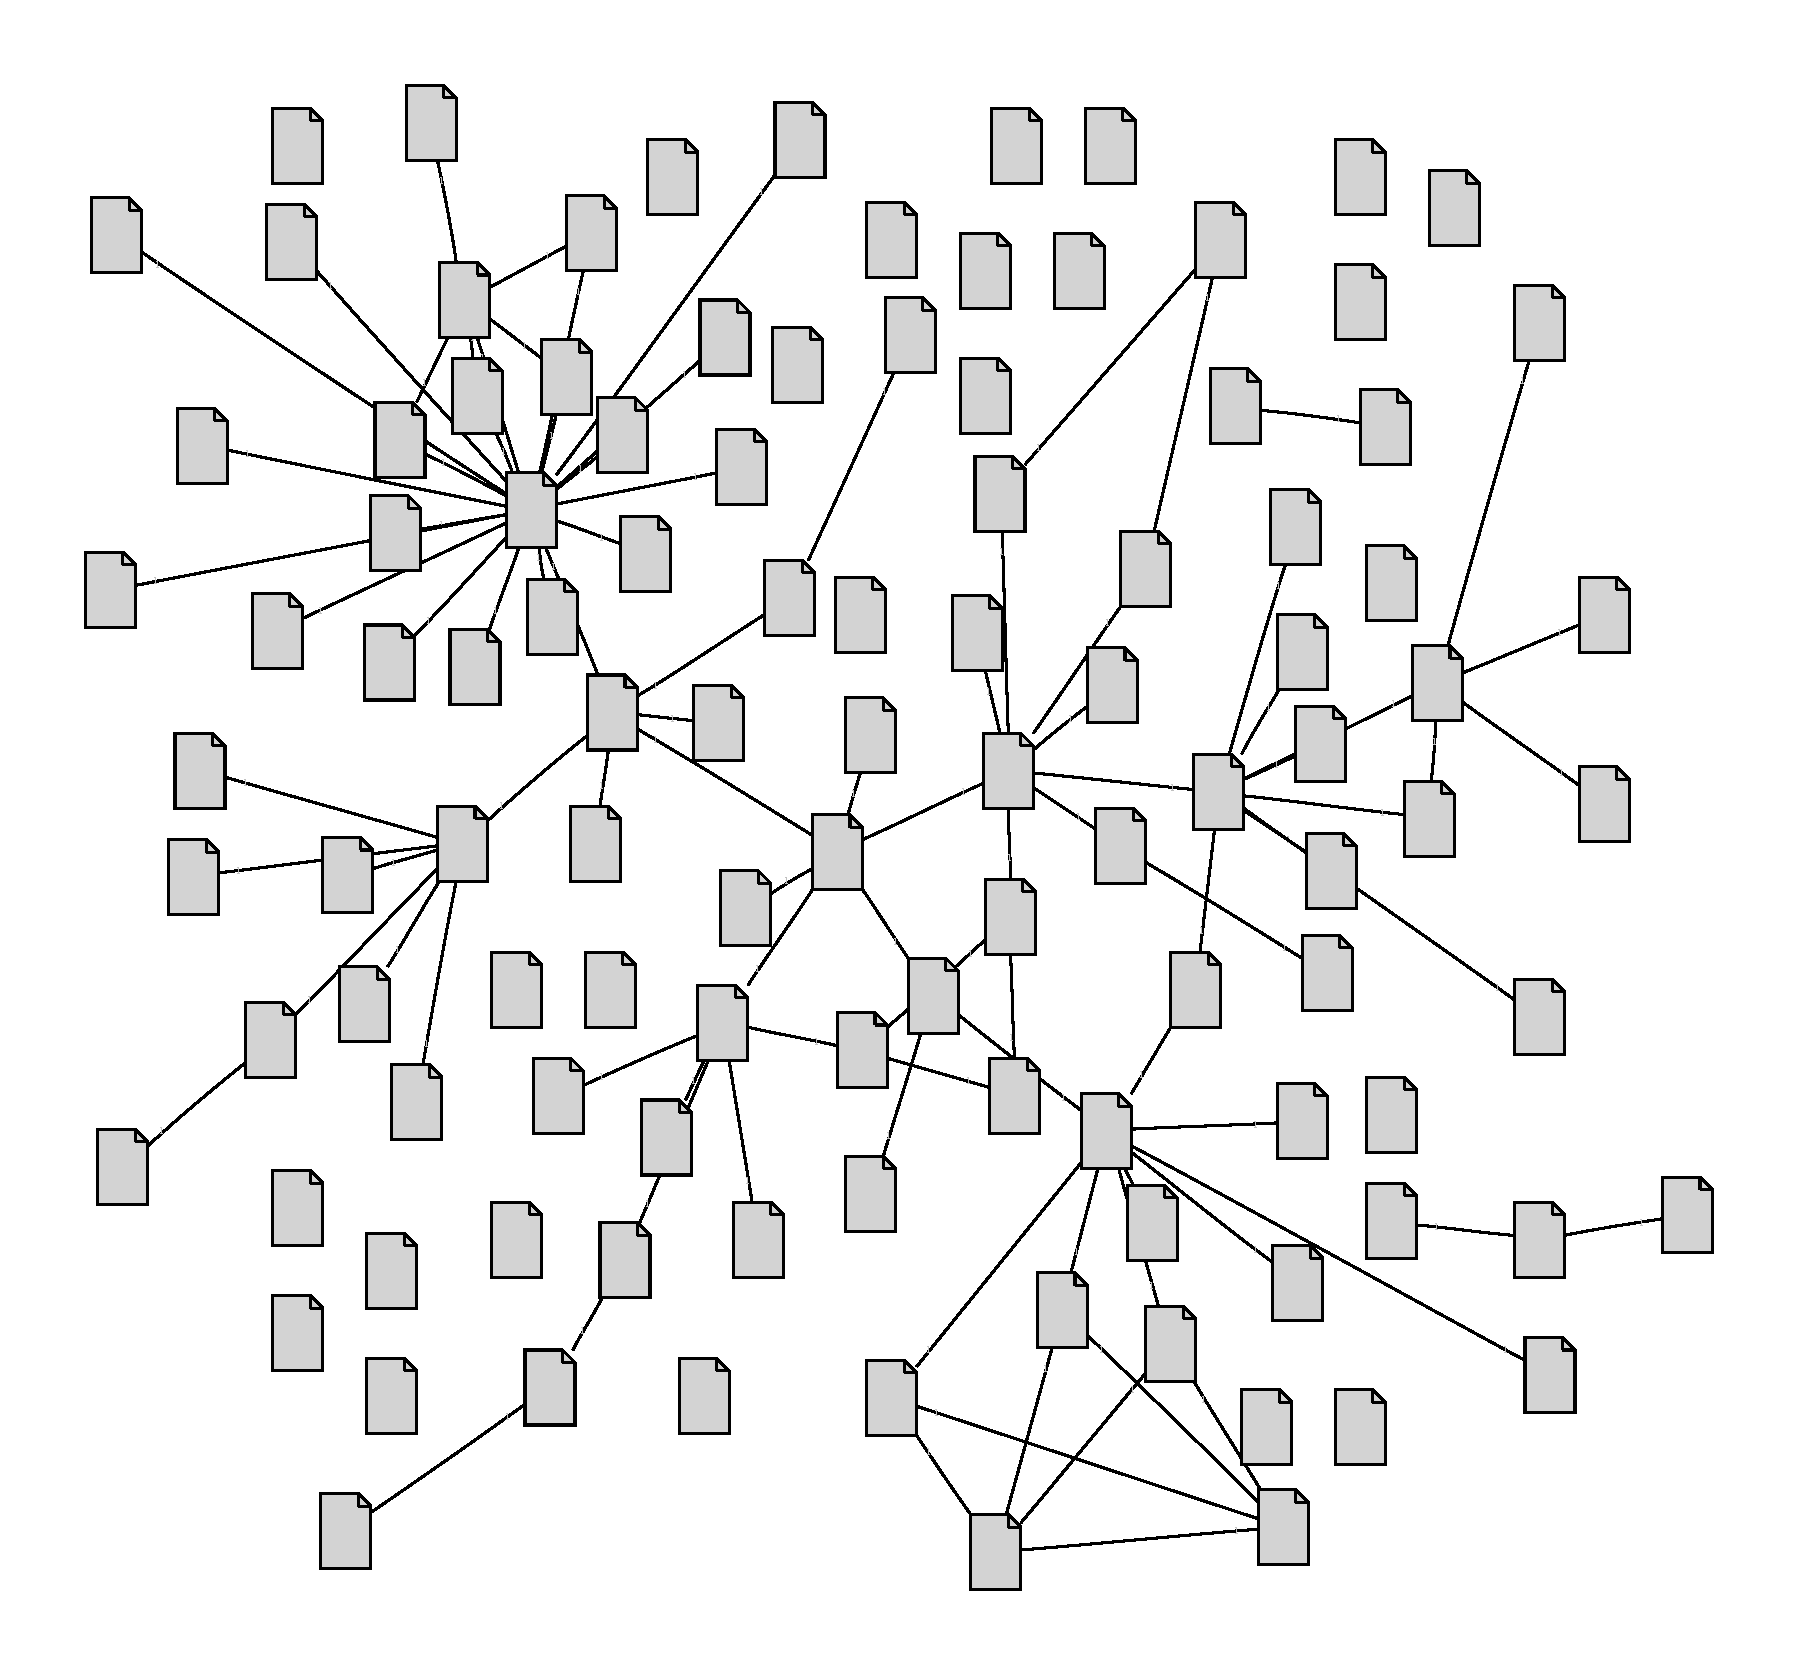
\includegraphics[width=\linewidth]{pg-copg}\vspace{4ex}
  \caption{links$-$copages}
  \label{fig:copages}}
\end{figure}

\begin{typed}
\p{irb(main):064:0>} \c{wiki.copagesgraph \{''\}.to_graphviz('copages.pdf', :neato, :pdf, 
                                   'outputorder=edgesfirst', 'overlap=false', 
                                   'node [shape=note, style=filled, width=.34]')}
=> #<IO:0xf6701ad8>
\end{typed}
We see that while most pages are well connected there is kind of a
cluster to the left with only little connection to the rest. We could
add node labels or create an SVG with tooltips to see which pages do
the connection. Let's go one step further:
\begin{typed}
\p{irb(main):111:0>} \c{pg = wiki.pagegraph; nil}
=> nil
\p{irb(main):112:0>} \c{copg = wiki.copagesgraph; nil}
=> nil
\p{irb(main):113:0>} \c{pg_copg = DotGraph.new(pg.nodes) \{''\}; nil}
=> nil
\p{irb(main):114:0>} \c{pg.links.each \{ |a,l| pg_copg.link(*a) unless copg.links[a] \}; 
\hfill nil}
=> nil
\p{irb(main):115:0>} \c{pg_copg.to_graphviz('pg-copg.pdf', :neato, :pdf, 
                                   'outputorder=edgesfirst', 'overlap=false', 
                                   'node [shape=note, style=filled, width=.34]')}
=> #<IO:0xf66f2754>
\end{typed}
Here we created a \emph{new} graph with pages as nodes and set an edge
between two nodes if they are connected in the page graph and not
connected in the copages graph (we kind of substract the copages from
the page graph). This gives us the pages which are explicitly linked
in the wiki but are edited by different groups of users.

\subsection{Edge Weight Filters}
\label{sec:edgefilter}

\begin{figure}
  \begin{tabular}{@{}c@{}c@{}c@{}c@{}}
    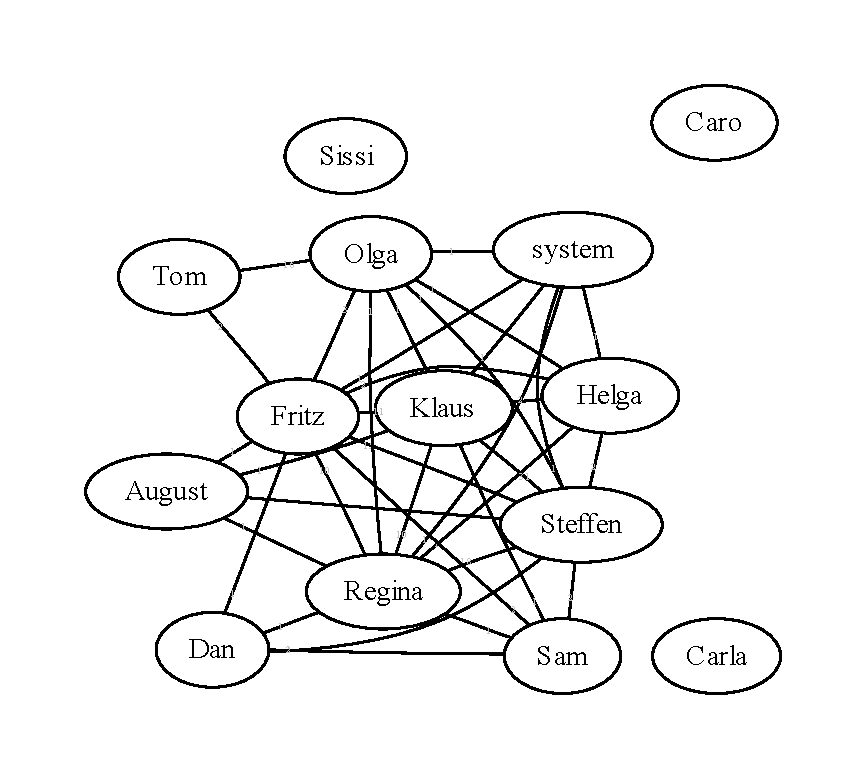
\includegraphics[width=.25\linewidth]{gv_ca0} &
    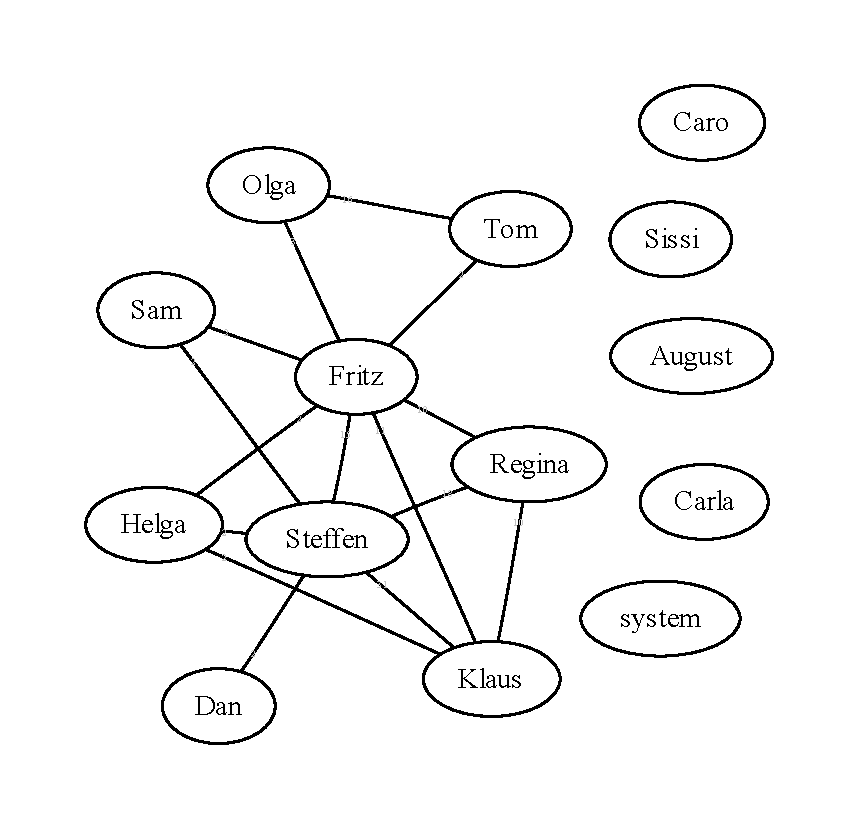
\includegraphics[width=.25\linewidth]{gv_ca1} &
    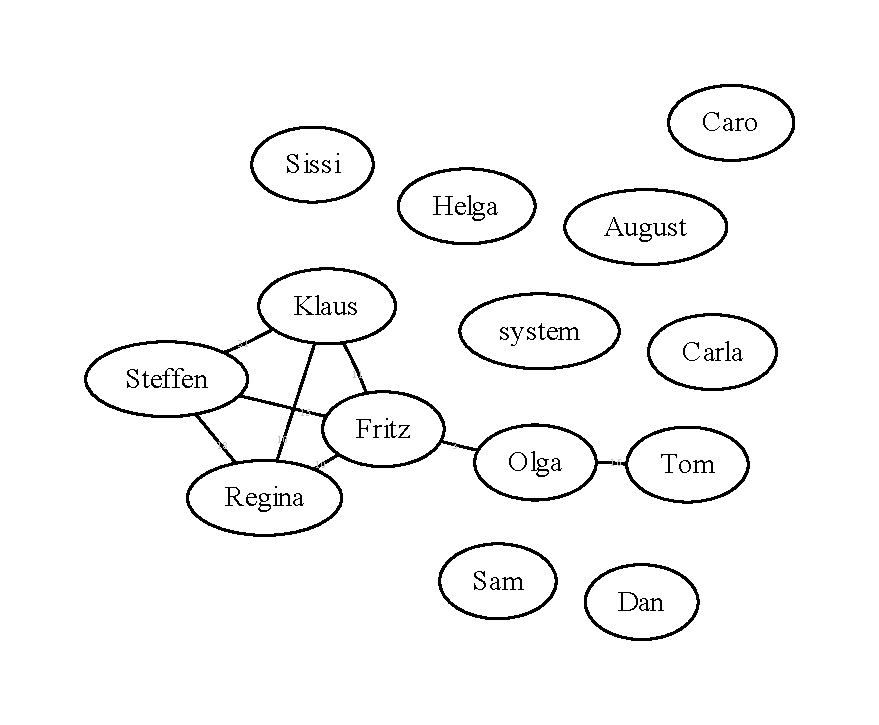
\includegraphics[width=.25\linewidth]{gv_ca2} & 
    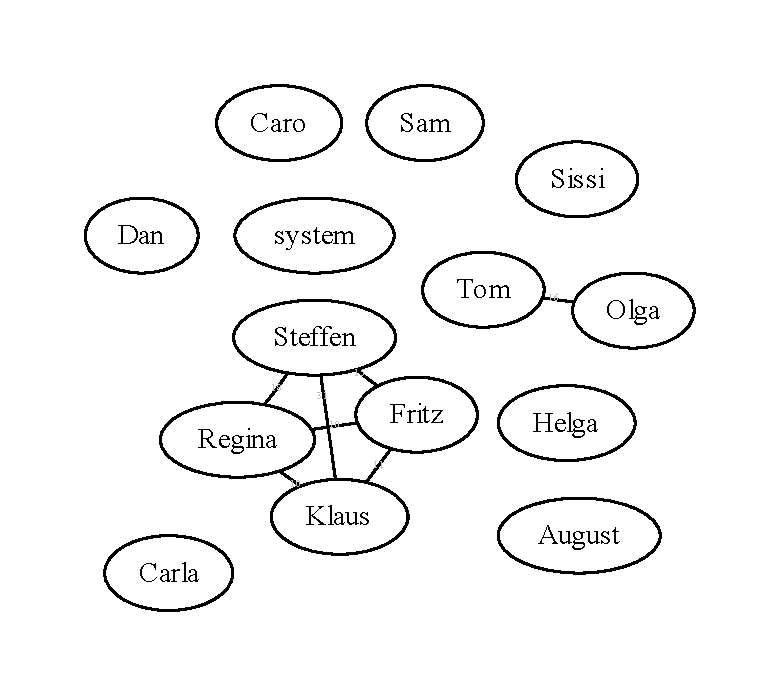
\includegraphics[width=.25\linewidth]{gv_ca3}\\
    full & $w>1$ & $w>2$ & $w>3$
  \end{tabular}
  \caption{edge weight filtered coauthor graph}
  \label{fig:ca-weightfilter}
\end{figure}

We learned before how to use edge weights for graph layout. One way to
visualize connection strength is edge filtering: we remove all edges
below a certain weight and show the remaining graph
(figure~\ref{fig:ca-weightfilter}):
\begin{typed}
\p{irb(main):264:0>} \c{cgraph = wiki.coauthorgraph; nil}
\p{irb(main):265:0>} \c{params = ['neato', :pdf, 'overlap=false', 'splines=true']}
\p{irb(main):266:0>} \c{cgraph.to_graphviz('gv_ca0.pdf', *params)}
=> #<IO:0xf6518528>
\p{irb(main):267:0>} \c{cgraph.remove_links(1.1); nil}
=> nil
\p{irb(main):268:0>} \c{cgraph.to_graphviz('gv_ca1.pdf', *params)}
=> #<IO:0xf650ddf8>
\p{irb(main):269:0>} \c{cgraph.remove_links(2.1); nil}
=> nil
\p{irb(main):270:0>} \c{cgraph.to_graphviz('gv_ca2.pdf', *params)}
=> #<IO:0xf6503678>
\p{irb(main):271:0>} \c{cgraph.remove_links(3.1); nil}
=> nil
\p{irb(main):272:0>} \c{cgraph.to_graphviz('gv_ca3.pdf', *params)}
=> #<IO:0xf64f9808>
\end{typed}
You get a clear picture about who is working together, and you cannot
only print these graphs, you can also apply network measures on them
etc. (did you like my nice trick with the additional \cmd{params} variable?)

The only drawback may be that the nodes change their position from one
step to the other, as the layout manager renders the network with less
edges different. So what I would like to do is to render the graph
once (with all edges), fix the node positions and remove some edges
and render it again. And we can do this by computing node positions
once and using them for all four graphs as the following example will
show, now featuring the interlocking response graph:\footnote{please
  note that \cmd{render\_graphviz} may trigger a graphviz bug if you
  decided to use \file{dotgraph-gv} and your graphviz version is older
than 2009-8-7.}

\begin{figure}
  \centering
  
  \begin{tabular}{@{}c@{}c@{}c@{}c@{}}
    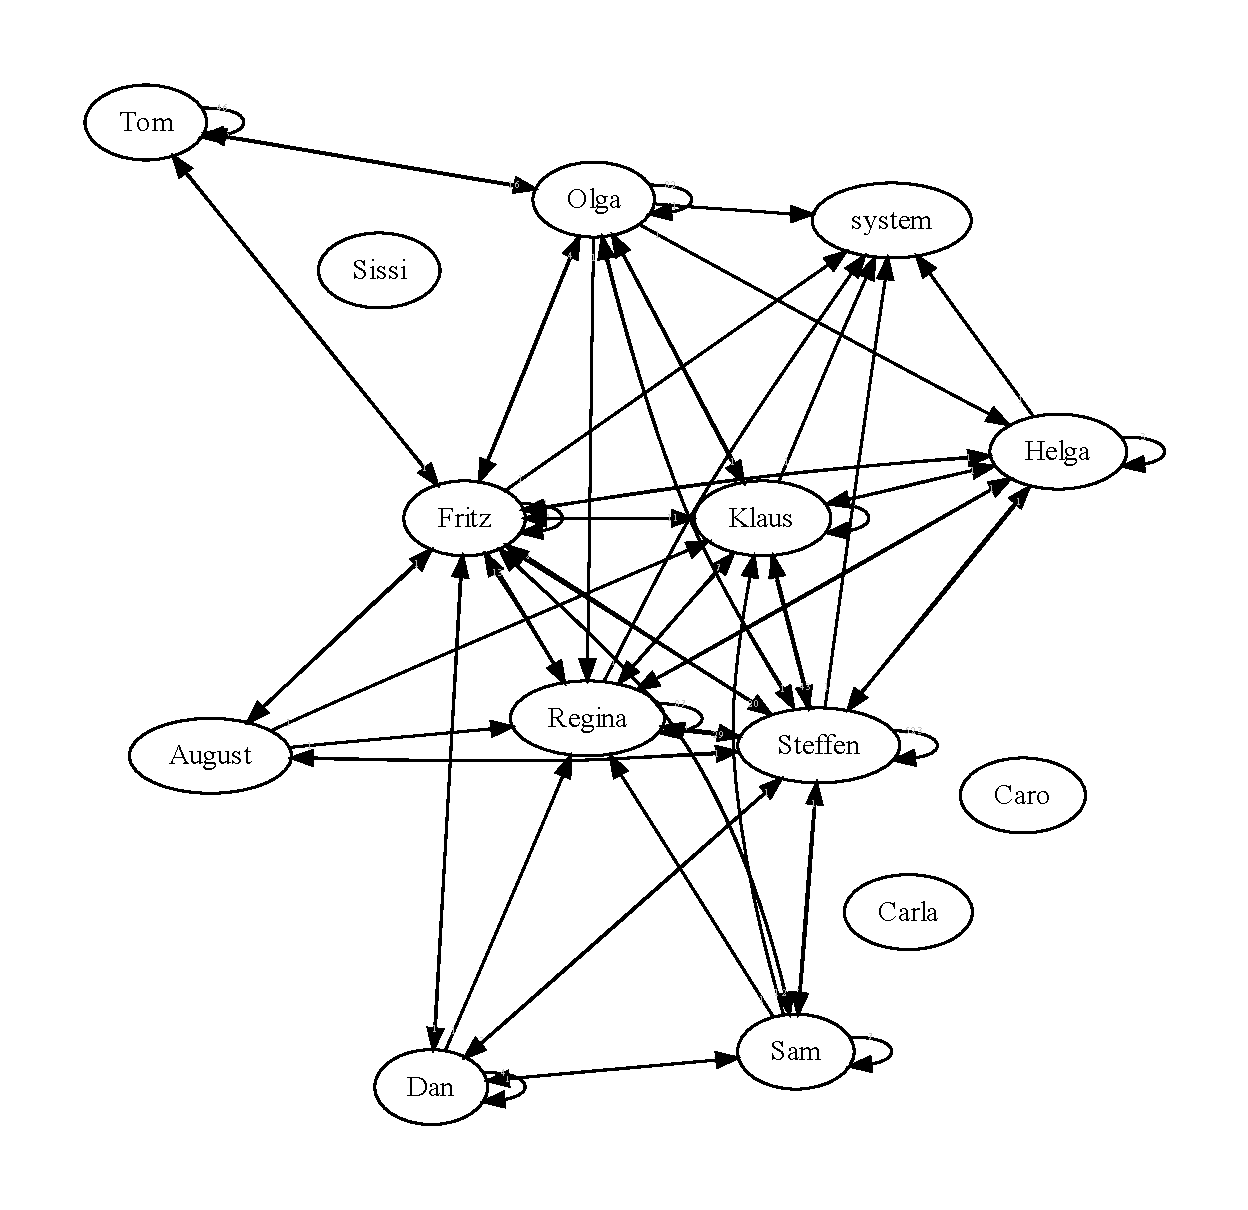
\includegraphics[width=.25\linewidth]{gv_il0} &
    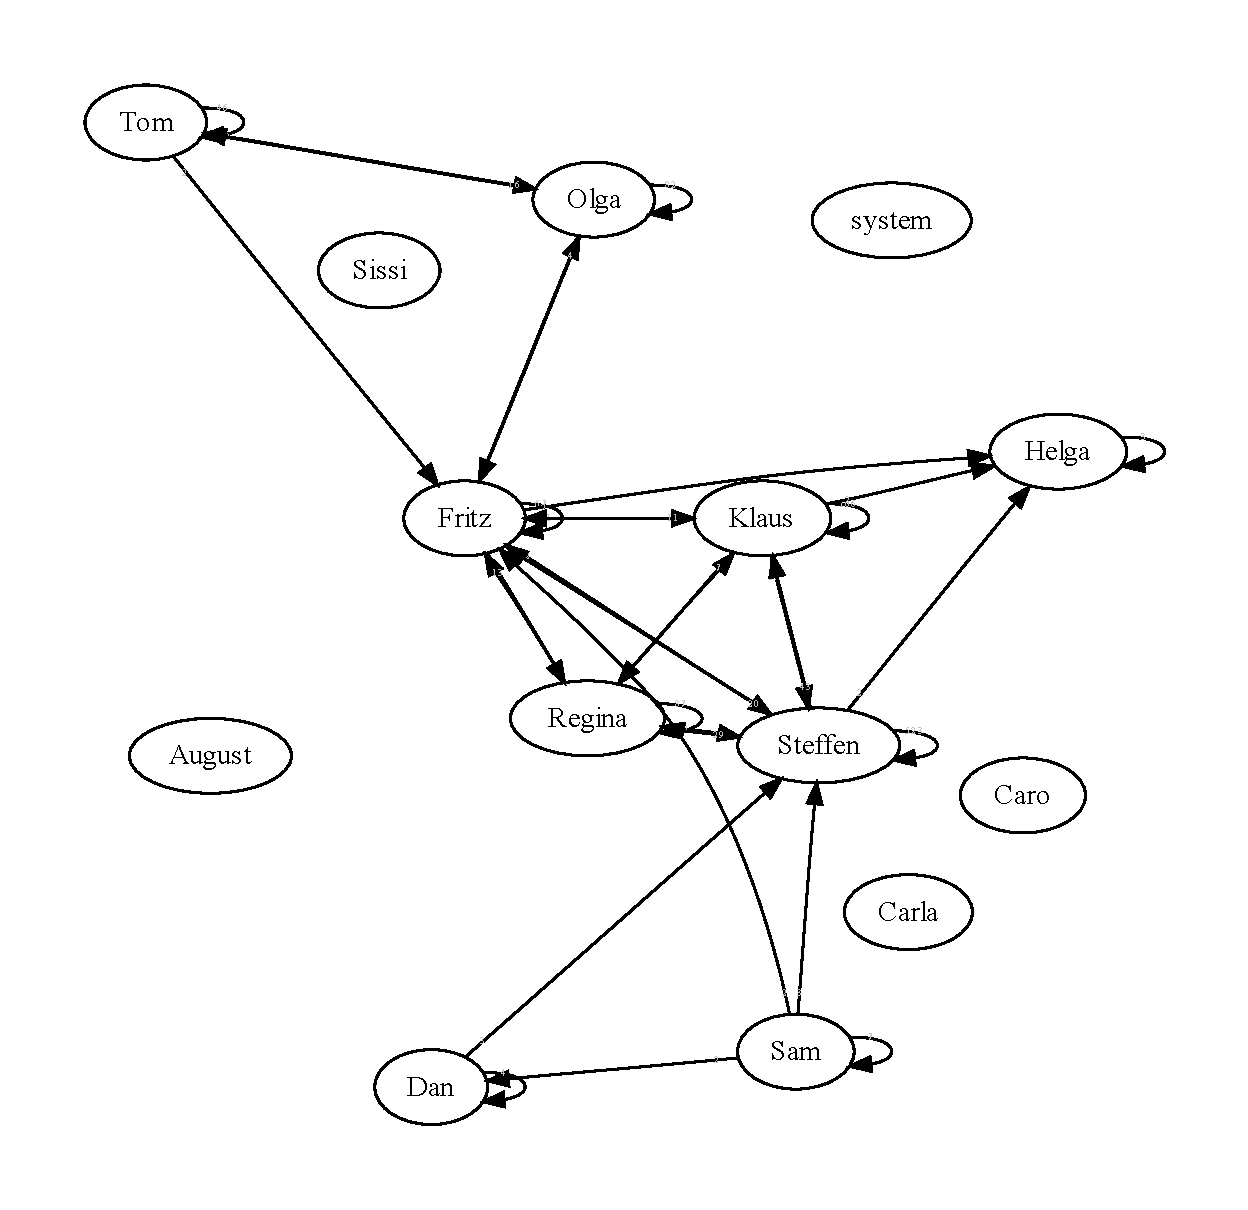
\includegraphics[width=.25\linewidth]{gv_il1} &
    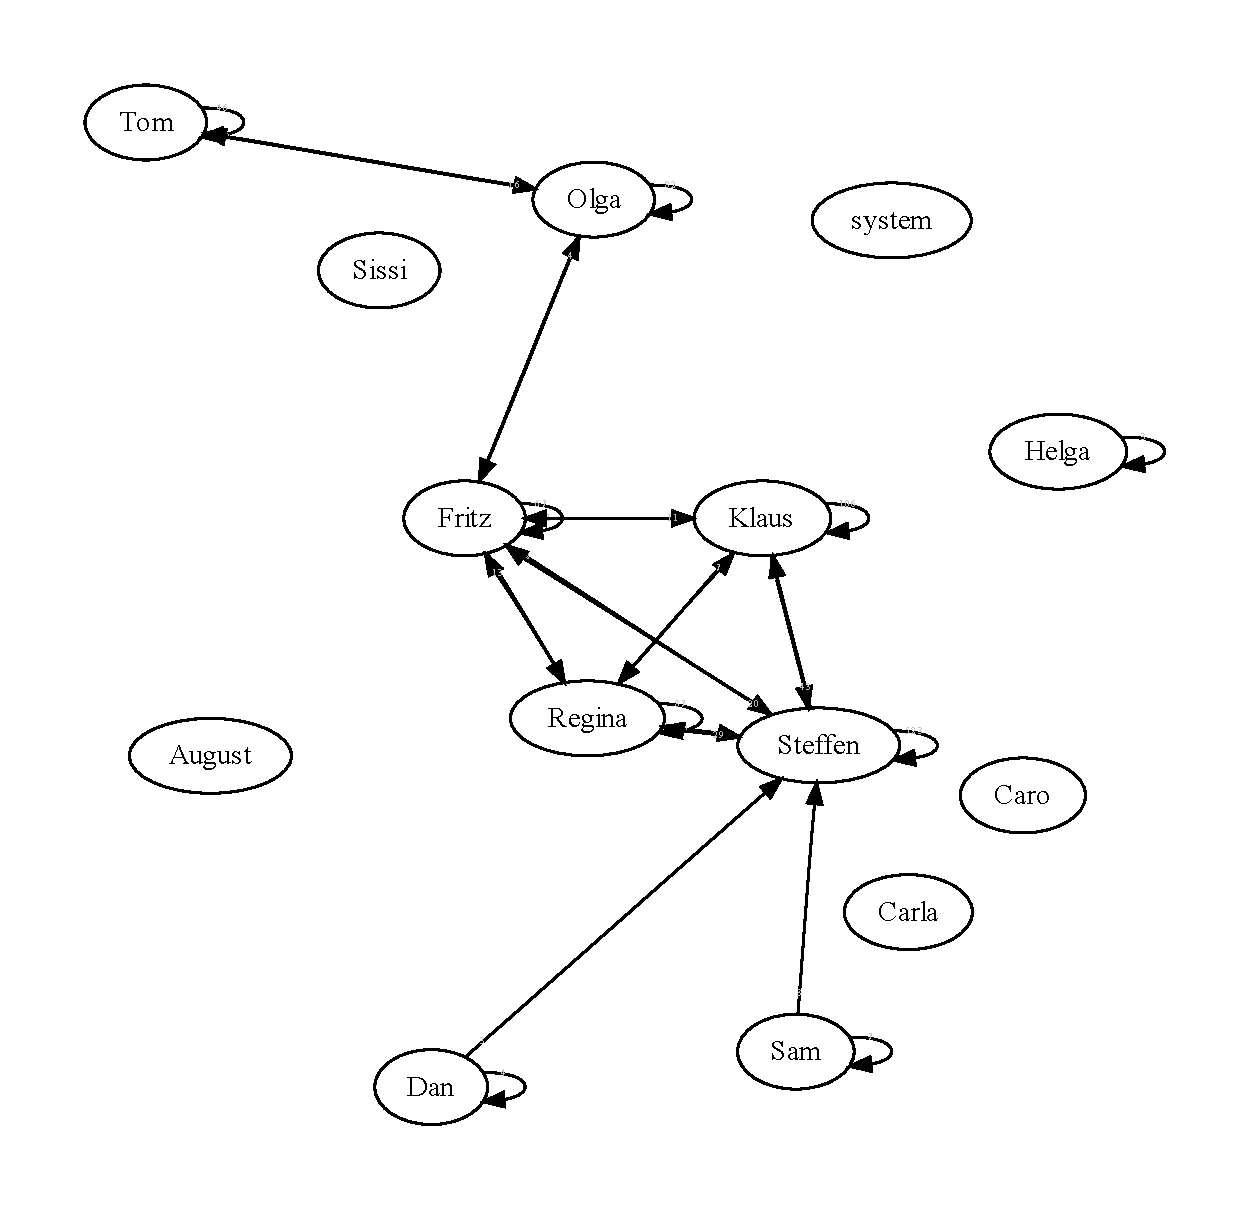
\includegraphics[width=.25\linewidth]{gv_il2} & 
    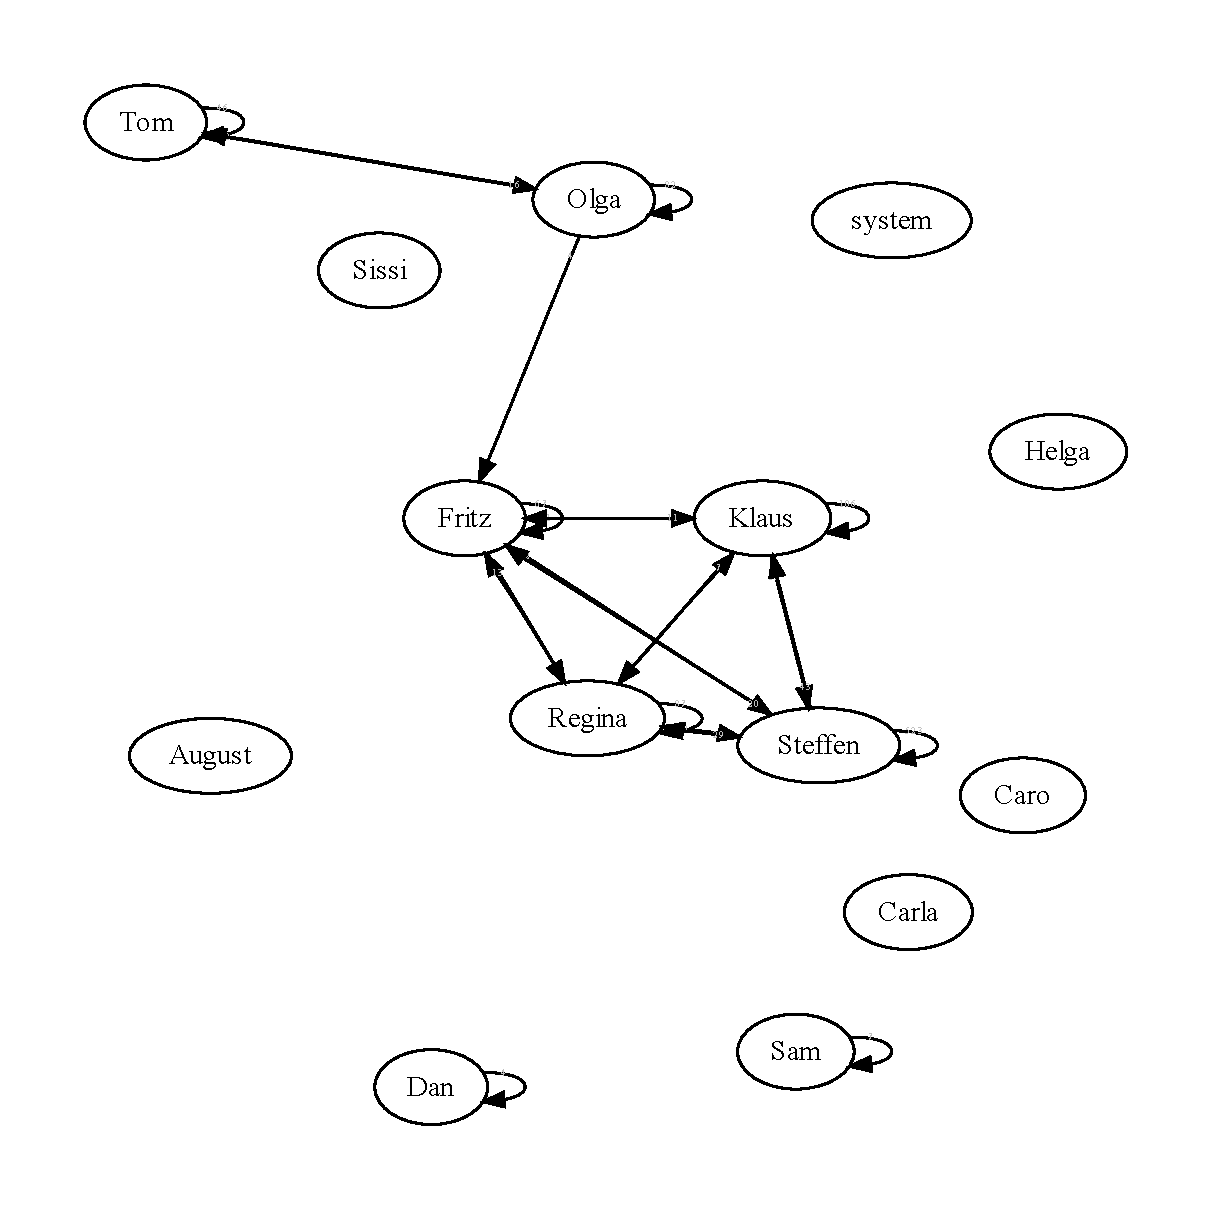
\includegraphics[width=.25\linewidth]{gv_il3}\\
    full & $w>1$ & $w>2$ & $w>3$
  \end{tabular}
  \caption{edge weight filtered interlocking graph with fixed node positions}
  \label{fig:il-weightfilter}
\end{figure}

\begin{typed}
\p{irb(main):014:0>} \c{ilgraph = wiki.interlockingresponsegraph; nil}
=> nil
\p{irb(main):015:0>} \c{gparams = ['overlap=scale', 'splines=true', 'edge [len=3]']}
=> ["overlap=scale", "splines=true", "edge [len=3]"]
\p{irb(main):016:0>} \c{nodepos = ilgraph.render_graphviz(:neato, *gparams)}
=> \{"u12"=>"30,482", "u5"=>"242,196", "u13"=>"245,445", "u6"=>"61,178", ...\}
\p{irb(main):017:0>} \c{ilgraph.nodeblock \{ |n| ["label=\textbackslash"#\{n.name\}\textbackslash"", 
                                          "pos=\textbackslash"#\{nodepos[ilgraph.nid(n)]\}\textbackslash"", 
                                          'pin'] \}}
=> #<Proc:0xf6699474@(irb):17>
\p{irb(main):018:0>} \c{ilgraph.to_graphviz('gv_il0.pdf', :nop, 'pdf', *gparams)}
=> #<IO:0xf6694398>
\p{irb(main):021:0>} \c{ilgraph.remove_links(1.1); nil}
=> nil
\p{irb(main):022:0>} \c{ilgraph.to_graphviz('gv_il1.pdf', :nop, 'pdf', *gparams)}
=> #<IO:0xf6662de8>
\p{irb(main):023:0>} \c{ilgraph.remove_links(2.1); nil}
=> nil
\p{irb(main):024:0>} \c{ilgraph.to_graphviz(DPATH+'gv_il2.pdf', :nop, 'pdf', *gparams)}
=> #<IO:0xf6656840>
\p{irb(main):025:0>} \c{ilgraph.remove_links(3.1); nil}
=> nil
\p{irb(main):026:0>} \c{ilgraph.to_graphviz(DPATH+'gv_il3.pdf', :nop, 'pdf', *gparams)}
=> #<IO:0xf664a52c>
\end{typed}
\cmd{render\_graphviz} returns a hash of node positions, and all we
have to do now is to tell the \cmd{nodeblock} to add these to the
corresponding node. And now we use \cmd{nop} as layout engine,
i.\,e. a special version of \cmd{neato} which respects how to deal
with precomputed node positions\footnote{to be more precisely
  \cmd{nop} takes node positions to be given in points and not in
  inches as graphviz by default assumes inches as input unit and
  points ($=\frac{1}{72}$ inch) as output unit, weird enough, and it
  requires every node to have an initial position set.} to print the
graph with more and more edges removed. We could even
\cmd{remove\_lonely\_nodes} on the graph and the remaining ones would
keep their positions.

\subsection{\LaTeX\ and Tikz}
\label{sec:tikz}

\begin{figure}
  \centering\vspace{-3ex}
  % Graph generated from dotgraph.rb with heavy help from dot2tex.
% DotGraph#to_tex(:figonly=>true, :attrs=>["overlap=false", "splines=true", "node [fixedsize, style=\"ball color=blue!15, semitransparent\"]", "edge [len=2]"], :texmode=>"raw", :fmt=>"tikz", :alg=>:neato, :graphstyle=>"scale=0.7", :exp=>0.2)
% This called:
% dot2tex --prog=neato --figonly --graphstyle="scale=0.7" -traw
% 
%
% You may need the following packages:
% \usepackage[x11names, rgb]{xcolor}
% \usepackage{tikz}
% \usetikzlibrary{snakes,arrows,shapes}


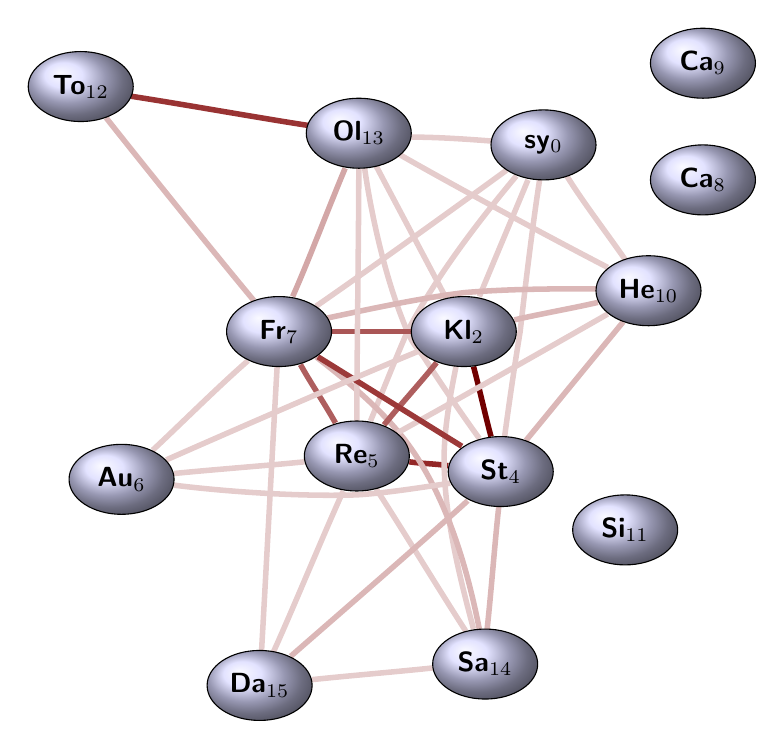
\begin{tikzpicture}[>=latex,join=bevel,scale=0.7]
%  \pgfsetlinewidth{1bp}
%%
\pgfsetcolor{black}
  % Edge: u5 -- u0
  \draw [color=black!50!red!20.0,line width=2] (177bp,155bp) .. controls (182bp,167bp) and (189bp,185bp)  .. (196bp,201bp) .. controls (212bp,232bp) and (237bp,263bp)  .. (252bp,281bp);
  % Edge: u15 -- u7
  \draw [color=black!50!red!20.0,line width=2] (121bp,37bp) .. controls (123bp,72bp) and (127bp,148bp)  .. (129bp,183bp);
  % Edge: u13 -- u4
  \draw [color=black!50!red!20.0,line width=2] (174bp,285bp) .. controls (177bp,264bp) and (184bp,229bp)  .. (196bp,201bp) .. controls (199bp,194bp) and (201bp,193bp)  .. (205bp,187bp) .. controls (214bp,173bp) and (225bp,157bp)  .. (233bp,146bp);
  % Edge: u7 -- u2
  \draw [color=black!50!red!66.332495807108,line width=2] (157bp,201bp) .. controls (170bp,201bp) and (185bp,201bp)  .. (198bp,201bp);
  % Edge: u5 -- u4
  \draw [color=black!50!red!84.8528137423857,line width=2] (197bp,134bp) .. controls (204bp,133bp) and (211bp,133bp)  .. (217bp,132bp);
  % Edge: u7 -- u6
  \draw [color=black!50!red!20.0,line width=2] (114bp,186bp) .. controls (99bp,173bp) and (79bp,153bp)  .. (65bp,140bp);
  % Edge: u13 -- u0
  \draw [color=black!50!red!20.0,line width=2] (198bp,301bp) .. controls (211bp,301bp) and (226bp,300bp)  .. (239bp,299bp);
  % Edge: u14 -- u2
  \draw [color=black!50!red!20.0,line width=2] (230bp,48bp) .. controls (225bp,67bp) and (216bp,100bp)  .. (215bp,129bp) .. controls (214bp,147bp) and (218bp,168bp)  .. (221bp,183bp);
  % Edge: u4 -- u10
  \draw [color=black!50!red!28.2842712474619,line width=2] (257bp,145bp) .. controls (271bp,162bp) and (293bp,189bp)  .. (307bp,206bp);
  % Edge: u7 -- u5
  \draw [color=black!50!red!63.2455532033676,line width=2] (141bp,184bp) .. controls (146bp,175bp) and (154bp,163bp)  .. (159bp,154bp);
  % Edge: u13 -- u12
  \draw [color=black!50!red!80.0,line width=2] (145bp,307bp) .. controls (119bp,311bp) and (80bp,318bp)  .. (54bp,322bp);
  % Edge: u4 -- u2
  \draw [color=black!50!red!111.3552872566,line width=2] (239bp,147bp) .. controls (236bp,158bp) and (233bp,172bp)  .. (230bp,183bp);
  % Edge: u14 -- u7
  \draw [color=black!50!red!28.2842712474619,line width=2] (233bp,48bp) .. controls (228bp,73bp) and (217bp,120bp)  .. (190bp,151bp) .. controls (178bp,165bp) and (162bp,178bp)  .. (149bp,188bp);
  % Edge: u10 -- u0
  \draw [color=black!50!red!20.0,line width=2] (308bp,238bp) .. controls (299bp,251bp) and (286bp,268bp)  .. (278bp,281bp);
  % Edge: u13 -- u7
  \draw [color=black!50!red!34.6410161513775,line width=2] (164bp,285bp) .. controls (156bp,266bp) and (145bp,237bp)  .. (137bp,219bp);
  % Edge: u5 -- u2
  \draw [color=black!50!red!63.2455532033676,line width=2] (184bp,153bp) .. controls (192bp,163bp) and (203bp,175bp)  .. (211bp,185bp);
  % Edge: u5 -- u10
  \draw [color=black!50!red!20.0,line width=2] (191bp,149bp) .. controls (220bp,165bp) and (271bp,194bp)  .. (299bp,210bp);
  % Edge: u2 -- u0
  \draw [color=black!50!red!20.0,line width=2] (233bp,219bp) .. controls (240bp,236bp) and (251bp,262bp)  .. (258bp,279bp);
  % Edge: u15 -- u14
  \draw [color=black!50!red!20.0,line width=2] (147bp,22bp) .. controls (166bp,24bp) and (190bp,26bp)  .. (209bp,28bp);
  % Edge: u14 -- u4
  \draw [color=black!50!red!28.2842712474619,line width=2] (237bp,48bp) .. controls (239bp,66bp) and (241bp,93bp)  .. (243bp,111bp);
  % Edge: u7 -- u0
  \draw [color=black!50!red!20.0,line width=2] (149bp,214bp) .. controls (175bp,232bp) and (221bp,265bp)  .. (247bp,284bp);
  % Edge: u6 -- u4
  \draw [color=black!50!red!20.0,line width=2] (76bp,122bp) .. controls (100bp,119bp) and (138bp,116bp)  .. (170bp,117bp) .. controls (186bp,118bp) and (204bp,121bp)  .. (218bp,123bp);
  % Edge: u15 -- u5
  \draw [color=black!50!red!20.0,line width=2] (127bp,36bp) .. controls (137bp,58bp) and (153bp,97bp)  .. (163bp,119bp);
  % Edge: u13 -- u10
  \draw [color=black!50!red!20.0,line width=2] (192bp,292bp) .. controls (220bp,276bp) and (270bp,249bp)  .. (299bp,234bp);
  % Edge: u13 -- u2
  \draw [color=black!50!red!20.0,line width=2] (180bp,286bp) .. controls (190bp,267bp) and (206bp,237bp)  .. (216bp,218bp);
  % Edge: u4 -- u0
  \draw [color=black!50!red!20.0,line width=2] (246bp,147bp) .. controls (248bp,162bp) and (251bp,183bp)  .. (254bp,201bp) .. controls (257bp,228bp) and (261bp,260bp)  .. (264bp,279bp);
  % Edge: u14 -- u5
  \draw [color=black!50!red!20.0,line width=2] (226bp,47bp) .. controls (213bp,67bp) and (193bp,100bp)  .. (180bp,120bp);
  % Edge: u6 -- u5
  \draw [color=black!50!red!20.0,line width=2] (76bp,128bp) .. controls (96bp,130bp) and (123bp,132bp)  .. (143bp,134bp);
  % Edge: u15 -- u4
  \draw [color=black!50!red!28.2842712474619,line width=2] (136bp,34bp) .. controls (160bp,55bp) and (204bp,93bp)  .. (227bp,114bp);
  % Edge: u7 -- u10
  \draw [color=black!50!red!28.2842712474619,line width=2] (155bp,208bp) .. controls (174bp,212bp) and (201bp,218bp)  .. (225bp,221bp) .. controls (248bp,223bp) and (274bp,223bp)  .. (293bp,223bp);
  % Edge: u13 -- u5
  \draw [color=black!50!red!20.0,line width=2] (171bp,285bp) .. controls (171bp,253bp) and (170bp,187bp)  .. (170bp,155bp);
  % Edge: u12 -- u7
  \draw [color=black!50!red!28.2842712474619,line width=2] (41bp,311bp) .. controls (60bp,287bp) and (97bp,241bp)  .. (117bp,217bp);
  % Edge: u7 -- u4
  \draw [color=black!50!red!77.4596669241483,line width=2] (150bp,188bp) .. controls (171bp,175bp) and (203bp,155bp)  .. (224bp,142bp);
  % Edge: u10 -- u2
  \draw [color=black!50!red!28.2842712474619,line width=2] (294bp,216bp) .. controls (281bp,213bp) and (264bp,210bp)  .. (251bp,207bp);
  % Edge: u6 -- u2
  \draw [color=black!50!red!20.0,line width=2] (72bp,135bp) .. controls (106bp,150bp) and (168bp,177bp)  .. (202bp,191bp);
  % Node: u9
\begin{scope}
  \pgfsetstrokecolor{black}
  \draw [ball color=blue!15] (348bp,339bp) ellipse (27bp and 18bp);
  \draw (348bp,339bp) node {\textbf{\textsf{Ca}}$_{9}$};
\end{scope}
  % Node: u8
\begin{scope}
  \pgfsetstrokecolor{black}
  \draw [ball color=blue!15] (348bp,279bp) ellipse (27bp and 18bp);
  \draw (348bp,279bp) node {\textbf{\textsf{Ca}}$_{8}$};
\end{scope}
  % Node: u5
\begin{scope}
  \pgfsetstrokecolor{black}
  \draw [ball color=blue!15] (170bp,137bp) ellipse (27bp and 18bp);
  \draw (170bp,137bp) node {\textbf{\textsf{Re}}$_{5}$};
\end{scope}
  % Node: u4
\begin{scope}
  \pgfsetstrokecolor{black}
  \draw [ball color=blue!15] (244bp,129bp) ellipse (27bp and 18bp);
  \draw (244bp,129bp) node {\textbf{\textsf{St}}$_{4}$};
\end{scope}
  % Node: u7
\begin{scope}
  \pgfsetstrokecolor{black}
  \draw [ball color=blue!15] (130bp,201bp) ellipse (27bp and 18bp);
  \draw (130bp,201bp) node {\textbf{\textsf{Fr}}$_{7}$};
\end{scope}
  % Node: u6
\begin{scope}
  \pgfsetstrokecolor{black}
  \draw [ball color=blue!15] (49bp,125bp) ellipse (27bp and 18bp);
  \draw (49bp,125bp) node {\textbf{\textsf{Au}}$_{6}$};
\end{scope}
  % Node: u0
\begin{scope}
  \pgfsetstrokecolor{black}
  \draw [ball color=blue!15] (266bp,297bp) ellipse (27bp and 18bp);
  \draw (266bp,297bp) node {\textbf{\textsf{sy}}$_{0}$};
\end{scope}
  % Node: u2
\begin{scope}
  \pgfsetstrokecolor{black}
  \draw [ball color=blue!15] (225bp,201bp) ellipse (27bp and 18bp);
  \draw (225bp,201bp) node {\textbf{\textsf{Kl}}$_{2}$};
\end{scope}
  % Node: u11
\begin{scope}
  \pgfsetstrokecolor{black}
  \draw [ball color=blue!15] (308bp,99bp) ellipse (27bp and 18bp);
  \draw (308bp,99bp) node {\textbf{\textsf{Si}}$_{11}$};
\end{scope}
  % Node: u10
\begin{scope}
  \pgfsetstrokecolor{black}
  \draw [ball color=blue!15] (320bp,222bp) ellipse (27bp and 18bp);
  \draw (320bp,222bp) node {\textbf{\textsf{He}}$_{10}$};
\end{scope}
  % Node: u13
\begin{scope}
  \pgfsetstrokecolor{black}
  \draw [ball color=blue!15] (171bp,303bp) ellipse (27bp and 18bp);
  \draw (171bp,303bp) node {\textbf{\textsf{Ol}}$_{13}$};
\end{scope}
  % Node: u12
\begin{scope}
  \pgfsetstrokecolor{black}
  \draw [ball color=blue!15] (28bp,327bp) ellipse (27bp and 18bp);
  \draw (28bp,327bp) node {\textbf{\textsf{To}}$_{12}$};
\end{scope}
  % Node: u15
\begin{scope}
  \pgfsetstrokecolor{black}
  \draw [ball color=blue!15] (120bp,19bp) ellipse (27bp and 18bp);
  \draw (120bp,19bp) node {\textbf{\textsf{Da}}$_{15}$};
\end{scope}
  % Node: u14
\begin{scope}
  \pgfsetstrokecolor{black}
  \draw [ball color=blue!15] (236bp,30bp) ellipse (27bp and 18bp);
  \draw (236bp,30bp) node {\textbf{\textsf{Sa}}$_{14}$};
\end{scope}
%
\end{tikzpicture}


%%% Local Variables: 
%%% mode: latex
%%% TeX-master: "tutorial"
%%% End: 

  \caption{Graphviz, \LaTeX\ and Tikz working together}
  \label{fig:tikz_ca}
\end{figure}

Graphviz output is really nice. And there is even a way to improve the
quality of the rendering if you use \LaTeX\ (and Tikz) to produce your high
quality documents (well, I use it for nearly every document, including
this tutorial), and if you have
\code{dot2tex}\footnote{\url{http://www.fauskes.net/code/dot2tex/}}
installed. If you want to stay away from the world of good and fast typography and have no connection to \LaTeX\ you may simply skip this section.

\rdoc{Dotgraph.to\_texfile} uses \code{graphviz} and \code{dot2tex} to
create a \LaTeX-file (figure~\ref{fig:tikz_ca}):%
\begin{typed}
\p{irb(main):206:0>} \c{cgraph.nodeblock \{ |u| 
\hfill "\textbackslash\textbackslash\textbackslash\textbackslash{}textbf\{#\{u.name[0..1]\}\}$_\{#\{u.uid\}\}$" \}}
=> #<Proc:0xf66f7100@(irb):206>
\p{irb(main):207:0>} \c{cgraph.to_texfile('gv_ca.tex',:alg => :neato, :fmt => 'tikz', 
                     :attrs => ['overlap=false', 'splines=true', 
                'node [fixedsize, style="ball color=blue!15, semitransparent"]',
                'edge [len=2]']) \{ |w| 
\hfill ["style=\textbackslash"color=black!50!red!#\{w**0.5*20\}, line width=2\textbackslash""] \}}
=> #<File:~/mwparser/gv_ca.tex (closed)>
\end{typed}
Using tikz has two main advantages: node and edge labels may contain
arbitrary \LaTeX-code (used here for bold fonts and subscripted uids)
and all graphical elements can use the full power of Tikz for
rendering\footnote{have a look in the \code{dot2tex}
  (\url{http://www.fauskes.net/code/dot2tex/gallery/}) and the Tikz/PGF
  (\url{http://www.texample.net/tikz/examples/}) galleries for
  impressing examples.} (see our shiny nodes).

\subsection{Graph Animations}
\label{sec:sonia}

I promised you in section~\ref{sec:graphmethods} to tell you more
about how to create nice animantions. The method 
\rdoc{Mediawiki::Wiki.timedinterlockingresponsegraph} gives an
interlocking response graph of our wiki where each response is denoted
by an explicit link attributed by the time stamp of the
response. Dotgraph is able to create
SoNIA\footnote{\url{www.stanford.edu/group/sonia/}} animation source
files if the graph contains edges attributed with timestamps.
So all we have to do is:
\begin{typed}
\p{irb(main):063:0>} \c{wiki.timedinterlockingresponsegraph.to_sonfile('il.son') }
=> #<File:~/mwparser/il.son (closed)>
\end{typed}
\cmd{to\_sonfile} takes various parameters which allow to finetune node
and edge appearance in the animation. The defaults should give you a
good starting point.

Now we can start SoNIA, load \file{il.son} and create nice animations
like the ones you can see at
\url{http://www.kinf.wiai.uni-bamberg.de/mwstat/Inhalt.html}.
How to use SoNIA is beyond this tutorial, sorry.

Creating son-files certainly works on any graph if you provide timed links.


\section{Writing Scripts}
\label{sec:scripts}

Up to now we used WikiExplorator interactively with \code{irb}. Ruby
is a full-featured programming language, so we may want to write some
ruby programs for our work. So I use my favourite editor to open
\file{myscript.rb}:
\begin{File}
\rem{#!/usr/bin/ruby -w}
require 'mediawiki/full'  \rem{# load all parts of the WikiExplorator library}
\rem{# now we open our wiki:}
wiki = Mediawiki::Wiki.open("wiodb", "wiowiki.kinf.wiai.uni-bamberg.de",
                            "wiouser", IO.getpw,
                            :language => 'de', :name => 'WiO')
wiki.pp_global_userstats  \rem{# and some output. More should follow}
\end{File}
The first line tells unixoide platforms that this is a ruby
script. Then we require the \file{mediawiki/full} library and now we
can open our wiki. I did not save the password in the script but ask
the user to type it in using \cmd{IO.getpw}. And finally I print ouzt
some statistics.

Alternatively we could have used the startup file we created before:
\begin{File}
\rem{#!/usr/bin/ruby -w}
require 'wio'                            \rem{# load the startup file}
wiki = Mediawiki.mywiki(IO.getpw)        \rem{# open the wiki}
wiki.pp_global_userstats                 \rem{# some output}
puts "My personnel wiki statistic tool!" \rem{# Hurray!}
\end{File}

So, go and learn some Ruby, write nice methods for sophisticated
statistics and visualization and send them to me to be integrated in
the codebase.

\section{Customized Reports}
\label{sec:reports}

Besides interactive usage and specially written programs
WikiExplorator is also able to do nice wiki reports as PDF or
HTML:\footnote{The same command line is also used in our startup
  file.}
\begin{typed}
\p{irb(main):117:0>} \c{Mediawiki::Report.new(wiki, :pdf, :template => 'web', 
                                       :outputdir => 'mw-report').generate}
Reading './mediawiki/reports/web.de.tex' failed. 
Trying './mediawiki/reports/web.tex'.
Found some NaN's! Removed!
This is pdfTeXk, Version 3.141592-1.40.3 (Web2C 7.5.6)
 %&-line parsing enabled.
entering extended mode
=> "~/mwparser/mw-report/default.pdf"
\end{typed}
This generates a report with template ``\code{web}'' in the output
directory ``\file{mw-report}''. As you can see in the next line
WikiExplorator first tries to find a report file with the right
language (``\cmd{de}'' for our example wiki) and falls back to the
default file. And finally the path of the report is returned.

We may want to create an own report customized to our needs. Let's
create our own HTML report by creating a new file
``\file{mediawiki/reports/myreport.html}''
(figure~\ref{fig:myreport.html}). It is an ordinary HTML file with
ruby commands embedded (this is similar to PHP). Embedded commands are
enclosed in \cmd{<\%\dots\%>} or \cmd{<\%=\dots\%>}. The latter form
includes the return value of the command in the resulting HTML file.

As you can see we use \cmd{@wiki} to access our wiki. The ``\cmd{@}''
indicates ruby instance variables and within the report file
WikiExplorator provides the wiki to us in the instance variable
\cmd{@wiki}. 


\begin{figure}
  \centering
  \begin{File}
<!DOCTYPE HTML PUBLIC "-//W3C//DTD HTML 4.01 Transitional//EN">
<html>
  <head>
    <title>My report: \cmd{<%= @wiki.to_s %>}</title>
  </head>
  \cmd{<% full = @wiki.filter.clone; full.include_all_namespaces %>}
  \cmd{<% wiki.filter.namespace=0 %>}
  \cmd{<% users = @wiki.users %>}
  \cmd{<% pages = @wiki.pages %>}
  \cmd{<% revisions = @wiki.revisions %>}
  <body>
    <h1>My report: \cmd{<%= @wiki.name %>}</h1>
    <p>
      We have \cmd{<%=@wiki.pages(full).length%>} pages with 
      \cmd{<%=@wiki.revisions(full).length%>} revisions from 
      \cmd{<%=users.length%>} users (\cmd{<%=pages.length%>} pages with
      \cmd{<%=revisions.length%>} revisions in Namespace 0).
    </p>
    \cmd{<% up = users.collect \{ |u| u.pages.length \}
       up.gp_plot_lorenz(:title => "Lorenz Curve", :xlabel => "authors", 
                         :ylabel => "pages", :png=>'cdfap.png', 
                         :size => '480,480')
    %>}
    <p>
      <img alt="lorenz curve - pages vs. authors" src="cdfap.png" />
    </p>
  </body>
</html>
\end{File}
  \caption{\file{mediawiki/reports/myreport.html}}
  \label{fig:myreport.html}\vspace{4ex}

\setlength{\fboxsep}{2ex}
\fbox{\parbox{.9\textwidth}{
\textbf{\sffamily\Large My report: WiO}\\[2ex]
We have 271 pages with 1362 revisions from 14 users (109 pages with 1125 revisions in Namespace 0).\\
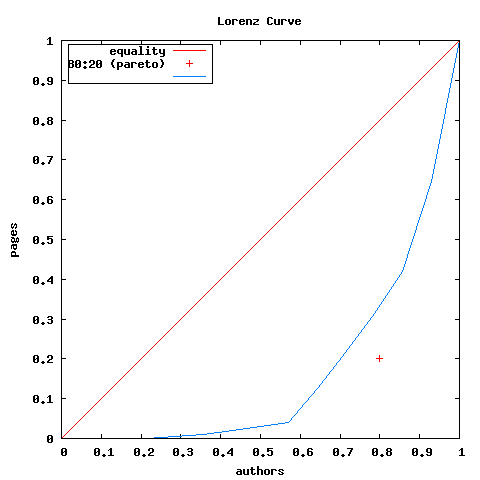
\includegraphics[width=.3\linewidth]{cdfap.png}
}}
  \caption{output for \file{myreport.html}}
  \label{fig:myreport.html-output}
\end{figure}

So what we are doing here is to create a second filter
(``\cmd{full}'') including all namespaces, set some local variables
and write some text with embedded commands giving simple descriptive
statistics about the wiki. Then we create some nice graphic and
point to it using the ``\code{img}'' tag.

Try it:
\begin{typed}
\p{irb(main):126:0>} \c{Mediawiki::Report.new(wiki, :html, :template => 'myreport', 
                                       :outputdir => '/tmp/mw-report').generate}
Reading './mediawiki/reports/myreport.de.html' failed. 
Trying './mediawiki/reports/myreport.html'.
=> "~/mwparser/mw-report/default.html"
\end{typed}
As you can see first the language specific file was tried and as it
was missing WikiExplorator fell back to the default.  

Now point your webbrowser to
``\file{\~{}/mwparser/mw-report/default.html}'' and see the result
(figure~\ref{fig:myreport.html-output}).

Creating \LaTeX/PDF templates works the same way. Use the files in
``\file{mediawiki/reports/}'' as starting point for own reports, but
save them under new names (otherwise you would loose then on update).

And do not forget to send them to me for inclusion in the
WikiExplorator package, I am interested in new interesting reports, in
translations of reports to other languages etc., in all kinds of
improvements.

\section{Acknowledgements}
\label{sec:ack}

Wiki Explorator\footnote{\url{http://wiki-explorator.rubyforge.org}} 
was developed\footnote{in the WiO project supported by a grant from the
  Volkswagen Stiftung.} by\\[2ex]
Dr.\,Klaus Stein\\
Laboratory for Semantic Information Technology\\
Chair of Computing in the Cultural Sciences\\
Otto-Friedrich Univerity Bamberg\\[2ex]
and is available as open source.


\bibliographystyle{alpha}
\bibliography{tutorial}

\end{document}
